\documentclass[twoside]{book}

% Packages required by doxygen
\usepackage{fixltx2e}
\usepackage{calc}
\usepackage{doxygen}
\usepackage[export]{adjustbox} % also loads graphicx
\usepackage{graphicx}
\usepackage[utf8]{inputenc}
\usepackage{makeidx}
\usepackage{multicol}
\usepackage{multirow}
\PassOptionsToPackage{warn}{textcomp}
\usepackage{textcomp}
\usepackage[nointegrals]{wasysym}
\usepackage[table]{xcolor}

% Font selection
\usepackage[T1]{fontenc}
\usepackage[scaled=.90]{helvet}
\usepackage{courier}
\usepackage{amssymb}
\usepackage{sectsty}
\renewcommand{\familydefault}{\sfdefault}
\allsectionsfont{%
  \fontseries{bc}\selectfont%
  \color{darkgray}%
}
\renewcommand{\DoxyLabelFont}{%
  \fontseries{bc}\selectfont%
  \color{darkgray}%
}
\newcommand{\+}{\discretionary{\mbox{\scriptsize$\hookleftarrow$}}{}{}}

% Page & text layout
\usepackage{geometry}
\geometry{%
  a4paper,%
  top=2.5cm,%
  bottom=2.5cm,%
  left=2.5cm,%
  right=2.5cm%
}
\tolerance=750
\hfuzz=15pt
\hbadness=750
\setlength{\emergencystretch}{15pt}
\setlength{\parindent}{0cm}
\setlength{\parskip}{3ex plus 2ex minus 2ex}
\makeatletter
\renewcommand{\paragraph}{%
  \@startsection{paragraph}{4}{0ex}{-1.0ex}{1.0ex}{%
    \normalfont\normalsize\bfseries\SS@parafont%
  }%
}
\renewcommand{\subparagraph}{%
  \@startsection{subparagraph}{5}{0ex}{-1.0ex}{1.0ex}{%
    \normalfont\normalsize\bfseries\SS@subparafont%
  }%
}
\makeatother

% Headers & footers
\usepackage{fancyhdr}
\pagestyle{fancyplain}
\fancyhead[LE]{\fancyplain{}{\bfseries\thepage}}
\fancyhead[CE]{\fancyplain{}{}}
\fancyhead[RE]{\fancyplain{}{\bfseries\leftmark}}
\fancyhead[LO]{\fancyplain{}{\bfseries\rightmark}}
\fancyhead[CO]{\fancyplain{}{}}
\fancyhead[RO]{\fancyplain{}{\bfseries\thepage}}
\fancyfoot[LE]{\fancyplain{}{}}
\fancyfoot[CE]{\fancyplain{}{}}
\fancyfoot[RE]{\fancyplain{}{\bfseries\scriptsize Generated by Doxygen }}
\fancyfoot[LO]{\fancyplain{}{\bfseries\scriptsize Generated by Doxygen }}
\fancyfoot[CO]{\fancyplain{}{}}
\fancyfoot[RO]{\fancyplain{}{}}
\renewcommand{\footrulewidth}{0.4pt}
\renewcommand{\chaptermark}[1]{%
  \markboth{#1}{}%
}
\renewcommand{\sectionmark}[1]{%
  \markright{\thesection\ #1}%
}

% Indices & bibliography
\usepackage{natbib}
\usepackage[titles]{tocloft}
\setcounter{tocdepth}{3}
\setcounter{secnumdepth}{5}
\makeindex

% Hyperlinks (required, but should be loaded last)
\usepackage{ifpdf}
\ifpdf
  \usepackage[pdftex,pagebackref=true]{hyperref}
\else
  \usepackage[ps2pdf,pagebackref=true]{hyperref}
\fi
\hypersetup{%
  colorlinks=true,%
  linkcolor=blue,%
  citecolor=blue,%
  unicode%
}

% Custom commands
\newcommand{\clearemptydoublepage}{%
  \newpage{\pagestyle{empty}\cleardoublepage}%
}

\usepackage{caption}
\captionsetup{labelsep=space,justification=centering,font={bf},singlelinecheck=off,skip=4pt,position=top}

%===== C O N T E N T S =====

\begin{document}

% Titlepage & ToC
\hypersetup{pageanchor=false,
             bookmarksnumbered=true,
             pdfencoding=unicode
            }
\pagenumbering{alph}
\begin{titlepage}
\vspace*{7cm}
\begin{center}%
{\Large C++ Web Framework \\[1ex]\large 3.\+0 }\\
\vspace*{1cm}
{\large Generated by Doxygen 1.8.13}\\
\end{center}
\end{titlepage}
\clearemptydoublepage
\pagenumbering{roman}
\tableofcontents
\clearemptydoublepage
\pagenumbering{arabic}
\hypersetup{pageanchor=true}

%--- Begin generated contents ---
\chapter{The C++ Web Framework}
\label{index}\hypertarget{index}{}The C++ Web Framework (C\+WF) is an Open Source web framework, under M\+IT License, created by Herik Lima and Marcelo Eler, using C++ with Qt to be used in the development of web applications, having been heavily inspired by Java Servlets, Java\+Server Pages Standard Tag Library (J\+S\+TL), designed to consume few computational resources such as memory and processing and a low response time for requests. The C\+WF also adopts the M\+VC (Model-\/\+View-\/\+Controller) architecture, where you can create classes to take care of the business layer (Model), use C\+S\+TL (C++ Server Pages Standard Tag Library) within the Web Pages to take care of data presentation (View) and use the servlets as a between the two layers (Controller).

Because it is created in Qt, the C++ Web Framework can run on the same platforms supported by Qt\+: ~\newline


Desktop\+: Linux, OS X, Windows~\newline
 Embedded and R\+T\+OS\+: Linux, Q\+NX, Vx\+Works, Windows~\newline
 Mobile\+: Android, i\+OS, Windows~\newline


This web framework consists of a simplified set of classes, only one configuration file, called C\+P\+P\+Web.\+ini and a policy of using only C++ and Qt in the development of its components in order to avoid the installation of numerous libraries to avoid conflicts, maintain multiplatform characteristics, facilitate installation and keep the learning curve low in order to make web development as simple as possible, even for beginners. 
\chapter{Hierarchical Index}
\section{Class Hierarchy}
This inheritance list is sorted roughly, but not completely, alphabetically\+:\begin{DoxyCompactList}
\item \contentsline{section}{Configuration}{\pageref{class_configuration}}{}
\item \contentsline{section}{Controller}{\pageref{class_controller}}{}
\begin{DoxyCompactList}
\item \contentsline{section}{Cpp\+Web\+Controller}{\pageref{class_cpp_web_controller}}{}
\end{DoxyCompactList}
\item \contentsline{section}{Cpp\+Web\+Application}{\pageref{class_cpp_web_application}}{}
\item \contentsline{section}{C\+S\+T\+L\+Compiler}{\pageref{class_c_s_t_l_compiler}}{}
\item \contentsline{section}{C\+S\+T\+L\+Compiler\+Attributes}{\pageref{class_c_s_t_l_compiler_attributes}}{}
\item \contentsline{section}{C\+S\+T\+L\+Compiler\+For}{\pageref{class_c_s_t_l_compiler_for}}{}
\item \contentsline{section}{C\+S\+T\+L\+Compiler\+If}{\pageref{class_c_s_t_l_compiler_if}}{}
\item \contentsline{section}{C\+S\+T\+L\+Compiler\+Import}{\pageref{class_c_s_t_l_compiler_import}}{}
\item \contentsline{section}{File\+Manager}{\pageref{class_file_manager}}{}
\item \contentsline{section}{Filter}{\pageref{class_filter}}{}
\item \contentsline{section}{Filter\+Chain}{\pageref{class_filter_chain}}{}
\item \contentsline{section}{Http\+Parser}{\pageref{class_http_parser}}{}
\item \contentsline{section}{Meta\+Class\+Parser}{\pageref{class_meta_class_parser}}{}
\item \contentsline{section}{Properties}{\pageref{class_properties}}{}
\item \contentsline{section}{Q\+Map\+Thread\+Safety$<$ Key, T $>$}{\pageref{class_q_map_thread_safety}}{}
\item \contentsline{section}{Q\+Map\+Thread\+Safety$<$ Q\+String, Controller $\ast$$>$}{\pageref{class_q_map_thread_safety}}{}
\item \contentsline{section}{Q\+Map\+Thread\+Safety$<$ Q\+String, Q\+Object $\ast$$>$}{\pageref{class_q_map_thread_safety}}{}
\item \contentsline{section}{Q\+Map\+Thread\+Safety$<$ Q\+String, Session $\ast$$>$}{\pageref{class_q_map_thread_safety}}{}
\item Q\+Object\begin{DoxyCompactList}
\item \contentsline{section}{C\+S\+T\+L\+Compiler\+Object}{\pageref{class_c_s_t_l_compiler_object}}{}
\item \contentsline{section}{Q\+List\+Object}{\pageref{class_q_list_object}}{}
\item \contentsline{section}{Variant}{\pageref{class_variant}}{}
\end{DoxyCompactList}
\item Q\+Runnable\begin{DoxyCompactList}
\item \contentsline{section}{Http\+Read\+Request}{\pageref{class_http_read_request}}{}
\end{DoxyCompactList}
\item Q\+Sql\+Query\begin{DoxyCompactList}
\item \contentsline{section}{Sql\+Query}{\pageref{class_sql_query}}{}
\end{DoxyCompactList}
\item Q\+Tcp\+Server\begin{DoxyCompactList}
\item \contentsline{section}{Cpp\+Web\+Server}{\pageref{class_cpp_web_server}}{}
\end{DoxyCompactList}
\item \contentsline{section}{Request}{\pageref{class_request}}{}
\item \contentsline{section}{Request\+Dispatcher}{\pageref{class_request_dispatcher}}{}
\item \contentsline{section}{Response}{\pageref{class_response}}{}
\item \contentsline{section}{Session}{\pageref{class_session}}{}
\item \contentsline{section}{Sql\+Database\+Storage}{\pageref{class_sql_database_storage}}{}
\item \contentsline{section}{Ssl\+Loader}{\pageref{class_ssl_loader}}{}
\item \contentsline{section}{U\+R\+L\+Encoder}{\pageref{class_u_r_l_encoder}}{}
\end{DoxyCompactList}

\chapter{Class Index}
\section{Class List}
Here are the classes, structs, unions and interfaces with brief descriptions\+:\begin{DoxyCompactList}
\item\contentsline{section}{\mbox{\hyperlink{class_configuration}{Configuration}} \\*All classes of C++ Web Framework are contained within the namespace C\+WF }{\pageref{class_configuration}}{}
\item\contentsline{section}{\mbox{\hyperlink{class_cpp_web_application}{Cpp\+Web\+Application}} \\*This class is responsible for encapsulating the Q\+Core\+Application, the \mbox{\hyperlink{class_cpp_web_server}{Cpp\+Web\+Server}} and configure the server logging mechanism }{\pageref{class_cpp_web_application}}{}
\item\contentsline{section}{\mbox{\hyperlink{class_cpp_web_server}{Cpp\+Web\+Server}} \\*H\+T\+TP server, responsable to receive and dispatch the requisitions }{\pageref{class_cpp_web_server}}{}
\item\contentsline{section}{\mbox{\hyperlink{class_cpp_web_servlet}{Cpp\+Web\+Servlet}} \\*This class is responsible for displaying the standard pages of C++ Web Framework\+: index, examples, documentation, ssl and authors }{\pageref{class_cpp_web_servlet}}{}
\item\contentsline{section}{\mbox{\hyperlink{class_c_s_t_l_compiler}{C\+S\+T\+L\+Compiler}} \\*This class compiles xhtml pages with C\+S\+TL (C++ Server Pages Standard Tags Library) }{\pageref{class_c_s_t_l_compiler}}{}
\item\contentsline{section}{\mbox{\hyperlink{class_c_s_t_l_compiler_attributes}{C\+S\+T\+L\+Compiler\+Attributes}} \\*This class search for expressions \#\{obj.\+get\} and compiles it }{\pageref{class_c_s_t_l_compiler_attributes}}{}
\item\contentsline{section}{\mbox{\hyperlink{class_c_s_t_l_compiler_for}{C\+S\+T\+L\+Compiler\+For}} \\*Extracts and valites all attibutes from a \char`\"{}for\char`\"{} tag }{\pageref{class_c_s_t_l_compiler_for}}{}
\item\contentsline{section}{\mbox{\hyperlink{class_c_s_t_l_compiler_if}{C\+S\+T\+L\+Compiler\+If}} \\*Extracts and valites all attibutes from a \char`\"{}if\char`\"{} tag }{\pageref{class_c_s_t_l_compiler_if}}{}
\item\contentsline{section}{\mbox{\hyperlink{class_c_s_t_l_compiler_import}{C\+S\+T\+L\+Compiler\+Import}} \\*Extracts and valites all attibutes from a \char`\"{}import\char`\"{} tag }{\pageref{class_c_s_t_l_compiler_import}}{}
\item\contentsline{section}{\mbox{\hyperlink{class_c_s_t_l_compiler_object}{C\+S\+T\+L\+Compiler\+Object}} \\*The \mbox{\hyperlink{class_properties}{Properties}} class is an auxiliar class to the \mbox{\hyperlink{class_c_s_t_l_compiler}{C\+S\+T\+L\+Compiler}} }{\pageref{class_c_s_t_l_compiler_object}}{}
\item\contentsline{section}{\mbox{\hyperlink{class_file_manager}{File\+Manager}} \\*Can manage file\textquotesingle{}s name }{\pageref{class_file_manager}}{}
\item\contentsline{section}{\mbox{\hyperlink{class_filter}{Filter}} \\*Works like a filter. You can use this class to validate sessions or measuring runtime of a specific method, for example. To use this class, you will need to create a derived class and reconstruct the do\+Filter method, after this, you will need to configure it into the Configure\+Cpp\+Web\+Server, using the set\+Filter method }{\pageref{class_filter}}{}
\item\contentsline{section}{\mbox{\hyperlink{class_filter_chain}{Filter\+Chain}} \\*Responsable to dispatch a requisition. This class was built to work with \mbox{\hyperlink{class_filter}{Filter}}. Always when a \mbox{\hyperlink{class_filter}{Filter}} makes all the necessary validations, it can dispatches the requisition to the \mbox{\hyperlink{class_filter_chain}{Filter\+Chain}}. N\+O\+TE\+: It is a final class, you can\textquotesingle{}t derive from it }{\pageref{class_filter_chain}}{}
\item\contentsline{section}{\mbox{\hyperlink{class_http_cookie}{Http\+Cookie}} \\*This class represents a H\+T\+TP Cookie }{\pageref{class_http_cookie}}{}
\item\contentsline{section}{\mbox{\hyperlink{class_http_parser}{Http\+Parser}} \\*The class parses a H\+T\+TP message }{\pageref{class_http_parser}}{}
\item\contentsline{section}{\mbox{\hyperlink{class_http_read_request}{Http\+Read\+Request}} \\*Created automatically by the \mbox{\hyperlink{class_cpp_web_server}{Cpp\+Web\+Server}} and inserted ~\newline
 in a Q\+Thread\+Pool, always when the \mbox{\hyperlink{class_cpp_web_server}{Cpp\+Web\+Server}} has a call by a client(\+Browser) }{\pageref{class_http_read_request}}{}
\item\contentsline{section}{\mbox{\hyperlink{class_http_servlet}{Http\+Servlet}} \\*Responsable to attend a request from a specific url. You will need to create a derived class from \mbox{\hyperlink{class_http_servlet}{Http\+Servlet}} and then, reconstruct the desired method to response a request, after this, you will need mapping the url to the new servlet that you created, you need to do it into the Configure\+Cpp\+Web\+Server using the method add\+Url\+Servlet }{\pageref{class_http_servlet}}{}
\item\contentsline{section}{\mbox{\hyperlink{class_http_servlet_request}{Http\+Servlet\+Request}} \\*Holds all information about a http request }{\pageref{class_http_servlet_request}}{}
\item\contentsline{section}{\mbox{\hyperlink{class_http_servlet_response}{Http\+Servlet\+Response}} \\*Responsable to response a Http request }{\pageref{class_http_servlet_response}}{}
\item\contentsline{section}{\mbox{\hyperlink{class_http_session}{Http\+Session}} \\*Holds information about a client session }{\pageref{class_http_session}}{}
\item\contentsline{section}{\mbox{\hyperlink{class_meta_class_parser}{Meta\+Class\+Parser}} \\*This class extracts all information from a Q\+Object }{\pageref{class_meta_class_parser}}{}
\item\contentsline{section}{\mbox{\hyperlink{class_properties}{Properties}} \\*Auxiliar class to the \mbox{\hyperlink{class_c_s_t_l_compiler}{C\+S\+T\+L\+Compiler}} }{\pageref{class_properties}}{}
\item\contentsline{section}{\mbox{\hyperlink{class_q_list_object}{Q\+List\+Object}} \\*Used to pass a list of object to a xhtml page. N\+O\+TE\+: Always when you need to pass a list of object to a xhtml page you will need to use this class, your class need to inherit from the Q\+Object class and all the methods needs to be in the public slots session }{\pageref{class_q_list_object}}{}
\item\contentsline{section}{\mbox{\hyperlink{class_q_map_thread_safety}{Q\+Map\+Thread\+Safety$<$ Key, T $>$}} \\*The \mbox{\hyperlink{class_q_map_thread_safety}{Q\+Map\+Thread\+Safety}} class is a thread safe Q\+Map }{\pageref{class_q_map_thread_safety}}{}
\item\contentsline{section}{\mbox{\hyperlink{class_request_dispatcher}{Request\+Dispatcher}} \\*Can be used to dispatch a requisition to a xhtml page }{\pageref{class_request_dispatcher}}{}
\item\contentsline{section}{\mbox{\hyperlink{class_sql_database_storage}{Sql\+Database\+Storage}} \\*Allows you to reuse connections made to the database through the Q\+Sql\+Database class within Q\+Thread\+Pool }{\pageref{class_sql_database_storage}}{}
\item\contentsline{section}{\mbox{\hyperlink{class_u_r_l_encoder}{U\+R\+L\+Encoder}} \\*The \mbox{\hyperlink{class_u_r_l_encoder}{U\+R\+L\+Encoder}} class }{\pageref{class_u_r_l_encoder}}{}
\item\contentsline{section}{\mbox{\hyperlink{class_variant}{Variant}} \\*This class is designed to facilitate the passing of simple type parameters such as qlonglong, double, int, and Q\+String to the C\+S\+TL (C++ Server Pages Standard Tags Library) }{\pageref{class_variant}}{}
\end{DoxyCompactList}

\chapter{Class Documentation}
\hypertarget{class_configuration}{}\section{Configuration Class Reference}
\label{class_configuration}\index{Configuration@{Configuration}}


All classes of C++ Web Framework are contained within the namespace C\+WF.  




{\ttfamily \#include $<$configuration.\+h$>$}

\subsection*{Public Member Functions}
\begin{DoxyCompactItemize}
\item 
\mbox{\hyperlink{class_configuration_af5d72b2e949b80b291b1013268cff405}{Configuration}} (Q\+String server\+Files\+Path=\char`\"{}\char`\"{})
\begin{DoxyCompactList}\small\item\em Will make reading the C\+P\+P\+Web.\+ini file and extract all of its properties. \end{DoxyCompactList}\item 
int \mbox{\hyperlink{class_configuration_a3cd126ebe20117c04b4d38797e06551d}{get\+Time\+Out}} () const
\begin{DoxyCompactList}\small\item\em Returns the time\+Out property that will be used by the server to expire threads that are not in use. Such threads will be restarted as needed. The default time\+Out is 30000 milliseconds (30 seconds). If time\+Out is negative, newly created threads will not expire, e.\+g., they will not exit until the thread pool is destroyed. \end{DoxyCompactList}\item 
void \mbox{\hyperlink{class_configuration_a4fc1c685775b37e7b553c3393f1b2998}{set\+Time\+Out}} (int value)
\begin{DoxyCompactList}\small\item\em Set the time\+Out property. \end{DoxyCompactList}\item 
int \mbox{\hyperlink{class_configuration_af14b4f22fdcdfc32fbcac712a9868fd4}{get\+Session\+Expiration\+Time}} () const
\begin{DoxyCompactList}\small\item\em Returns the time that a session takes to expire. The default is 1800000(ms). \end{DoxyCompactList}\item 
void \mbox{\hyperlink{class_configuration_a306d88e7d7c2b8394844936b49be9013}{set\+Session\+Expiration\+Time}} (int value)
\begin{DoxyCompactList}\small\item\em Set the session\+Expiration\+Time property. \end{DoxyCompactList}\item 
int \mbox{\hyperlink{class_configuration_a6a592b2194d4059f31aaf4223ee2e70e}{get\+Cleanup\+Interval}} () const
\begin{DoxyCompactList}\small\item\em Returns the cleanup\+Interval that indicates how often the server will perform the cleanup of expired sessions. \end{DoxyCompactList}\item 
void \mbox{\hyperlink{class_configuration_a5d6a822ffd2c3c029ae1864f8358a592}{set\+Cleanup\+Interval}} (int value)
\begin{DoxyCompactList}\small\item\em Set the cleanup\+Interval property that will be used by the server. The default is 86400000(ms). \end{DoxyCompactList}\item 
int \mbox{\hyperlink{class_configuration_ab34eb25aa1e175c7ac8323300b298a8a}{get\+Port}} () const
\begin{DoxyCompactList}\small\item\em Returns the port number that will be used by the server. The default is 8080. \end{DoxyCompactList}\item 
void \mbox{\hyperlink{class_configuration_aae5aafdfeb2a6e110ef8bad90a85be5e}{set\+Port}} (int value)
\begin{DoxyCompactList}\small\item\em Set the port number property. \end{DoxyCompactList}\item 
Q\+Host\+Address \mbox{\hyperlink{class_configuration_a37ca7476a8ab5a1e6c4b5a3e07670d9f}{get\+Host}} () const
\begin{DoxyCompactList}\small\item\em Returns the port number that will be used by the server. The default is 127.\+0.\+0.\+1. \end{DoxyCompactList}\item 
void \mbox{\hyperlink{class_configuration_a0851c4f93476b80acebd88204c4a86c6}{set\+Host}} (const Q\+Host\+Address \&value)
\begin{DoxyCompactList}\small\item\em Set the host property. \end{DoxyCompactList}\item 
int \mbox{\hyperlink{class_configuration_ad0e836129d0a7e0111b1f2c092729939}{get\+Max\+Thread}} () const
\begin{DoxyCompactList}\small\item\em Returns the maximum number of threads that can be created by the server. The default is 100. \end{DoxyCompactList}\item 
void \mbox{\hyperlink{class_configuration_ab242af54d85d49b88b778a50a77949a5}{set\+Max\+Thread}} (int value)
\begin{DoxyCompactList}\small\item\em Set the max\+Thread property. \end{DoxyCompactList}\item 
Q\+String \mbox{\hyperlink{class_configuration_a96082bdd3333d8ddf2017a95fe302225}{get\+Ssl\+Key\+File}} () const
\begin{DoxyCompactList}\small\item\em Retuns the ssl\+Key\+File name property that can be used by the server to make the S\+SL configuration. \end{DoxyCompactList}\item 
void \mbox{\hyperlink{class_configuration_a646d1ce1463b0519c745483a228c4949}{set\+Ssl\+Key\+File}} (const Q\+String \&value)
\begin{DoxyCompactList}\small\item\em Set the ssl\+Key\+File name property. \end{DoxyCompactList}\item 
Q\+String \mbox{\hyperlink{class_configuration_a10405dacfb3b61f60b290c0a5d79a8fb}{get\+Ssl\+Cert\+File}} () const
\begin{DoxyCompactList}\small\item\em Retuns the ssl\+Cert\+File name property that can be used by the server to make the S\+SL configuration. \end{DoxyCompactList}\item 
void \mbox{\hyperlink{class_configuration_a16eecdd98ab2b9c4737f3178656bb3ad}{set\+Ssl\+Cert\+File}} (const Q\+String \&value)
\begin{DoxyCompactList}\small\item\em Set the ssl\+Cert\+File name property. \end{DoxyCompactList}\item 
Q\+String \mbox{\hyperlink{class_configuration_a43acf80f787217903281b0a6d3e01e11}{get\+Path}} () const
\begin{DoxyCompactList}\small\item\em Returns the path should point to the server folder. \end{DoxyCompactList}\item 
void \mbox{\hyperlink{class_configuration_ade67019de7f09f22093d920fc30152e5}{set\+Path}} (const Q\+String \&value)
\begin{DoxyCompactList}\small\item\em Set the path property. \end{DoxyCompactList}\item 
Q\+String \mbox{\hyperlink{class_configuration_ab58d8dc13a90745af4925e9b238c8cff}{get\+Domain}} () const
\begin{DoxyCompactList}\small\item\em Returns the applications domain name. \end{DoxyCompactList}\item 
void \mbox{\hyperlink{class_configuration_af31a608106ec376f01acc028ccb09cb8}{set\+Domain}} (const Q\+String \&value)
\begin{DoxyCompactList}\small\item\em Set domain property. \end{DoxyCompactList}\item 
Q\+String \mbox{\hyperlink{class_configuration_a005e1d10c605e08d73ff274f2b19fc48}{get\+Log\+File\+Path}} () const
\begin{DoxyCompactList}\small\item\em Returns the path to the log file and must to be relative to the path set in the \char`\"{}path\char`\"{}. \end{DoxyCompactList}\item 
\mbox{\Hypertarget{class_configuration_a83269c31da560355e67fdf452f7e24b0}\label{class_configuration_a83269c31da560355e67fdf452f7e24b0}} 
void \mbox{\hyperlink{class_configuration_a83269c31da560355e67fdf452f7e24b0}{set\+Log\+File\+Path}} (const Q\+String \&value)
\begin{DoxyCompactList}\small\item\em Set the log\+File\+Path property. const Q\+String \&value \+: Log file path. \end{DoxyCompactList}\item 
qint64 \mbox{\hyperlink{class_configuration_a8bc88e3cfe151837ee77e213e441953e}{get\+Max\+Upload\+File}} () const
\begin{DoxyCompactList}\small\item\em Returns the maximum upload file size in bytes. \end{DoxyCompactList}\item 
void \mbox{\hyperlink{class_configuration_ada37d2f25a05d7b9fa5676f824b7e3be}{set\+Max\+Upload\+File}} (const qint64 \&value)
\begin{DoxyCompactList}\small\item\em Set max\+Upload\+File property in bytes. \end{DoxyCompactList}\item 
qint64 \mbox{\hyperlink{class_configuration_a05ee88466fbe346175ec6420b6857b98}{get\+Max\+Log\+File}} () const
\begin{DoxyCompactList}\small\item\em get\+Max\+Log\+File the max file log \end{DoxyCompactList}\item 
void \mbox{\hyperlink{class_configuration_a3c26bb11f458d7374fd4c5b53e181aee}{set\+Max\+Log\+File}} (const qint64 \&value)
\begin{DoxyCompactList}\small\item\em Set max\+Log\+File property in bytes. \end{DoxyCompactList}\end{DoxyCompactItemize}
\subsection*{Friends}
\begin{DoxyCompactItemize}
\item 
\mbox{\Hypertarget{class_configuration_af35951d3389bacc3d625fc73174f7364}\label{class_configuration_af35951d3389bacc3d625fc73174f7364}} 
class {\bfseries Cpp\+Web\+Server}
\item 
\mbox{\Hypertarget{class_configuration_a84765570a5386c96f10067fb0e11bc13}\label{class_configuration_a84765570a5386c96f10067fb0e11bc13}} 
class {\bfseries Http\+Servlet\+Response}
\item 
\mbox{\Hypertarget{class_configuration_a3e611175a551b64dda26f513067e0d04}\label{class_configuration_a3e611175a551b64dda26f513067e0d04}} 
class {\bfseries Http\+Session}
\item 
\mbox{\Hypertarget{class_configuration_a4d54f5003e07e218070a449c22a52c7c}\label{class_configuration_a4d54f5003e07e218070a449c22a52c7c}} 
class {\bfseries Http\+Read\+Request}
\item 
\mbox{\Hypertarget{class_configuration_af79af37b83b26f7eeb57dcb953a09845}\label{class_configuration_af79af37b83b26f7eeb57dcb953a09845}} 
class {\bfseries Cpp\+Web\+Application}
\item 
\mbox{\Hypertarget{class_configuration_a14d4dda0e6f3fa404ebad6cc84ab5ca6}\label{class_configuration_a14d4dda0e6f3fa404ebad6cc84ab5ca6}} 
class {\bfseries Filter\+Chain}
\end{DoxyCompactItemize}


\subsection{Detailed Description}
All classes of C++ Web Framework are contained within the namespace C\+WF. 

This class is responsable to read a ini file and extract its information. 

\subsection{Constructor \& Destructor Documentation}
\mbox{\Hypertarget{class_configuration_af5d72b2e949b80b291b1013268cff405}\label{class_configuration_af5d72b2e949b80b291b1013268cff405}} 
\index{Configuration@{Configuration}!Configuration@{Configuration}}
\index{Configuration@{Configuration}!Configuration@{Configuration}}
\subsubsection{\texorpdfstring{Configuration()}{Configuration()}}
{\footnotesize\ttfamily Configuration\+::\+Configuration (\begin{DoxyParamCaption}\item[{Q\+String}]{server\+Files\+Path = {\ttfamily \char`\"{}\char`\"{}} }\end{DoxyParamCaption})\hspace{0.3cm}{\ttfamily [explicit]}}



Will make reading the C\+P\+P\+Web.\+ini file and extract all of its properties. 


\begin{DoxyParams}{Parameters}
{\em Q\+String} & server\+Files\+Path \+: You should always points to the directory server. \\
\hline
\end{DoxyParams}
\begin{DoxyParagraph}{Example}

\begin{DoxyCode}
\textcolor{preprocessor}{#include <QCoreApplication>}
\textcolor{preprocessor}{#include <cwf/cppwebapplication.h>}

\textcolor{keywordtype}{int} main(\textcolor{keywordtype}{int} argc, \textcolor{keywordtype}{char} *argv[])
\{
    CWF::Configuration configuration(\textcolor{stringliteral}{"/home/herik/CPPWebFramework/CPPWebFramework/server/"});
    CWF::CppWebApplication a(argc, argv, configuration);

    \textcolor{keywordflow}{return} a.start();
\}
\end{DoxyCode}
 
\end{DoxyParagraph}


\subsection{Member Function Documentation}
\mbox{\Hypertarget{class_configuration_a6a592b2194d4059f31aaf4223ee2e70e}\label{class_configuration_a6a592b2194d4059f31aaf4223ee2e70e}} 
\index{Configuration@{Configuration}!get\+Cleanup\+Interval@{get\+Cleanup\+Interval}}
\index{get\+Cleanup\+Interval@{get\+Cleanup\+Interval}!Configuration@{Configuration}}
\subsubsection{\texorpdfstring{get\+Cleanup\+Interval()}{getCleanupInterval()}}
{\footnotesize\ttfamily int Configuration\+::get\+Cleanup\+Interval (\begin{DoxyParamCaption}{ }\end{DoxyParamCaption}) const}



Returns the cleanup\+Interval that indicates how often the server will perform the cleanup of expired sessions. 


\begin{DoxyParams}{Parameters}
{\em int} & \+: Time in milliseconds. \\
\hline
\end{DoxyParams}
\mbox{\Hypertarget{class_configuration_ab58d8dc13a90745af4925e9b238c8cff}\label{class_configuration_ab58d8dc13a90745af4925e9b238c8cff}} 
\index{Configuration@{Configuration}!get\+Domain@{get\+Domain}}
\index{get\+Domain@{get\+Domain}!Configuration@{Configuration}}
\subsubsection{\texorpdfstring{get\+Domain()}{getDomain()}}
{\footnotesize\ttfamily Q\+String Configuration\+::get\+Domain (\begin{DoxyParamCaption}{ }\end{DoxyParamCaption}) const}



Returns the applications domain name. 

\begin{DoxyReturn}{Returns}
Q\+String \+: Domain name. 
\end{DoxyReturn}
\mbox{\Hypertarget{class_configuration_a37ca7476a8ab5a1e6c4b5a3e07670d9f}\label{class_configuration_a37ca7476a8ab5a1e6c4b5a3e07670d9f}} 
\index{Configuration@{Configuration}!get\+Host@{get\+Host}}
\index{get\+Host@{get\+Host}!Configuration@{Configuration}}
\subsubsection{\texorpdfstring{get\+Host()}{getHost()}}
{\footnotesize\ttfamily Q\+Host\+Address Configuration\+::get\+Host (\begin{DoxyParamCaption}{ }\end{DoxyParamCaption}) const}



Returns the port number that will be used by the server. The default is 127.\+0.\+0.\+1. 

\begin{DoxyReturn}{Returns}
Q\+Host\+Address \+: Host address. 
\end{DoxyReturn}
\mbox{\Hypertarget{class_configuration_a005e1d10c605e08d73ff274f2b19fc48}\label{class_configuration_a005e1d10c605e08d73ff274f2b19fc48}} 
\index{Configuration@{Configuration}!get\+Log\+File\+Path@{get\+Log\+File\+Path}}
\index{get\+Log\+File\+Path@{get\+Log\+File\+Path}!Configuration@{Configuration}}
\subsubsection{\texorpdfstring{get\+Log\+File\+Path()}{getLogFilePath()}}
{\footnotesize\ttfamily Q\+String Configuration\+::get\+Log\+File\+Path (\begin{DoxyParamCaption}{ }\end{DoxyParamCaption}) const}



Returns the path to the log file and must to be relative to the path set in the \char`\"{}path\char`\"{}. 

\begin{DoxyReturn}{Returns}
Q\+String \+: Log File Path. 
\end{DoxyReturn}
\mbox{\Hypertarget{class_configuration_a05ee88466fbe346175ec6420b6857b98}\label{class_configuration_a05ee88466fbe346175ec6420b6857b98}} 
\index{Configuration@{Configuration}!get\+Max\+Log\+File@{get\+Max\+Log\+File}}
\index{get\+Max\+Log\+File@{get\+Max\+Log\+File}!Configuration@{Configuration}}
\subsubsection{\texorpdfstring{get\+Max\+Log\+File()}{getMaxLogFile()}}
{\footnotesize\ttfamily C\+W\+F\+\_\+\+B\+E\+G\+I\+N\+\_\+\+N\+A\+M\+E\+S\+P\+A\+CE qint64 Configuration\+::get\+Max\+Log\+File (\begin{DoxyParamCaption}{ }\end{DoxyParamCaption}) const}



get\+Max\+Log\+File the max file log 

\begin{DoxyReturn}{Returns}
qint64 \+: Max file log in bytes. 
\end{DoxyReturn}
\mbox{\Hypertarget{class_configuration_ad0e836129d0a7e0111b1f2c092729939}\label{class_configuration_ad0e836129d0a7e0111b1f2c092729939}} 
\index{Configuration@{Configuration}!get\+Max\+Thread@{get\+Max\+Thread}}
\index{get\+Max\+Thread@{get\+Max\+Thread}!Configuration@{Configuration}}
\subsubsection{\texorpdfstring{get\+Max\+Thread()}{getMaxThread()}}
{\footnotesize\ttfamily int Configuration\+::get\+Max\+Thread (\begin{DoxyParamCaption}{ }\end{DoxyParamCaption}) const}



Returns the maximum number of threads that can be created by the server. The default is 100. 

\begin{DoxyReturn}{Returns}
int \+: Maximum number of threads. 
\end{DoxyReturn}
\mbox{\Hypertarget{class_configuration_a8bc88e3cfe151837ee77e213e441953e}\label{class_configuration_a8bc88e3cfe151837ee77e213e441953e}} 
\index{Configuration@{Configuration}!get\+Max\+Upload\+File@{get\+Max\+Upload\+File}}
\index{get\+Max\+Upload\+File@{get\+Max\+Upload\+File}!Configuration@{Configuration}}
\subsubsection{\texorpdfstring{get\+Max\+Upload\+File()}{getMaxUploadFile()}}
{\footnotesize\ttfamily qint64 Configuration\+::get\+Max\+Upload\+File (\begin{DoxyParamCaption}{ }\end{DoxyParamCaption}) const}



Returns the maximum upload file size in bytes. 

\begin{DoxyReturn}{Returns}
qint64 \+: Max upload file size in bytes. 
\end{DoxyReturn}
\mbox{\Hypertarget{class_configuration_a43acf80f787217903281b0a6d3e01e11}\label{class_configuration_a43acf80f787217903281b0a6d3e01e11}} 
\index{Configuration@{Configuration}!get\+Path@{get\+Path}}
\index{get\+Path@{get\+Path}!Configuration@{Configuration}}
\subsubsection{\texorpdfstring{get\+Path()}{getPath()}}
{\footnotesize\ttfamily Q\+String Configuration\+::get\+Path (\begin{DoxyParamCaption}{ }\end{DoxyParamCaption}) const}



Returns the path should point to the server folder. 

\begin{DoxyReturn}{Returns}
Q\+String \+: Path. 
\end{DoxyReturn}
\mbox{\Hypertarget{class_configuration_ab34eb25aa1e175c7ac8323300b298a8a}\label{class_configuration_ab34eb25aa1e175c7ac8323300b298a8a}} 
\index{Configuration@{Configuration}!get\+Port@{get\+Port}}
\index{get\+Port@{get\+Port}!Configuration@{Configuration}}
\subsubsection{\texorpdfstring{get\+Port()}{getPort()}}
{\footnotesize\ttfamily int Configuration\+::get\+Port (\begin{DoxyParamCaption}{ }\end{DoxyParamCaption}) const}



Returns the port number that will be used by the server. The default is 8080. 

\begin{DoxyReturn}{Returns}
int \+: Port number. 
\end{DoxyReturn}
\mbox{\Hypertarget{class_configuration_af14b4f22fdcdfc32fbcac712a9868fd4}\label{class_configuration_af14b4f22fdcdfc32fbcac712a9868fd4}} 
\index{Configuration@{Configuration}!get\+Session\+Expiration\+Time@{get\+Session\+Expiration\+Time}}
\index{get\+Session\+Expiration\+Time@{get\+Session\+Expiration\+Time}!Configuration@{Configuration}}
\subsubsection{\texorpdfstring{get\+Session\+Expiration\+Time()}{getSessionExpirationTime()}}
{\footnotesize\ttfamily int Configuration\+::get\+Session\+Expiration\+Time (\begin{DoxyParamCaption}{ }\end{DoxyParamCaption}) const}



Returns the time that a session takes to expire. The default is 1800000(ms). 


\begin{DoxyParams}{Parameters}
{\em int} & \+: Time in milliseconds. \\
\hline
\end{DoxyParams}
\mbox{\Hypertarget{class_configuration_a10405dacfb3b61f60b290c0a5d79a8fb}\label{class_configuration_a10405dacfb3b61f60b290c0a5d79a8fb}} 
\index{Configuration@{Configuration}!get\+Ssl\+Cert\+File@{get\+Ssl\+Cert\+File}}
\index{get\+Ssl\+Cert\+File@{get\+Ssl\+Cert\+File}!Configuration@{Configuration}}
\subsubsection{\texorpdfstring{get\+Ssl\+Cert\+File()}{getSslCertFile()}}
{\footnotesize\ttfamily Q\+String Configuration\+::get\+Ssl\+Cert\+File (\begin{DoxyParamCaption}{ }\end{DoxyParamCaption}) const}



Retuns the ssl\+Cert\+File name property that can be used by the server to make the S\+SL configuration. 

\begin{DoxyReturn}{Returns}
Q\+String \+: S\+SL Cert File name. 
\end{DoxyReturn}
\mbox{\Hypertarget{class_configuration_a96082bdd3333d8ddf2017a95fe302225}\label{class_configuration_a96082bdd3333d8ddf2017a95fe302225}} 
\index{Configuration@{Configuration}!get\+Ssl\+Key\+File@{get\+Ssl\+Key\+File}}
\index{get\+Ssl\+Key\+File@{get\+Ssl\+Key\+File}!Configuration@{Configuration}}
\subsubsection{\texorpdfstring{get\+Ssl\+Key\+File()}{getSslKeyFile()}}
{\footnotesize\ttfamily Q\+String Configuration\+::get\+Ssl\+Key\+File (\begin{DoxyParamCaption}{ }\end{DoxyParamCaption}) const}



Retuns the ssl\+Key\+File name property that can be used by the server to make the S\+SL configuration. 

\begin{DoxyReturn}{Returns}
Q\+String \+: S\+SL Key File name. 
\end{DoxyReturn}
\mbox{\Hypertarget{class_configuration_a3cd126ebe20117c04b4d38797e06551d}\label{class_configuration_a3cd126ebe20117c04b4d38797e06551d}} 
\index{Configuration@{Configuration}!get\+Time\+Out@{get\+Time\+Out}}
\index{get\+Time\+Out@{get\+Time\+Out}!Configuration@{Configuration}}
\subsubsection{\texorpdfstring{get\+Time\+Out()}{getTimeOut()}}
{\footnotesize\ttfamily int Configuration\+::get\+Time\+Out (\begin{DoxyParamCaption}{ }\end{DoxyParamCaption}) const}



Returns the time\+Out property that will be used by the server to expire threads that are not in use. Such threads will be restarted as needed. The default time\+Out is 30000 milliseconds (30 seconds). If time\+Out is negative, newly created threads will not expire, e.\+g., they will not exit until the thread pool is destroyed. 


\begin{DoxyParams}{Parameters}
{\em int} & \+: Time in milliseconds. \\
\hline
\end{DoxyParams}
\mbox{\Hypertarget{class_configuration_a5d6a822ffd2c3c029ae1864f8358a592}\label{class_configuration_a5d6a822ffd2c3c029ae1864f8358a592}} 
\index{Configuration@{Configuration}!set\+Cleanup\+Interval@{set\+Cleanup\+Interval}}
\index{set\+Cleanup\+Interval@{set\+Cleanup\+Interval}!Configuration@{Configuration}}
\subsubsection{\texorpdfstring{set\+Cleanup\+Interval()}{setCleanupInterval()}}
{\footnotesize\ttfamily void Configuration\+::set\+Cleanup\+Interval (\begin{DoxyParamCaption}\item[{int}]{value }\end{DoxyParamCaption})}



Set the cleanup\+Interval property that will be used by the server. The default is 86400000(ms). 


\begin{DoxyParams}{Parameters}
{\em int} & \+: Time in milliseconds. \\
\hline
\end{DoxyParams}
\mbox{\Hypertarget{class_configuration_af31a608106ec376f01acc028ccb09cb8}\label{class_configuration_af31a608106ec376f01acc028ccb09cb8}} 
\index{Configuration@{Configuration}!set\+Domain@{set\+Domain}}
\index{set\+Domain@{set\+Domain}!Configuration@{Configuration}}
\subsubsection{\texorpdfstring{set\+Domain()}{setDomain()}}
{\footnotesize\ttfamily void Configuration\+::set\+Domain (\begin{DoxyParamCaption}\item[{const Q\+String \&}]{value }\end{DoxyParamCaption})}



Set domain property. 


\begin{DoxyParams}{Parameters}
{\em value} & \+: \\
\hline
\end{DoxyParams}
\mbox{\Hypertarget{class_configuration_a0851c4f93476b80acebd88204c4a86c6}\label{class_configuration_a0851c4f93476b80acebd88204c4a86c6}} 
\index{Configuration@{Configuration}!set\+Host@{set\+Host}}
\index{set\+Host@{set\+Host}!Configuration@{Configuration}}
\subsubsection{\texorpdfstring{set\+Host()}{setHost()}}
{\footnotesize\ttfamily void Configuration\+::set\+Host (\begin{DoxyParamCaption}\item[{const Q\+Host\+Address \&}]{value }\end{DoxyParamCaption})}



Set the host property. 


\begin{DoxyParams}{Parameters}
{\em const} & Q\+Host\+Address \&value \+: Host address. \\
\hline
\end{DoxyParams}
\mbox{\Hypertarget{class_configuration_a3c26bb11f458d7374fd4c5b53e181aee}\label{class_configuration_a3c26bb11f458d7374fd4c5b53e181aee}} 
\index{Configuration@{Configuration}!set\+Max\+Log\+File@{set\+Max\+Log\+File}}
\index{set\+Max\+Log\+File@{set\+Max\+Log\+File}!Configuration@{Configuration}}
\subsubsection{\texorpdfstring{set\+Max\+Log\+File()}{setMaxLogFile()}}
{\footnotesize\ttfamily void Configuration\+::set\+Max\+Log\+File (\begin{DoxyParamCaption}\item[{const qint64 \&}]{value }\end{DoxyParamCaption})}



Set max\+Log\+File property in bytes. 


\begin{DoxyParams}{Parameters}
{\em const} & qint64 \&value \+: Max file size in bytes. \\
\hline
\end{DoxyParams}
\mbox{\Hypertarget{class_configuration_ab242af54d85d49b88b778a50a77949a5}\label{class_configuration_ab242af54d85d49b88b778a50a77949a5}} 
\index{Configuration@{Configuration}!set\+Max\+Thread@{set\+Max\+Thread}}
\index{set\+Max\+Thread@{set\+Max\+Thread}!Configuration@{Configuration}}
\subsubsection{\texorpdfstring{set\+Max\+Thread()}{setMaxThread()}}
{\footnotesize\ttfamily void Configuration\+::set\+Max\+Thread (\begin{DoxyParamCaption}\item[{int}]{value }\end{DoxyParamCaption})}



Set the max\+Thread property. 


\begin{DoxyParams}{Parameters}
{\em int} & value \+: Maximum number of threads. \\
\hline
\end{DoxyParams}
\mbox{\Hypertarget{class_configuration_ada37d2f25a05d7b9fa5676f824b7e3be}\label{class_configuration_ada37d2f25a05d7b9fa5676f824b7e3be}} 
\index{Configuration@{Configuration}!set\+Max\+Upload\+File@{set\+Max\+Upload\+File}}
\index{set\+Max\+Upload\+File@{set\+Max\+Upload\+File}!Configuration@{Configuration}}
\subsubsection{\texorpdfstring{set\+Max\+Upload\+File()}{setMaxUploadFile()}}
{\footnotesize\ttfamily void Configuration\+::set\+Max\+Upload\+File (\begin{DoxyParamCaption}\item[{const qint64 \&}]{value }\end{DoxyParamCaption})}



Set max\+Upload\+File property in bytes. 


\begin{DoxyParams}{Parameters}
{\em const} & qint64 \&value \+: Max upload file size in bytes. \\
\hline
\end{DoxyParams}
\mbox{\Hypertarget{class_configuration_ade67019de7f09f22093d920fc30152e5}\label{class_configuration_ade67019de7f09f22093d920fc30152e5}} 
\index{Configuration@{Configuration}!set\+Path@{set\+Path}}
\index{set\+Path@{set\+Path}!Configuration@{Configuration}}
\subsubsection{\texorpdfstring{set\+Path()}{setPath()}}
{\footnotesize\ttfamily void Configuration\+::set\+Path (\begin{DoxyParamCaption}\item[{const Q\+String \&}]{value }\end{DoxyParamCaption})}



Set the path property. 


\begin{DoxyParams}{Parameters}
{\em const} & Q\+String \&value \+: \\
\hline
\end{DoxyParams}
\mbox{\Hypertarget{class_configuration_aae5aafdfeb2a6e110ef8bad90a85be5e}\label{class_configuration_aae5aafdfeb2a6e110ef8bad90a85be5e}} 
\index{Configuration@{Configuration}!set\+Port@{set\+Port}}
\index{set\+Port@{set\+Port}!Configuration@{Configuration}}
\subsubsection{\texorpdfstring{set\+Port()}{setPort()}}
{\footnotesize\ttfamily void Configuration\+::set\+Port (\begin{DoxyParamCaption}\item[{int}]{value }\end{DoxyParamCaption})}



Set the port number property. 


\begin{DoxyParams}{Parameters}
{\em int} & value \+: Port number. \\
\hline
\end{DoxyParams}
\mbox{\Hypertarget{class_configuration_a306d88e7d7c2b8394844936b49be9013}\label{class_configuration_a306d88e7d7c2b8394844936b49be9013}} 
\index{Configuration@{Configuration}!set\+Session\+Expiration\+Time@{set\+Session\+Expiration\+Time}}
\index{set\+Session\+Expiration\+Time@{set\+Session\+Expiration\+Time}!Configuration@{Configuration}}
\subsubsection{\texorpdfstring{set\+Session\+Expiration\+Time()}{setSessionExpirationTime()}}
{\footnotesize\ttfamily void Configuration\+::set\+Session\+Expiration\+Time (\begin{DoxyParamCaption}\item[{int}]{value }\end{DoxyParamCaption})}



Set the session\+Expiration\+Time property. 


\begin{DoxyParams}{Parameters}
{\em int} & value \+: New session\+Expiration\+Time value in Milliseconds. \\
\hline
\end{DoxyParams}
\mbox{\Hypertarget{class_configuration_a16eecdd98ab2b9c4737f3178656bb3ad}\label{class_configuration_a16eecdd98ab2b9c4737f3178656bb3ad}} 
\index{Configuration@{Configuration}!set\+Ssl\+Cert\+File@{set\+Ssl\+Cert\+File}}
\index{set\+Ssl\+Cert\+File@{set\+Ssl\+Cert\+File}!Configuration@{Configuration}}
\subsubsection{\texorpdfstring{set\+Ssl\+Cert\+File()}{setSslCertFile()}}
{\footnotesize\ttfamily void Configuration\+::set\+Ssl\+Cert\+File (\begin{DoxyParamCaption}\item[{const Q\+String \&}]{value }\end{DoxyParamCaption})}



Set the ssl\+Cert\+File name property. 


\begin{DoxyParams}{Parameters}
{\em const} & Q\+String \&value \+: S\+SL Cert File name. \\
\hline
\end{DoxyParams}
\mbox{\Hypertarget{class_configuration_a646d1ce1463b0519c745483a228c4949}\label{class_configuration_a646d1ce1463b0519c745483a228c4949}} 
\index{Configuration@{Configuration}!set\+Ssl\+Key\+File@{set\+Ssl\+Key\+File}}
\index{set\+Ssl\+Key\+File@{set\+Ssl\+Key\+File}!Configuration@{Configuration}}
\subsubsection{\texorpdfstring{set\+Ssl\+Key\+File()}{setSslKeyFile()}}
{\footnotesize\ttfamily void Configuration\+::set\+Ssl\+Key\+File (\begin{DoxyParamCaption}\item[{const Q\+String \&}]{value }\end{DoxyParamCaption})}



Set the ssl\+Key\+File name property. 


\begin{DoxyParams}{Parameters}
{\em const} & Q\+String \&value \+: S\+SL Key File name. \\
\hline
\end{DoxyParams}
\mbox{\Hypertarget{class_configuration_a4fc1c685775b37e7b553c3393f1b2998}\label{class_configuration_a4fc1c685775b37e7b553c3393f1b2998}} 
\index{Configuration@{Configuration}!set\+Time\+Out@{set\+Time\+Out}}
\index{set\+Time\+Out@{set\+Time\+Out}!Configuration@{Configuration}}
\subsubsection{\texorpdfstring{set\+Time\+Out()}{setTimeOut()}}
{\footnotesize\ttfamily void Configuration\+::set\+Time\+Out (\begin{DoxyParamCaption}\item[{int}]{value }\end{DoxyParamCaption})}



Set the time\+Out property. 


\begin{DoxyParams}{Parameters}
{\em int} & value \+: New time\+Out value in Milliseconds. \\
\hline
\end{DoxyParams}


The documentation for this class was generated from the following files\+:\begin{DoxyCompactItemize}
\item 
C\+:/\+C\+P\+P\+Web\+Framework/\+C\+P\+P\+Web\+Framework/cwf/configuration.\+h\item 
C\+:/\+C\+P\+P\+Web\+Framework/\+C\+P\+P\+Web\+Framework/cwf/configuration.\+cpp\end{DoxyCompactItemize}

\hypertarget{class_controller}{}\section{Controller Class Reference}
\label{class_controller}\index{Controller@{Controller}}


The \hyperlink{class_controller}{Controller} class is responsable to attend a request from a specific url. You will need to create a derived class from \hyperlink{class_controller}{Controller} and then, reconstruct the desired method to response a request, after this, you will need mapping the url to the new controller that you created, you need to do it into the Configure\+Cpp\+Web\+Server using the method add\+Url\+Controller.  




{\ttfamily \#include $<$controller.\+h$>$}



Inheritance diagram for Controller\+:

\hypertarget{class_cpp_web_application}{}\section{Cpp\+Web\+Application Class Reference}
\label{class_cpp_web_application}\index{Cpp\+Web\+Application@{Cpp\+Web\+Application}}


This class is responsible for encapsulating the Q\+Core\+Application, the \mbox{\hyperlink{class_cpp_web_server}{Cpp\+Web\+Server}} and configure the server logging mechanism.  




{\ttfamily \#include $<$cppwebapplication.\+h$>$}

\subsection*{Public Member Functions}
\begin{DoxyCompactItemize}
\item 
\mbox{\hyperlink{class_cpp_web_application_aeb4743e2dce64d0f23b5efd8e5933e27}{Cpp\+Web\+Application}} (int argc, char $\ast$argv\mbox{[}$\,$\mbox{]}, const \mbox{\hyperlink{class_configuration}{Configuration}} \&config, \mbox{\hyperlink{class_filter}{Filter}} $\ast$filter=nullptr)
\begin{DoxyCompactList}\small\item\em Constructs a Q\+Core\+Application, a \mbox{\hyperlink{class_cpp_web_server}{Cpp\+Web\+Server}} and install the message handler. \end{DoxyCompactList}\item 
\mbox{\Hypertarget{class_cpp_web_application_a96a7655a25d2e35ed545cdb7b8d81cc5}\label{class_cpp_web_application_a96a7655a25d2e35ed545cdb7b8d81cc5}} 
\mbox{\hyperlink{class_cpp_web_application_a96a7655a25d2e35ed545cdb7b8d81cc5}{$\sim$\+Cpp\+Web\+Application}} ()
\begin{DoxyCompactList}\small\item\em Destroys the server dynamically allocated. \end{DoxyCompactList}\item 
void \mbox{\hyperlink{class_cpp_web_application_aa8c0b5330f0133fc478b921f2a05dcec}{add\+Url\+Servlet}} (const Q\+String \&url, \mbox{\hyperlink{class_http_servlet}{Http\+Servlet}} $\ast$servlet)
\begin{DoxyCompactList}\small\item\em Hitches a url to a Servlet. \end{DoxyCompactList}\item 
int \mbox{\hyperlink{class_cpp_web_application_a1e9f2c789934748d6b7c29ad33e9d7c9}{start}} ()
\begin{DoxyCompactList}\small\item\em Starts the server and Q\+Core\+Application. \end{DoxyCompactList}\end{DoxyCompactItemize}


\subsection{Detailed Description}
This class is responsible for encapsulating the Q\+Core\+Application, the \mbox{\hyperlink{class_cpp_web_server}{Cpp\+Web\+Server}} and configure the server logging mechanism. 

\subsection{Constructor \& Destructor Documentation}
\mbox{\Hypertarget{class_cpp_web_application_aeb4743e2dce64d0f23b5efd8e5933e27}\label{class_cpp_web_application_aeb4743e2dce64d0f23b5efd8e5933e27}} 
\index{Cpp\+Web\+Application@{Cpp\+Web\+Application}!Cpp\+Web\+Application@{Cpp\+Web\+Application}}
\index{Cpp\+Web\+Application@{Cpp\+Web\+Application}!Cpp\+Web\+Application@{Cpp\+Web\+Application}}
\subsubsection{\texorpdfstring{Cpp\+Web\+Application()}{CppWebApplication()}}
{\footnotesize\ttfamily Cpp\+Web\+Application\+::\+Cpp\+Web\+Application (\begin{DoxyParamCaption}\item[{int}]{argc,  }\item[{char $\ast$}]{argv\mbox{[}$\,$\mbox{]},  }\item[{const \mbox{\hyperlink{class_configuration}{Configuration}} \&}]{config,  }\item[{\mbox{\hyperlink{class_filter}{Filter}} $\ast$}]{filter = {\ttfamily nullptr} }\end{DoxyParamCaption})}



Constructs a Q\+Core\+Application, a \mbox{\hyperlink{class_cpp_web_server}{Cpp\+Web\+Server}} and install the message handler. 


\begin{DoxyParams}{Parameters}
{\em int} & argc \+: Main function parameter used to build Q\+Core\+Application. \\
\hline
{\em char} & $\ast$argv\mbox{[}\mbox{]} \+: Main function parameter used to build Q\+Core\+Application. \\
\hline
{\em const} & \mbox{\hyperlink{class_configuration}{Configuration}} \&config \+: Used to set the parameters of the server. \\
\hline
{\em \mbox{\hyperlink{class_filter}{Filter}}} & $\ast$filter \+: Install a filter for requests on the server. Optional. \\
\hline
\end{DoxyParams}


\subsection{Member Function Documentation}
\mbox{\Hypertarget{class_cpp_web_application_aa8c0b5330f0133fc478b921f2a05dcec}\label{class_cpp_web_application_aa8c0b5330f0133fc478b921f2a05dcec}} 
\index{Cpp\+Web\+Application@{Cpp\+Web\+Application}!add\+Url\+Servlet@{add\+Url\+Servlet}}
\index{add\+Url\+Servlet@{add\+Url\+Servlet}!Cpp\+Web\+Application@{Cpp\+Web\+Application}}
\subsubsection{\texorpdfstring{add\+Url\+Servlet()}{addUrlServlet()}}
{\footnotesize\ttfamily void Cpp\+Web\+Application\+::add\+Url\+Servlet (\begin{DoxyParamCaption}\item[{const Q\+String \&}]{url,  }\item[{\mbox{\hyperlink{class_http_servlet}{Http\+Servlet}} $\ast$}]{servlet }\end{DoxyParamCaption})}



Hitches a url to a Servlet. 


\begin{DoxyParams}{Parameters}
{\em const} & Q\+String \&url \+: Url name. \\
\hline
{\em \mbox{\hyperlink{class_http_servlet}{Http\+Servlet}}} & $\ast$servlet \+: Servlet that will answer requests made to url. \\
\hline
\end{DoxyParams}
\begin{DoxyParagraph}{Example}

\begin{DoxyCode}
\textcolor{preprocessor}{#include <QCoreApplication>}
\textcolor{preprocessor}{#include <servlets/helloworldservlet.h>}
\textcolor{preprocessor}{#include <cwf/cppwebapplication.h>}

\textcolor{keywordtype}{int} main(\textcolor{keywordtype}{int} argc, \textcolor{keywordtype}{char} *argv[])
\{
     CWF::CppWebApplication server(argc, argv, CWF::Configuration(\textcolor{stringliteral}{"
      /home/herik/CPPWebFramework/examples/HelloWorld/server"}));

     server.\mbox{\hyperlink{class_cpp_web_server_ae94dcf116776b97ec7d5a00cde87c6bd}{addUrlServlet}}(\textcolor{stringliteral}{"/hello"}, \textcolor{keyword}{new} HelloWorldServlet);
     \textcolor{keywordflow}{return} server.start();
\}
\end{DoxyCode}
 
\end{DoxyParagraph}
\mbox{\Hypertarget{class_cpp_web_application_a1e9f2c789934748d6b7c29ad33e9d7c9}\label{class_cpp_web_application_a1e9f2c789934748d6b7c29ad33e9d7c9}} 
\index{Cpp\+Web\+Application@{Cpp\+Web\+Application}!start@{start}}
\index{start@{start}!Cpp\+Web\+Application@{Cpp\+Web\+Application}}
\subsubsection{\texorpdfstring{start()}{start()}}
{\footnotesize\ttfamily int Cpp\+Web\+Application\+::start (\begin{DoxyParamCaption}{ }\end{DoxyParamCaption})}



Starts the server and Q\+Core\+Application. 

\begin{DoxyReturn}{Returns}
int \+: Returns -\/1 if it fails. 
\end{DoxyReturn}


The documentation for this class was generated from the following files\+:\begin{DoxyCompactItemize}
\item 
C\+:/\+C\+P\+P\+Web\+Framework/\+C\+P\+P\+Web\+Framework/cwf/cppwebapplication.\+h\item 
C\+:/\+C\+P\+P\+Web\+Framework/\+C\+P\+P\+Web\+Framework/cwf/cppwebapplication.\+cpp\end{DoxyCompactItemize}

\hypertarget{class_cpp_web_controller}{}\section{Cpp\+Web\+Controller Class Reference}
\label{class_cpp_web_controller}\index{Cpp\+Web\+Controller@{Cpp\+Web\+Controller}}


This class is responsible for displaying the standard pages of C++ Web Framework\+: index, examples, documentation, ssl and authors.  




{\ttfamily \#include $<$cppwebcontroller.\+h$>$}



Inheritance diagram for Cpp\+Web\+Controller\+:
% FIG 0
\subsection*{Public Member Functions}
\begin{DoxyCompactItemize}
\item 
void \hyperlink{class_cpp_web_controller_a2555abf02a8e377c4f209675831d1a04}{do\+Get} (\hyperlink{class_request}{Request} \&request, \hyperlink{class_response}{Response} \&response) const override
\begin{DoxyCompactList}\small\item\em Method overload to answer the requests the system default pages. \end{DoxyCompactList}\end{DoxyCompactItemize}


\subsection{Detailed Description}
This class is responsible for displaying the standard pages of C++ Web Framework\+: index, examples, documentation, ssl and authors. 

\subsection{Member Function Documentation}
\mbox{\Hypertarget{class_cpp_web_controller_a2555abf02a8e377c4f209675831d1a04}\label{class_cpp_web_controller_a2555abf02a8e377c4f209675831d1a04}} 
\index{Cpp\+Web\+Controller@{Cpp\+Web\+Controller}!do\+Get@{do\+Get}}
\index{do\+Get@{do\+Get}!Cpp\+Web\+Controller@{Cpp\+Web\+Controller}}
\subsubsection{\texorpdfstring{do\+Get()}{doGet()}}
{\footnotesize\ttfamily C\+W\+F\+\_\+\+B\+E\+G\+I\+N\+\_\+\+N\+A\+M\+E\+S\+P\+A\+CE void Cpp\+Web\+Controller\+::do\+Get (\begin{DoxyParamCaption}\item[{\hyperlink{class_request}{Request} \&}]{request,  }\item[{\hyperlink{class_response}{Response} \&}]{response }\end{DoxyParamCaption}) const\hspace{0.3cm}{\ttfamily [override]}, {\ttfamily [virtual]}}



Method overload to answer the requests the system default pages. 


\begin{DoxyParams}{Parameters}
{\em \hyperlink{class_request}{Request}} & \&request \+: Parameter generated by \hyperlink{class_http_read_request}{Http\+Read\+Request}. \\
\hline
{\em \hyperlink{class_response}{Response}} & \&response \+: Parameter generated by \hyperlink{class_http_read_request}{Http\+Read\+Request}. \\
\hline
\end{DoxyParams}


Reimplemented from \hyperlink{class_controller_aa5d2ca4308e70c23d1d2b31f012b3f00}{Controller}.



The documentation for this class was generated from the following files\+:\begin{DoxyCompactItemize}
\item 
/home/herik/\+C\+P\+P\+Web\+Framework/\+C\+P\+P\+Web\+Framework/cwf/cppwebcontroller.\+h\item 
/home/herik/\+C\+P\+P\+Web\+Framework/\+C\+P\+P\+Web\+Framework/cwf/cppwebcontroller.\+cpp\end{DoxyCompactItemize}

\hypertarget{class_cpp_web_server}{}\section{Cpp\+Web\+Server Class Reference}
\label{class_cpp_web_server}\index{Cpp\+Web\+Server@{Cpp\+Web\+Server}}


The \mbox{\hyperlink{class_cpp_web_server}{Cpp\+Web\+Server}} class is a H\+T\+TP server, responsable to receive and dispatch the requisitions.  




{\ttfamily \#include $<$cppwebserver.\+h$>$}



Inheritance diagram for Cpp\+Web\+Server\+:

\hypertarget{class_c_s_t_l_compiler}{}\section{C\+S\+T\+L\+Compiler Class Reference}
\label{class_c_s_t_l_compiler}\index{C\+S\+T\+L\+Compiler@{C\+S\+T\+L\+Compiler}}


This class compiles xhtml pages with C\+S\+TL (C++ Server Pages Standard Tags Library).  




{\ttfamily \#include $<$cstlcompiler.\+h$>$}

\subsection*{Public Member Functions}
\begin{DoxyCompactItemize}
\item 
\mbox{\hyperlink{class_c_s_t_l_compiler_ad29e2a98129d37e8b4f332f93a66736c}{C\+S\+T\+L\+Compiler}} (const Q\+Byte\+Array \&str, Q\+Map$<$ Q\+String, Q\+Object $\ast$$>$ \&objects, bool is\+Str\+File\+Name=true)
\begin{DoxyCompactList}\small\item\em Initialize the str, objects and is\+Str\+File\+Name properties. \end{DoxyCompactList}\item 
Q\+Byte\+Array \mbox{\hyperlink{class_c_s_t_l_compiler_a3cce5a503e81c5de099859fe0ae1c386}{output}} ()
\begin{DoxyCompactList}\small\item\em Returns the compiled xhtml page. \end{DoxyCompactList}\end{DoxyCompactItemize}


\subsection{Detailed Description}
This class compiles xhtml pages with C\+S\+TL (C++ Server Pages Standard Tags Library). 

\subsection{Constructor \& Destructor Documentation}
\mbox{\Hypertarget{class_c_s_t_l_compiler_ad29e2a98129d37e8b4f332f93a66736c}\label{class_c_s_t_l_compiler_ad29e2a98129d37e8b4f332f93a66736c}} 
\index{C\+S\+T\+L\+Compiler@{C\+S\+T\+L\+Compiler}!C\+S\+T\+L\+Compiler@{C\+S\+T\+L\+Compiler}}
\index{C\+S\+T\+L\+Compiler@{C\+S\+T\+L\+Compiler}!C\+S\+T\+L\+Compiler@{C\+S\+T\+L\+Compiler}}
\subsubsection{\texorpdfstring{C\+S\+T\+L\+Compiler()}{CSTLCompiler()}}
{\footnotesize\ttfamily C\+W\+F\+\_\+\+B\+E\+G\+I\+N\+\_\+\+N\+A\+M\+E\+S\+P\+A\+CE C\+S\+T\+L\+Compiler\+::\+C\+S\+T\+L\+Compiler (\begin{DoxyParamCaption}\item[{const Q\+Byte\+Array \&}]{str,  }\item[{Q\+Map$<$ Q\+String, Q\+Object $\ast$$>$ \&}]{objects,  }\item[{bool}]{is\+Str\+File\+Name = {\ttfamily true} }\end{DoxyParamCaption})}



Initialize the str, objects and is\+Str\+File\+Name properties. 


\begin{DoxyParams}{Parameters}
{\em const} & Q\+Byte\+Array \&str \+: If is\+Str\+File\+Name is true, it should be a file name, else, it should be the file content. \\
\hline
{\em Q\+Map$<$\+Q\+String,Q\+Object} & $\ast$$>$ \&objects \+: Container objects that can be compiled into the xhtml page. \\
\hline
{\em bool} & is\+Str\+File\+Name \+: It indicates whether str is the name of a file or its contents. \\
\hline
\end{DoxyParams}


\subsection{Member Function Documentation}
\mbox{\Hypertarget{class_c_s_t_l_compiler_a3cce5a503e81c5de099859fe0ae1c386}\label{class_c_s_t_l_compiler_a3cce5a503e81c5de099859fe0ae1c386}} 
\index{C\+S\+T\+L\+Compiler@{C\+S\+T\+L\+Compiler}!output@{output}}
\index{output@{output}!C\+S\+T\+L\+Compiler@{C\+S\+T\+L\+Compiler}}
\subsubsection{\texorpdfstring{output()}{output()}}
{\footnotesize\ttfamily Q\+Byte\+Array C\+S\+T\+L\+Compiler\+::output (\begin{DoxyParamCaption}{ }\end{DoxyParamCaption})}



Returns the compiled xhtml page. 

\begin{DoxyReturn}{Returns}
Q\+Byte\+Array \+: Compiled page. 
\end{DoxyReturn}


The documentation for this class was generated from the following files\+:\begin{DoxyCompactItemize}
\item 
C\+:/\+C\+P\+P\+Web\+Framework/\+C\+P\+P\+Web\+Framework/cwf/cstlcompiler.\+h\item 
C\+:/\+C\+P\+P\+Web\+Framework/\+C\+P\+P\+Web\+Framework/cwf/cstlcompiler.\+cpp\end{DoxyCompactItemize}

\hypertarget{class_c_s_t_l_compiler_attributes}{}\section{C\+S\+T\+L\+Compiler\+Attributes Class Reference}
\label{class_c_s_t_l_compiler_attributes}\index{C\+S\+T\+L\+Compiler\+Attributes@{C\+S\+T\+L\+Compiler\+Attributes}}


This class search for expressions \#\{obj.\+get\} and compiles it.  




{\ttfamily \#include $<$cstlcompilerattributes.\+h$>$}

\subsection*{Public Member Functions}
\begin{DoxyCompactItemize}
\item 
\hyperlink{class_c_s_t_l_compiler_attributes_a1c632f803e86b254d3997a670ab8d185}{C\+S\+T\+L\+Compiler\+Attributes} (Q\+Map$<$ Q\+String, Q\+Object $\ast$$>$ \&objects)
\item 
Q\+String \hyperlink{class_c_s_t_l_compiler_attributes_a68ca7d9d8ef45dd5f51a0977fb8df911}{build\+Attributes} (Q\+Map$<$ Q\+String, Q\+String $>$ \&attr, bool key\+Value=true)
\item 
void \hyperlink{class_c_s_t_l_compiler_attributes_a1376447033a4bfcceb1b1d27935d6d06}{compile\+Attributes} (Q\+Map$<$ Q\+String, Q\+String $>$ \&attr)
\item 
void \hyperlink{class_c_s_t_l_compiler_attributes_a63a271e6d97a614a02cd692c8a1f6395}{compile} (Q\+String \&text, Q\+String \&out\+Put\+Text)
\item 
Q\+Map$<$ Q\+String, Q\+String $>$ \hyperlink{class_c_s_t_l_compiler_attributes_aaccef26836cdd8e2c7974b1a1e70b6c0}{get\+Attributes} (const Q\+Xml\+Stream\+Attributes \&attributes)
\end{DoxyCompactItemize}


\subsection{Detailed Description}
This class search for expressions \#\{obj.\+get\} and compiles it. 

\subsection{Constructor \& Destructor Documentation}
\mbox{\Hypertarget{class_c_s_t_l_compiler_attributes_a1c632f803e86b254d3997a670ab8d185}\label{class_c_s_t_l_compiler_attributes_a1c632f803e86b254d3997a670ab8d185}} 
\index{C\+S\+T\+L\+Compiler\+Attributes@{C\+S\+T\+L\+Compiler\+Attributes}!C\+S\+T\+L\+Compiler\+Attributes@{C\+S\+T\+L\+Compiler\+Attributes}}
\index{C\+S\+T\+L\+Compiler\+Attributes@{C\+S\+T\+L\+Compiler\+Attributes}!C\+S\+T\+L\+Compiler\+Attributes@{C\+S\+T\+L\+Compiler\+Attributes}}
\subsubsection{\texorpdfstring{C\+S\+T\+L\+Compiler\+Attributes()}{CSTLCompilerAttributes()}}
{\footnotesize\ttfamily \hyperlink{cppwebframework__global_8h_a7492e9498cbaf9cd17dbc2215d3a0e48}{C\+W\+F\+\_\+\+B\+E\+G\+I\+N\+\_\+\+N\+A\+M\+E\+S\+P\+A\+CE} C\+S\+T\+L\+Compiler\+Attributes\+::\+C\+S\+T\+L\+Compiler\+Attributes (\begin{DoxyParamCaption}\item[{Q\+Map$<$ Q\+String, Q\+Object $\ast$$>$ \&}]{objects }\end{DoxyParamCaption})\hspace{0.3cm}{\ttfamily [explicit]}}



\subsection{Member Function Documentation}
\mbox{\Hypertarget{class_c_s_t_l_compiler_attributes_a68ca7d9d8ef45dd5f51a0977fb8df911}\label{class_c_s_t_l_compiler_attributes_a68ca7d9d8ef45dd5f51a0977fb8df911}} 
\index{C\+S\+T\+L\+Compiler\+Attributes@{C\+S\+T\+L\+Compiler\+Attributes}!build\+Attributes@{build\+Attributes}}
\index{build\+Attributes@{build\+Attributes}!C\+S\+T\+L\+Compiler\+Attributes@{C\+S\+T\+L\+Compiler\+Attributes}}
\subsubsection{\texorpdfstring{build\+Attributes()}{buildAttributes()}}
{\footnotesize\ttfamily Q\+String C\+S\+T\+L\+Compiler\+Attributes\+::build\+Attributes (\begin{DoxyParamCaption}\item[{Q\+Map$<$ Q\+String, Q\+String $>$ \&}]{attr,  }\item[{bool}]{key\+Value = {\ttfamily true} }\end{DoxyParamCaption})}

\mbox{\Hypertarget{class_c_s_t_l_compiler_attributes_a63a271e6d97a614a02cd692c8a1f6395}\label{class_c_s_t_l_compiler_attributes_a63a271e6d97a614a02cd692c8a1f6395}} 
\index{C\+S\+T\+L\+Compiler\+Attributes@{C\+S\+T\+L\+Compiler\+Attributes}!compile@{compile}}
\index{compile@{compile}!C\+S\+T\+L\+Compiler\+Attributes@{C\+S\+T\+L\+Compiler\+Attributes}}
\subsubsection{\texorpdfstring{compile()}{compile()}}
{\footnotesize\ttfamily void C\+S\+T\+L\+Compiler\+Attributes\+::compile (\begin{DoxyParamCaption}\item[{Q\+String \&}]{text,  }\item[{Q\+String \&}]{out\+Put\+Text }\end{DoxyParamCaption})}

\mbox{\Hypertarget{class_c_s_t_l_compiler_attributes_a1376447033a4bfcceb1b1d27935d6d06}\label{class_c_s_t_l_compiler_attributes_a1376447033a4bfcceb1b1d27935d6d06}} 
\index{C\+S\+T\+L\+Compiler\+Attributes@{C\+S\+T\+L\+Compiler\+Attributes}!compile\+Attributes@{compile\+Attributes}}
\index{compile\+Attributes@{compile\+Attributes}!C\+S\+T\+L\+Compiler\+Attributes@{C\+S\+T\+L\+Compiler\+Attributes}}
\subsubsection{\texorpdfstring{compile\+Attributes()}{compileAttributes()}}
{\footnotesize\ttfamily void C\+S\+T\+L\+Compiler\+Attributes\+::compile\+Attributes (\begin{DoxyParamCaption}\item[{Q\+Map$<$ Q\+String, Q\+String $>$ \&}]{attr }\end{DoxyParamCaption})}

\mbox{\Hypertarget{class_c_s_t_l_compiler_attributes_aaccef26836cdd8e2c7974b1a1e70b6c0}\label{class_c_s_t_l_compiler_attributes_aaccef26836cdd8e2c7974b1a1e70b6c0}} 
\index{C\+S\+T\+L\+Compiler\+Attributes@{C\+S\+T\+L\+Compiler\+Attributes}!get\+Attributes@{get\+Attributes}}
\index{get\+Attributes@{get\+Attributes}!C\+S\+T\+L\+Compiler\+Attributes@{C\+S\+T\+L\+Compiler\+Attributes}}
\subsubsection{\texorpdfstring{get\+Attributes()}{getAttributes()}}
{\footnotesize\ttfamily Q\+Map$<$ Q\+String, Q\+String $>$ C\+S\+T\+L\+Compiler\+Attributes\+::get\+Attributes (\begin{DoxyParamCaption}\item[{const Q\+Xml\+Stream\+Attributes \&}]{attributes }\end{DoxyParamCaption})}



The documentation for this class was generated from the following files\+:\begin{DoxyCompactItemize}
\item 
/home/herik/\+C\+P\+P\+Web\+Framework/\+C\+P\+P\+Web\+Framework/cwf/\hyperlink{cstlcompilerattributes_8h}{cstlcompilerattributes.\+h}\item 
/home/herik/\+C\+P\+P\+Web\+Framework/\+C\+P\+P\+Web\+Framework/cwf/\hyperlink{cstlcompilerattributes_8cpp}{cstlcompilerattributes.\+cpp}\end{DoxyCompactItemize}

\hypertarget{class_c_s_t_l_compiler_for}{}\section{C\+S\+T\+L\+Compiler\+For Class Reference}
\label{class_c_s_t_l_compiler_for}\index{C\+S\+T\+L\+Compiler\+For@{C\+S\+T\+L\+Compiler\+For}}


Extracts and valites all attibutes from a \char`\"{}for\char`\"{} tag.  




{\ttfamily \#include $<$cstlcompilerfor.\+h$>$}

\subsection*{Public Member Functions}
\begin{DoxyCompactItemize}
\item 
\mbox{\hyperlink{class_c_s_t_l_compiler_for_aca7bad2177039289422199d9ea224ed9}{C\+S\+T\+L\+Compiler\+For}} (const Q\+Xml\+Stream\+Attributes \&attr)
\begin{DoxyCompactList}\small\item\em This constructor processes and validates the attributes of \char`\"{}for\char`\"{} tags. \end{DoxyCompactList}\end{DoxyCompactItemize}
\subsection*{Public Attributes}
\begin{DoxyCompactItemize}
\item 
\mbox{\Hypertarget{class_c_s_t_l_compiler_for_af3fc4b37c220af702aa93ea69b99cec6}\label{class_c_s_t_l_compiler_for_af3fc4b37c220af702aa93ea69b99cec6}} 
Q\+Map$<$ Q\+String, Q\+String $>$ {\bfseries attributes}
\end{DoxyCompactItemize}


\subsection{Detailed Description}
Extracts and valites all attibutes from a \char`\"{}for\char`\"{} tag. 

\subsection{Constructor \& Destructor Documentation}
\mbox{\Hypertarget{class_c_s_t_l_compiler_for_aca7bad2177039289422199d9ea224ed9}\label{class_c_s_t_l_compiler_for_aca7bad2177039289422199d9ea224ed9}} 
\index{C\+S\+T\+L\+Compiler\+For@{C\+S\+T\+L\+Compiler\+For}!C\+S\+T\+L\+Compiler\+For@{C\+S\+T\+L\+Compiler\+For}}
\index{C\+S\+T\+L\+Compiler\+For@{C\+S\+T\+L\+Compiler\+For}!C\+S\+T\+L\+Compiler\+For@{C\+S\+T\+L\+Compiler\+For}}
\subsubsection{\texorpdfstring{C\+S\+T\+L\+Compiler\+For()}{CSTLCompilerFor()}}
{\footnotesize\ttfamily C\+W\+F\+\_\+\+B\+E\+G\+I\+N\+\_\+\+N\+A\+M\+E\+S\+P\+A\+CE C\+S\+T\+L\+Compiler\+For\+::\+C\+S\+T\+L\+Compiler\+For (\begin{DoxyParamCaption}\item[{const Q\+Xml\+Stream\+Attributes \&}]{attr }\end{DoxyParamCaption})\hspace{0.3cm}{\ttfamily [explicit]}}



This constructor processes and validates the attributes of \char`\"{}for\char`\"{} tags. 


\begin{DoxyParams}{Parameters}
{\em const} & Q\+Xml\+Stream\+Attributes \&attr \+: X\+ML tag attributes. \\
\hline
\end{DoxyParams}


The documentation for this class was generated from the following files\+:\begin{DoxyCompactItemize}
\item 
C\+:/\+C\+P\+P\+Web\+Framework/\+C\+P\+P\+Web\+Framework/cwf/cstlcompilerfor.\+h\item 
C\+:/\+C\+P\+P\+Web\+Framework/\+C\+P\+P\+Web\+Framework/cwf/cstlcompilerfor.\+cpp\end{DoxyCompactItemize}

\hypertarget{class_c_s_t_l_compiler_if}{}\section{C\+S\+T\+L\+Compiler\+If Class Reference}
\label{class_c_s_t_l_compiler_if}\index{C\+S\+T\+L\+Compiler\+If@{C\+S\+T\+L\+Compiler\+If}}


Extracts and valites all attibutes from a \char`\"{}if\char`\"{} tag.  




{\ttfamily \#include $<$cstlcompilerif.\+h$>$}

\subsection*{Public Member Functions}
\begin{DoxyCompactItemize}
\item 
\mbox{\hyperlink{class_c_s_t_l_compiler_if_a6d9ff3428d392123f5139d8ca65e5322}{C\+S\+T\+L\+Compiler\+If}} (const Q\+Xml\+Stream\+Attributes \&attr)
\begin{DoxyCompactList}\small\item\em This constructor processes and validates the attributes of \char`\"{}if\char`\"{} tag. \end{DoxyCompactList}\end{DoxyCompactItemize}
\subsection*{Public Attributes}
\begin{DoxyCompactItemize}
\item 
\mbox{\Hypertarget{class_c_s_t_l_compiler_if_a62b146cf929d1281be7a4d280bff04df}\label{class_c_s_t_l_compiler_if_a62b146cf929d1281be7a4d280bff04df}} 
Relational\+Operator {\bfseries relational\+Operator}
\item 
\mbox{\Hypertarget{class_c_s_t_l_compiler_if_a598f5f0e824ffa6a6b817a362e108363}\label{class_c_s_t_l_compiler_if_a598f5f0e824ffa6a6b817a362e108363}} 
bool {\bfseries is\+Number} = false
\item 
\mbox{\Hypertarget{class_c_s_t_l_compiler_if_a6bf7af6ef1a5c9c5f0654b6873ffe6d0}\label{class_c_s_t_l_compiler_if_a6bf7af6ef1a5c9c5f0654b6873ffe6d0}} 
Q\+Map$<$ Q\+String, Q\+String $>$ {\bfseries attributes}
\end{DoxyCompactItemize}


\subsection{Detailed Description}
Extracts and valites all attibutes from a \char`\"{}if\char`\"{} tag. 

\subsection{Constructor \& Destructor Documentation}
\mbox{\Hypertarget{class_c_s_t_l_compiler_if_a6d9ff3428d392123f5139d8ca65e5322}\label{class_c_s_t_l_compiler_if_a6d9ff3428d392123f5139d8ca65e5322}} 
\index{C\+S\+T\+L\+Compiler\+If@{C\+S\+T\+L\+Compiler\+If}!C\+S\+T\+L\+Compiler\+If@{C\+S\+T\+L\+Compiler\+If}}
\index{C\+S\+T\+L\+Compiler\+If@{C\+S\+T\+L\+Compiler\+If}!C\+S\+T\+L\+Compiler\+If@{C\+S\+T\+L\+Compiler\+If}}
\subsubsection{\texorpdfstring{C\+S\+T\+L\+Compiler\+If()}{CSTLCompilerIf()}}
{\footnotesize\ttfamily C\+W\+F\+\_\+\+B\+E\+G\+I\+N\+\_\+\+N\+A\+M\+E\+S\+P\+A\+CE C\+S\+T\+L\+Compiler\+If\+::\+C\+S\+T\+L\+Compiler\+If (\begin{DoxyParamCaption}\item[{const Q\+Xml\+Stream\+Attributes \&}]{attr }\end{DoxyParamCaption})\hspace{0.3cm}{\ttfamily [explicit]}}



This constructor processes and validates the attributes of \char`\"{}if\char`\"{} tag. 


\begin{DoxyParams}{Parameters}
{\em const} & Q\+Xml\+Stream\+Attributes \&attr \+: X\+ML tag attributes. \\
\hline
\end{DoxyParams}


The documentation for this class was generated from the following files\+:\begin{DoxyCompactItemize}
\item 
C\+:/\+C\+P\+P\+Web\+Framework/\+C\+P\+P\+Web\+Framework/cwf/cstlcompilerif.\+h\item 
C\+:/\+C\+P\+P\+Web\+Framework/\+C\+P\+P\+Web\+Framework/cwf/cstlcompilerif.\+cpp\end{DoxyCompactItemize}

\hypertarget{class_c_s_t_l_compiler_import}{}\section{C\+S\+T\+L\+Compiler\+Import Class Reference}
\label{class_c_s_t_l_compiler_import}\index{C\+S\+T\+L\+Compiler\+Import@{C\+S\+T\+L\+Compiler\+Import}}


Extracts and valites all attibutes from a \char`\"{}import\char`\"{} tag.  




{\ttfamily \#include $<$cstlcompilerimport.\+h$>$}

\subsection*{Public Member Functions}
\begin{DoxyCompactItemize}
\item 
\mbox{\hyperlink{class_c_s_t_l_compiler_import_abf33061095db67280137700dd9c778fc}{C\+S\+T\+L\+Compiler\+Import}} (const Q\+Xml\+Stream\+Attributes \&attr)
\begin{DoxyCompactList}\small\item\em This constructor processes and validates the attributes of \char`\"{}import\char`\"{} tag. \end{DoxyCompactList}\end{DoxyCompactItemize}
\subsection*{Public Attributes}
\begin{DoxyCompactItemize}
\item 
\mbox{\Hypertarget{class_c_s_t_l_compiler_import_a7a5f0f43548ad8f6dd24e3d8f2b5a19c}\label{class_c_s_t_l_compiler_import_a7a5f0f43548ad8f6dd24e3d8f2b5a19c}} 
Q\+Map$<$ Q\+String, Q\+String $>$ {\bfseries attributes}
\end{DoxyCompactItemize}


\subsection{Detailed Description}
Extracts and valites all attibutes from a \char`\"{}import\char`\"{} tag. 

\subsection{Constructor \& Destructor Documentation}
\mbox{\Hypertarget{class_c_s_t_l_compiler_import_abf33061095db67280137700dd9c778fc}\label{class_c_s_t_l_compiler_import_abf33061095db67280137700dd9c778fc}} 
\index{C\+S\+T\+L\+Compiler\+Import@{C\+S\+T\+L\+Compiler\+Import}!C\+S\+T\+L\+Compiler\+Import@{C\+S\+T\+L\+Compiler\+Import}}
\index{C\+S\+T\+L\+Compiler\+Import@{C\+S\+T\+L\+Compiler\+Import}!C\+S\+T\+L\+Compiler\+Import@{C\+S\+T\+L\+Compiler\+Import}}
\subsubsection{\texorpdfstring{C\+S\+T\+L\+Compiler\+Import()}{CSTLCompilerImport()}}
{\footnotesize\ttfamily C\+S\+T\+L\+Compiler\+Import\+::\+C\+S\+T\+L\+Compiler\+Import (\begin{DoxyParamCaption}\item[{const Q\+Xml\+Stream\+Attributes \&}]{attr }\end{DoxyParamCaption})\hspace{0.3cm}{\ttfamily [explicit]}}



This constructor processes and validates the attributes of \char`\"{}import\char`\"{} tag. 


\begin{DoxyParams}{Parameters}
{\em const} & Q\+Xml\+Stream\+Attributes \&attr \+: X\+ML tag attributes. \\
\hline
\end{DoxyParams}


The documentation for this class was generated from the following files\+:\begin{DoxyCompactItemize}
\item 
C\+:/\+C\+P\+P\+Web\+Framework/\+C\+P\+P\+Web\+Framework/cwf/cstlcompilerimport.\+h\item 
C\+:/\+C\+P\+P\+Web\+Framework/\+C\+P\+P\+Web\+Framework/cwf/cstlcompilerimport.\+cpp\end{DoxyCompactItemize}

\hypertarget{class_c_s_t_l_compiler_object}{}\section{C\+S\+T\+L\+Compiler\+Object Class Reference}
\label{class_c_s_t_l_compiler_object}\index{C\+S\+T\+L\+Compiler\+Object@{C\+S\+T\+L\+Compiler\+Object}}


The \hyperlink{class_properties}{Properties} class is an auxiliar class to the \hyperlink{class_c_s_t_l_compiler}{C\+S\+T\+L\+Compiler}.  




{\ttfamily \#include $<$cstlcompilerobject.\+h$>$}



Inheritance diagram for C\+S\+T\+L\+Compiler\+Object\+:
% FIG 0
\subsection*{Public Slots}
\begin{DoxyCompactItemize}
\item 
Q\+String \hyperlink{class_c_s_t_l_compiler_object_ae09aa0cd4fe3da1d07cec05f734d2fab}{get\+Value} () const noexcept
\begin{DoxyCompactList}\small\item\em Returns the value. \end{DoxyCompactList}\item 
void \hyperlink{class_c_s_t_l_compiler_object_ad16e7e9c49e97375c6af683f94c550d2}{set\+Value} (const Q\+String \&value) noexcept
\begin{DoxyCompactList}\small\item\em Sets the value. \end{DoxyCompactList}\item 
Q\+String \hyperlink{class_c_s_t_l_compiler_object_a99e470396326c2895ffc63a5bc233add}{get\+Type} () const noexcept
\begin{DoxyCompactList}\small\item\em Returns the type. \end{DoxyCompactList}\item 
void \hyperlink{class_c_s_t_l_compiler_object_aa085b545107f3a4a6a06e73353e30b5b}{set\+Type} (const Q\+String \&value) noexcept
\begin{DoxyCompactList}\small\item\em Sets the type. \end{DoxyCompactList}\end{DoxyCompactItemize}
\subsection*{Public Member Functions}
\begin{DoxyCompactItemize}
\item 
\hyperlink{class_c_s_t_l_compiler_object_ac7b8215d6ffe0cf63f1b44b09a0ef95c}{C\+S\+T\+L\+Compiler\+Object} (Q\+Object $\ast$parent=nullptr)
\begin{DoxyCompactList}\small\item\em This constructor can set the \hyperlink{class_c_s_t_l_compiler_object}{C\+S\+T\+L\+Compiler\+Object}\textquotesingle{}s parent. \end{DoxyCompactList}\end{DoxyCompactItemize}


\subsection{Detailed Description}
The \hyperlink{class_properties}{Properties} class is an auxiliar class to the \hyperlink{class_c_s_t_l_compiler}{C\+S\+T\+L\+Compiler}. 

\subsection{Constructor \& Destructor Documentation}
\mbox{\Hypertarget{class_c_s_t_l_compiler_object_ac7b8215d6ffe0cf63f1b44b09a0ef95c}\label{class_c_s_t_l_compiler_object_ac7b8215d6ffe0cf63f1b44b09a0ef95c}} 
\index{C\+S\+T\+L\+Compiler\+Object@{C\+S\+T\+L\+Compiler\+Object}!C\+S\+T\+L\+Compiler\+Object@{C\+S\+T\+L\+Compiler\+Object}}
\index{C\+S\+T\+L\+Compiler\+Object@{C\+S\+T\+L\+Compiler\+Object}!C\+S\+T\+L\+Compiler\+Object@{C\+S\+T\+L\+Compiler\+Object}}
\subsubsection{\texorpdfstring{C\+S\+T\+L\+Compiler\+Object()}{CSTLCompilerObject()}}
{\footnotesize\ttfamily C\+S\+T\+L\+Compiler\+Object\+::\+C\+S\+T\+L\+Compiler\+Object (\begin{DoxyParamCaption}\item[{Q\+Object $\ast$}]{parent = {\ttfamily nullptr} }\end{DoxyParamCaption})\hspace{0.3cm}{\ttfamily [inline]}, {\ttfamily [explicit]}}



This constructor can set the \hyperlink{class_c_s_t_l_compiler_object}{C\+S\+T\+L\+Compiler\+Object}\textquotesingle{}s parent. 


\begin{DoxyParams}{Parameters}
{\em Q\+Object} & $\ast$parent \+: parent. \\
\hline
\end{DoxyParams}


\subsection{Member Function Documentation}
\mbox{\Hypertarget{class_c_s_t_l_compiler_object_a99e470396326c2895ffc63a5bc233add}\label{class_c_s_t_l_compiler_object_a99e470396326c2895ffc63a5bc233add}} 
\index{C\+S\+T\+L\+Compiler\+Object@{C\+S\+T\+L\+Compiler\+Object}!get\+Type@{get\+Type}}
\index{get\+Type@{get\+Type}!C\+S\+T\+L\+Compiler\+Object@{C\+S\+T\+L\+Compiler\+Object}}
\subsubsection{\texorpdfstring{get\+Type}{getType}}
{\footnotesize\ttfamily Q\+String C\+S\+T\+L\+Compiler\+Object\+::get\+Type (\begin{DoxyParamCaption}{ }\end{DoxyParamCaption}) const\hspace{0.3cm}{\ttfamily [inline]}, {\ttfamily [slot]}, {\ttfamily [noexcept]}}



Returns the type. 

\begin{DoxyReturn}{Returns}
Q\+String \+: Type. 
\end{DoxyReturn}
\mbox{\Hypertarget{class_c_s_t_l_compiler_object_ae09aa0cd4fe3da1d07cec05f734d2fab}\label{class_c_s_t_l_compiler_object_ae09aa0cd4fe3da1d07cec05f734d2fab}} 
\index{C\+S\+T\+L\+Compiler\+Object@{C\+S\+T\+L\+Compiler\+Object}!get\+Value@{get\+Value}}
\index{get\+Value@{get\+Value}!C\+S\+T\+L\+Compiler\+Object@{C\+S\+T\+L\+Compiler\+Object}}
\subsubsection{\texorpdfstring{get\+Value}{getValue}}
{\footnotesize\ttfamily Q\+String C\+S\+T\+L\+Compiler\+Object\+::get\+Value (\begin{DoxyParamCaption}{ }\end{DoxyParamCaption}) const\hspace{0.3cm}{\ttfamily [inline]}, {\ttfamily [slot]}, {\ttfamily [noexcept]}}



Returns the value. 

\begin{DoxyReturn}{Returns}
Q\+String \+: Value. 
\end{DoxyReturn}
\mbox{\Hypertarget{class_c_s_t_l_compiler_object_aa085b545107f3a4a6a06e73353e30b5b}\label{class_c_s_t_l_compiler_object_aa085b545107f3a4a6a06e73353e30b5b}} 
\index{C\+S\+T\+L\+Compiler\+Object@{C\+S\+T\+L\+Compiler\+Object}!set\+Type@{set\+Type}}
\index{set\+Type@{set\+Type}!C\+S\+T\+L\+Compiler\+Object@{C\+S\+T\+L\+Compiler\+Object}}
\subsubsection{\texorpdfstring{set\+Type}{setType}}
{\footnotesize\ttfamily void C\+S\+T\+L\+Compiler\+Object\+::set\+Type (\begin{DoxyParamCaption}\item[{const Q\+String \&}]{value }\end{DoxyParamCaption})\hspace{0.3cm}{\ttfamily [inline]}, {\ttfamily [slot]}, {\ttfamily [noexcept]}}



Sets the type. 


\begin{DoxyParams}{Parameters}
{\em const} & Q\+String \&value \+: Type. \\
\hline
\end{DoxyParams}
\mbox{\Hypertarget{class_c_s_t_l_compiler_object_ad16e7e9c49e97375c6af683f94c550d2}\label{class_c_s_t_l_compiler_object_ad16e7e9c49e97375c6af683f94c550d2}} 
\index{C\+S\+T\+L\+Compiler\+Object@{C\+S\+T\+L\+Compiler\+Object}!set\+Value@{set\+Value}}
\index{set\+Value@{set\+Value}!C\+S\+T\+L\+Compiler\+Object@{C\+S\+T\+L\+Compiler\+Object}}
\subsubsection{\texorpdfstring{set\+Value}{setValue}}
{\footnotesize\ttfamily void C\+S\+T\+L\+Compiler\+Object\+::set\+Value (\begin{DoxyParamCaption}\item[{const Q\+String \&}]{value }\end{DoxyParamCaption})\hspace{0.3cm}{\ttfamily [inline]}, {\ttfamily [slot]}, {\ttfamily [noexcept]}}



Sets the value. 


\begin{DoxyParams}{Parameters}
{\em const} & Q\+String \&value \+: Value. \\
\hline
\end{DoxyParams}


The documentation for this class was generated from the following file\+:\begin{DoxyCompactItemize}
\item 
/home/herik/\+C\+P\+P\+Web\+Framework/\+C\+P\+P\+Web\+Framework/cwf/cstlcompilerobject.\+h\end{DoxyCompactItemize}

\hypertarget{class_file_manager}{}\section{File\+Manager Class Reference}
\label{class_file_manager}\index{File\+Manager@{File\+Manager}}


The \hyperlink{class_file_manager}{File\+Manager} class can manage file\textquotesingle{}s name.  




{\ttfamily \#include $<$filemanager.\+h$>$}

\subsection*{Static Public Member Functions}
\begin{DoxyCompactItemize}
\item 
\mbox{\Hypertarget{class_file_manager_a56501ee7013e1d234ca11562635251c4}\label{class_file_manager_a56501ee7013e1d234ca11562635251c4}} 
static Q\+String {\bfseries extract} (Q\+String \&name, char ch)
\item 
\mbox{\Hypertarget{class_file_manager_ab632757a3a632064b78c1c969a1638bd}\label{class_file_manager_ab632757a3a632064b78c1c969a1638bd}} 
static Q\+String {\bfseries file\+Name} (Q\+String \&name)
\item 
\mbox{\Hypertarget{class_file_manager_ac699c340c90b9d67a1bd508f37167580}\label{class_file_manager_ac699c340c90b9d67a1bd508f37167580}} 
static Q\+String {\bfseries file\+Extention} (Q\+String \&name)
\item 
\mbox{\Hypertarget{class_file_manager_a4da1540323986b6a1c6e3b4af98ecc97}\label{class_file_manager_a4da1540323986b6a1c6e3b4af98ecc97}} 
static void {\bfseries remove\+Last\+Bar} (Q\+String \&path)
\item 
\mbox{\Hypertarget{class_file_manager_aa4c806c3e7a4073dec58e38856a23416}\label{class_file_manager_aa4c806c3e7a4073dec58e38856a23416}} 
static void {\bfseries remove\+First\+Bar} (Q\+String \&path)
\item 
\mbox{\Hypertarget{class_file_manager_a4a40a32cba21d0d249327fbe95b0e4d2}\label{class_file_manager_a4a40a32cba21d0d249327fbe95b0e4d2}} 
static void {\bfseries put\+First\+Bar} (Q\+String \&path)
\item 
\mbox{\Hypertarget{class_file_manager_a6198ea2747916b1566d667f634fd5fa1}\label{class_file_manager_a6198ea2747916b1566d667f634fd5fa1}} 
static Q\+Byte\+Array {\bfseries read\+All} (const Q\+String \&file\+Name, Q\+File\+Device\+::\+File\+Error \&file\+Erro)
\item 
\mbox{\Hypertarget{class_file_manager_acd4af1aaaa8a914fc50aeea2a22257da}\label{class_file_manager_acd4af1aaaa8a914fc50aeea2a22257da}} 
static bool {\bfseries copy\+Directory\+Files} (const Q\+String \&from\+Dir, const Q\+String \&to\+Dir, bool cover\+File\+If\+Exist)
\end{DoxyCompactItemize}


\subsection{Detailed Description}
The \hyperlink{class_file_manager}{File\+Manager} class can manage file\textquotesingle{}s name. 

The documentation for this class was generated from the following files\+:\begin{DoxyCompactItemize}
\item 
/home/herik/\+C\+P\+P\+Web\+Framework/\+C\+P\+P\+Web\+Framework/cwf/filemanager.\+h\item 
/home/herik/\+C\+P\+P\+Web\+Framework/\+C\+P\+P\+Web\+Framework/cwf/filemanager.\+cpp\end{DoxyCompactItemize}

\hypertarget{class_filter}{}\section{Filter Class Reference}
\label{class_filter}\index{Filter@{Filter}}


The \hyperlink{class_filter}{Filter} class works like a filter. You can use this class to validate sessions or measuring runtime of a specific method, for example. To use this class, you will need to create a derived class and reconstruct the do\+Filter method, after this, you will need to configure it into the Configure\+Cpp\+Web\+Server, using the set\+Filter method.  




{\ttfamily \#include $<$filter.\+h$>$}

\subsection*{Public Member Functions}
\begin{DoxyCompactItemize}
\item 
\mbox{\Hypertarget{class_filter_aa37dc017d133404b3a326f363ce36b8a}\label{class_filter_aa37dc017d133404b3a326f363ce36b8a}} 
virtual \hyperlink{class_filter_aa37dc017d133404b3a326f363ce36b8a}{$\sim$\+Filter} ()
\begin{DoxyCompactList}\small\item\em Virtual destructor. \end{DoxyCompactList}\item 
virtual void \hyperlink{class_filter_a2fc7a0f47fb3c9ebb1e377108fe8850c}{do\+Filter} (C\+W\+F\+::\+Http\+Servlet\+Request \&request, C\+W\+F\+::\+Http\+Servlet\+Response \&response, \hyperlink{class_filter_chain}{Filter\+Chain} \&chain)
\begin{DoxyCompactList}\small\item\em This method will be called always that the \hyperlink{class_cpp_web_server}{Cpp\+Web\+Server} receives a requisition. \end{DoxyCompactList}\end{DoxyCompactItemize}


\subsection{Detailed Description}
The \hyperlink{class_filter}{Filter} class works like a filter. You can use this class to validate sessions or measuring runtime of a specific method, for example. To use this class, you will need to create a derived class and reconstruct the do\+Filter method, after this, you will need to configure it into the Configure\+Cpp\+Web\+Server, using the set\+Filter method. 

\subsection{Member Function Documentation}
\mbox{\Hypertarget{class_filter_a2fc7a0f47fb3c9ebb1e377108fe8850c}\label{class_filter_a2fc7a0f47fb3c9ebb1e377108fe8850c}} 
\index{Filter@{Filter}!do\+Filter@{do\+Filter}}
\index{do\+Filter@{do\+Filter}!Filter@{Filter}}
\subsubsection{\texorpdfstring{do\+Filter()}{doFilter()}}
{\footnotesize\ttfamily virtual void Filter\+::do\+Filter (\begin{DoxyParamCaption}\item[{C\+W\+F\+::\+Http\+Servlet\+Request \&}]{request,  }\item[{C\+W\+F\+::\+Http\+Servlet\+Response \&}]{response,  }\item[{\hyperlink{class_filter_chain}{Filter\+Chain} \&}]{chain }\end{DoxyParamCaption})\hspace{0.3cm}{\ttfamily [inline]}, {\ttfamily [virtual]}}



This method will be called always that the \hyperlink{class_cpp_web_server}{Cpp\+Web\+Server} receives a requisition. 


\begin{DoxyParams}{Parameters}
{\em request} & \+: This is a reference to the \hyperlink{class_http_servlet_request}{Http\+Servlet\+Request}. \\
\hline
{\em response} & \+: This is a reference to the \hyperlink{class_http_servlet_response}{Http\+Servlet\+Response}. \\
\hline
{\em chain} & \+: This is a reference to the \hyperlink{class_filter_chain}{Filter\+Chain}. \\
\hline
\end{DoxyParams}
\begin{DoxyParagraph}{Example}

\begin{DoxyCode}
\textcolor{comment}{//----loginfilter.h-----}

\textcolor{preprocessor}{#ifndef LOGINFILTER\_H}
\textcolor{preprocessor}{#define LOGINFILTER\_H}

\textcolor{preprocessor}{#include "cwf/filter.h"}

\textcolor{keyword}{class }LoginFilter : \textcolor{keyword}{public} CWF::Filter
\{
\textcolor{keyword}{public}:
    \textcolor{keywordtype}{void} \hyperlink{class_filter_a2fc7a0f47fb3c9ebb1e377108fe8850c}{doFilter}(CWF::HttpServletRequest &request, CWF::HttpServletResponse &response, 
      CWF::FilterChain &chain)
    \{
        QString url = request.getRequestURL();
        \textcolor{keywordflow}{if}(url.endsWith(\textcolor{stringliteral}{".css"}) || url.endsWith(\textcolor{stringliteral}{".png"}) || url.endsWith(\textcolor{stringliteral}{".jpg"}))
        \{
            chain.doFilter(request, response);
        \}
        \textcolor{keywordflow}{else} \textcolor{keywordflow}{if}(url != \textcolor{stringliteral}{"/login"})
        \{
            \textcolor{keywordflow}{if}(request.getSession().getAttribute(\textcolor{stringliteral}{"user"}) == \textcolor{keyword}{nullptr} || request.getSession().isExpired())
            \{
                request.getRequestDispatcher(\textcolor{stringliteral}{"/pages/login"}).forward(request, response);
            \}
            \textcolor{keywordflow}{else}
            \{
                chain.doFilter(request, response);
            \}
         \}
         \textcolor{keywordflow}{else}
         \{
             chain.doFilter(request, response);
         \}
    \}
\};

\textcolor{preprocessor}{#endif // LOGINFILTER\_H}

\textcolor{comment}{//----main.h-----}

\textcolor{preprocessor}{#include <filter/loginfilter.h>}
\textcolor{preprocessor}{#include "cwf/cppwebapplication.h"}

\textcolor{keywordtype}{int} main(\textcolor{keywordtype}{int} argc, \textcolor{keywordtype}{char} *argv[])
\{
    CWF::CppWebApplication server(argc,
                                  argv,
                                  \textcolor{stringliteral}{"PATH\_TO\_SERVER\_FOLDER"},
                                  \textcolor{keyword}{new} LoginFilter);

    \textcolor{keywordflow}{return} server.start();
\}
\end{DoxyCode}
 
\end{DoxyParagraph}


The documentation for this class was generated from the following file\+:\begin{DoxyCompactItemize}
\item 
/home/herik/\+C\+P\+P\+Web\+Framework/\+C\+P\+P\+Web\+Framework/cwf/filter.\+h\end{DoxyCompactItemize}

\hypertarget{class_filter_chain}{}\section{Filter\+Chain Class Reference}
\label{class_filter_chain}\index{Filter\+Chain@{Filter\+Chain}}


The \mbox{\hyperlink{class_filter_chain}{Filter\+Chain}} class is responsable to dispatch a requisition. This class was built to work with \mbox{\hyperlink{class_filter}{Filter}}. Always when a \mbox{\hyperlink{class_filter}{Filter}} makes all the necessary validations, it can dispatches the requisition to the \mbox{\hyperlink{class_filter_chain}{Filter\+Chain}}. N\+O\+TE\+: It is a final class, you can\textquotesingle{}t derive from it.  




{\ttfamily \#include $<$filterchain.\+h$>$}

\subsection*{Public Member Functions}
\begin{DoxyCompactItemize}
\item 
\mbox{\hyperlink{class_filter_chain_a2631e4de118e5ea95f1f84c55828b526}{Filter\+Chain}} (\mbox{\hyperlink{class_http_servlet}{Http\+Servlet}} $\ast$servlet)
\begin{DoxyCompactList}\small\item\em \mbox{\hyperlink{class_filter_chain}{Filter\+Chain}}. \end{DoxyCompactList}\item 
void \mbox{\hyperlink{class_filter_chain_a2792dc5418eeb0914af046d78f679d51}{do\+Filter}} (C\+W\+F\+::\+Http\+Servlet\+Request \&request, C\+W\+F\+::\+Http\+Servlet\+Response \&response)
\begin{DoxyCompactList}\small\item\em This method dispaches a requisition to a \mbox{\hyperlink{class_http_servlet_request}{Http\+Servlet\+Request}} or, if the requesition is for a file, it can reads and send the file through the \mbox{\hyperlink{class_http_servlet_response}{Http\+Servlet\+Response}}. \end{DoxyCompactList}\end{DoxyCompactItemize}


\subsection{Detailed Description}
The \mbox{\hyperlink{class_filter_chain}{Filter\+Chain}} class is responsable to dispatch a requisition. This class was built to work with \mbox{\hyperlink{class_filter}{Filter}}. Always when a \mbox{\hyperlink{class_filter}{Filter}} makes all the necessary validations, it can dispatches the requisition to the \mbox{\hyperlink{class_filter_chain}{Filter\+Chain}}. N\+O\+TE\+: It is a final class, you can\textquotesingle{}t derive from it. 

\subsection{Constructor \& Destructor Documentation}
\mbox{\Hypertarget{class_filter_chain_a2631e4de118e5ea95f1f84c55828b526}\label{class_filter_chain_a2631e4de118e5ea95f1f84c55828b526}} 
\index{Filter\+Chain@{Filter\+Chain}!Filter\+Chain@{Filter\+Chain}}
\index{Filter\+Chain@{Filter\+Chain}!Filter\+Chain@{Filter\+Chain}}
\subsubsection{\texorpdfstring{Filter\+Chain()}{FilterChain()}}
{\footnotesize\ttfamily Filter\+Chain\+::\+Filter\+Chain (\begin{DoxyParamCaption}\item[{\mbox{\hyperlink{class_http_servlet}{Http\+Servlet}} $\ast$}]{servlet }\end{DoxyParamCaption})\hspace{0.3cm}{\ttfamily [explicit]}}



\mbox{\hyperlink{class_filter_chain}{Filter\+Chain}}. 


\begin{DoxyParams}{Parameters}
{\em servlet} & \\
\hline
\end{DoxyParams}


\subsection{Member Function Documentation}
\mbox{\Hypertarget{class_filter_chain_a2792dc5418eeb0914af046d78f679d51}\label{class_filter_chain_a2792dc5418eeb0914af046d78f679d51}} 
\index{Filter\+Chain@{Filter\+Chain}!do\+Filter@{do\+Filter}}
\index{do\+Filter@{do\+Filter}!Filter\+Chain@{Filter\+Chain}}
\subsubsection{\texorpdfstring{do\+Filter()}{doFilter()}}
{\footnotesize\ttfamily void Filter\+Chain\+::do\+Filter (\begin{DoxyParamCaption}\item[{C\+W\+F\+::\+Http\+Servlet\+Request \&}]{request,  }\item[{C\+W\+F\+::\+Http\+Servlet\+Response \&}]{response }\end{DoxyParamCaption})}



This method dispaches a requisition to a \mbox{\hyperlink{class_http_servlet_request}{Http\+Servlet\+Request}} or, if the requesition is for a file, it can reads and send the file through the \mbox{\hyperlink{class_http_servlet_response}{Http\+Servlet\+Response}}. 


\begin{DoxyParams}{Parameters}
{\em request} & \+: This is a reference to the \mbox{\hyperlink{class_http_servlet_request}{Http\+Servlet\+Request}}. \\
\hline
{\em response} & \+: This is a reference to the \mbox{\hyperlink{class_http_servlet_response}{Http\+Servlet\+Response}}. \\
\hline
\end{DoxyParams}


The documentation for this class was generated from the following files\+:\begin{DoxyCompactItemize}
\item 
C\+:/\+C\+P\+P\+Web\+Framework/\+C\+P\+P\+Web\+Framework/cwf/filterchain.\+h\item 
C\+:/\+C\+P\+P\+Web\+Framework/\+C\+P\+P\+Web\+Framework/cwf/filterchain.\+cpp\end{DoxyCompactItemize}

\hypertarget{class_http_cookie}{}\section{Http\+Cookie Class Reference}
\label{class_http_cookie}\index{Http\+Cookie@{Http\+Cookie}}


This class represents a \hyperlink{namespace_h_t_t_p}{H\+T\+TP} Cookie.  




{\ttfamily \#include $<$httpcookie.\+h$>$}

\subsection*{Public Member Functions}
\begin{DoxyCompactItemize}
\item 
\hyperlink{class_http_cookie_a728bef99b74d352b1762cc98e67cc93c}{Http\+Cookie} ()=default
\begin{DoxyCompactList}\small\item\em This is the cookie\textquotesingle{}s default constructor. \end{DoxyCompactList}\item 
\hyperlink{class_http_cookie_aeb0f2cb5f7e8ef2fc7503663e29941c4}{Http\+Cookie} (const Q\+Byte\+Array \&source)
\item 
\hyperlink{class_http_cookie_a2037d1e3f9a6f65f0f3575df1cfcc200}{Http\+Cookie} (const Q\+Byte\+Array \&name, const Q\+Byte\+Array \&value)
\begin{DoxyCompactList}\small\item\em This is an overloaded constructor that receives a cookie\textquotesingle{}s name and value. \end{DoxyCompactList}\item 
Q\+Byte\+Array \hyperlink{class_http_cookie_aef937847dbebf7290e94b94afbb8f9a1}{to\+Byte\+Array} () const
\item 
void \hyperlink{class_http_cookie_a18dc03fc2cc3901051f7aec516c964b8}{set\+Name} (const Q\+Byte\+Array \&name)
\begin{DoxyCompactList}\small\item\em set\+Name \end{DoxyCompactList}\item 
void \hyperlink{class_http_cookie_a2f38c00473e7628a708eae2dd0cd51f0}{set\+Value} (const Q\+Byte\+Array \&value)
\begin{DoxyCompactList}\small\item\em set\+Value \end{DoxyCompactList}\item 
void \hyperlink{class_http_cookie_a77e86a49664f147dc359cb9ad8a9013b}{set\+Comment} (const Q\+Byte\+Array \&comment)
\begin{DoxyCompactList}\small\item\em set\+Comment \end{DoxyCompactList}\item 
void \hyperlink{class_http_cookie_ae4bd49d769fb962399fa1692fe30c8f1}{set\+Domain} (const Q\+Byte\+Array \&domain)
\begin{DoxyCompactList}\small\item\em set\+Domain \end{DoxyCompactList}\item 
void \hyperlink{class_http_cookie_a4bee3fe68608752f1bea204a3a6b5134}{set\+Max\+Age} (int max\+Age)
\begin{DoxyCompactList}\small\item\em set\+Max\+Age \end{DoxyCompactList}\item 
void \hyperlink{class_http_cookie_ae302154143022f4bb213afc569df8dd5}{set\+Path} (const Q\+Byte\+Array \&path)
\begin{DoxyCompactList}\small\item\em set\+Path \end{DoxyCompactList}\item 
void \hyperlink{class_http_cookie_ab96aa1b1dd995c05fc0e092e1fb7b1e3}{set\+Secure} (bool secure)
\begin{DoxyCompactList}\small\item\em set\+Secure \end{DoxyCompactList}\item 
Q\+Byte\+Array \hyperlink{class_http_cookie_abecd0373e90e3701e82bb4dc630c54a7}{get\+Name} () const
\begin{DoxyCompactList}\small\item\em get\+Name \end{DoxyCompactList}\item 
Q\+Byte\+Array \hyperlink{class_http_cookie_a04d3cdafe9c7e5f9068816abf33aa4a9}{get\+Value} () const
\begin{DoxyCompactList}\small\item\em get\+Value \end{DoxyCompactList}\item 
Q\+Byte\+Array \hyperlink{class_http_cookie_ad48e447c1d4dfbed9e81713016ca0531}{get\+Comment} () const
\begin{DoxyCompactList}\small\item\em get\+Comment \end{DoxyCompactList}\item 
Q\+Byte\+Array \hyperlink{class_http_cookie_aeaafc0d8651b07c94d1ed247a4e23dff}{get\+Domain} () const
\begin{DoxyCompactList}\small\item\em get\+Domain \end{DoxyCompactList}\item 
int \hyperlink{class_http_cookie_a3a55c75cb4220b303cbed4713f538995}{get\+Max\+Age} () const
\begin{DoxyCompactList}\small\item\em get\+Max\+Age \end{DoxyCompactList}\item 
Q\+Byte\+Array \hyperlink{class_http_cookie_a3796862a6c50124eb5c987dd617a097c}{get\+Path} () const
\begin{DoxyCompactList}\small\item\em get\+Path \end{DoxyCompactList}\item 
bool \hyperlink{class_http_cookie_a270cd78805263b5ed80f4e3354caf4e4}{get\+Secure} () const
\begin{DoxyCompactList}\small\item\em get\+Secure \end{DoxyCompactList}\item 
int \hyperlink{class_http_cookie_ac390582430915aa5570c6a397f20210d}{get\+Version} () const
\begin{DoxyCompactList}\small\item\em get\+Version \end{DoxyCompactList}\end{DoxyCompactItemize}
\subsection*{Static Public Member Functions}
\begin{DoxyCompactItemize}
\item 
static Q\+List$<$ Q\+Byte\+Array $>$ \hyperlink{class_http_cookie_a3f086e32413e23fdab53ffefa70b8b0e}{split\+C\+SV} (const Q\+Byte\+Array \&source)
\begin{DoxyCompactList}\small\item\em split\+C\+SV \end{DoxyCompactList}\end{DoxyCompactItemize}


\subsection{Detailed Description}
This class represents a \hyperlink{namespace_h_t_t_p}{H\+T\+TP} Cookie. 

\subsection{Constructor \& Destructor Documentation}
\mbox{\Hypertarget{class_http_cookie_a728bef99b74d352b1762cc98e67cc93c}\label{class_http_cookie_a728bef99b74d352b1762cc98e67cc93c}} 
\index{Http\+Cookie@{Http\+Cookie}!Http\+Cookie@{Http\+Cookie}}
\index{Http\+Cookie@{Http\+Cookie}!Http\+Cookie@{Http\+Cookie}}
\subsubsection{\texorpdfstring{Http\+Cookie()}{HttpCookie()}\hspace{0.1cm}{\footnotesize\ttfamily [1/3]}}
{\footnotesize\ttfamily Http\+Cookie\+::\+Http\+Cookie (\begin{DoxyParamCaption}{ }\end{DoxyParamCaption})\hspace{0.3cm}{\ttfamily [default]}}



This is the cookie\textquotesingle{}s default constructor. 

\mbox{\Hypertarget{class_http_cookie_aeb0f2cb5f7e8ef2fc7503663e29941c4}\label{class_http_cookie_aeb0f2cb5f7e8ef2fc7503663e29941c4}} 
\index{Http\+Cookie@{Http\+Cookie}!Http\+Cookie@{Http\+Cookie}}
\index{Http\+Cookie@{Http\+Cookie}!Http\+Cookie@{Http\+Cookie}}
\subsubsection{\texorpdfstring{Http\+Cookie()}{HttpCookie()}\hspace{0.1cm}{\footnotesize\ttfamily [2/3]}}
{\footnotesize\ttfamily \hyperlink{cppwebframework__global_8h_a7492e9498cbaf9cd17dbc2215d3a0e48}{C\+W\+F\+\_\+\+B\+E\+G\+I\+N\+\_\+\+N\+A\+M\+E\+S\+P\+A\+CE} Http\+Cookie\+::\+Http\+Cookie (\begin{DoxyParamCaption}\item[{const Q\+Byte\+Array \&}]{source }\end{DoxyParamCaption})\hspace{0.3cm}{\ttfamily [explicit]}}

Create a cookie from a string. 
\begin{DoxyParams}{Parameters}
{\em source} & String as received in a \hyperlink{namespace_h_t_t_p}{H\+T\+TP} Cookie2 header. \\
\hline
\end{DoxyParams}
\mbox{\Hypertarget{class_http_cookie_a2037d1e3f9a6f65f0f3575df1cfcc200}\label{class_http_cookie_a2037d1e3f9a6f65f0f3575df1cfcc200}} 
\index{Http\+Cookie@{Http\+Cookie}!Http\+Cookie@{Http\+Cookie}}
\index{Http\+Cookie@{Http\+Cookie}!Http\+Cookie@{Http\+Cookie}}
\subsubsection{\texorpdfstring{Http\+Cookie()}{HttpCookie()}\hspace{0.1cm}{\footnotesize\ttfamily [3/3]}}
{\footnotesize\ttfamily Http\+Cookie\+::\+Http\+Cookie (\begin{DoxyParamCaption}\item[{const Q\+Byte\+Array \&}]{name,  }\item[{const Q\+Byte\+Array \&}]{value }\end{DoxyParamCaption})}



This is an overloaded constructor that receives a cookie\textquotesingle{}s name and value. 


\begin{DoxyParams}{Parameters}
{\em name} & \+: This is a reference to a Q\+Byte\+Array. It will change the cookie\textquotesingle{}s name. \\
\hline
{\em value} & \+: This is a reference to a Q\+Byte\+Array. It will change the cookie\textquotesingle{}s value. \\
\hline
\end{DoxyParams}


\subsection{Member Function Documentation}
\mbox{\Hypertarget{class_http_cookie_ad48e447c1d4dfbed9e81713016ca0531}\label{class_http_cookie_ad48e447c1d4dfbed9e81713016ca0531}} 
\index{Http\+Cookie@{Http\+Cookie}!get\+Comment@{get\+Comment}}
\index{get\+Comment@{get\+Comment}!Http\+Cookie@{Http\+Cookie}}
\subsubsection{\texorpdfstring{get\+Comment()}{getComment()}}
{\footnotesize\ttfamily Q\+Byte\+Array Http\+Cookie\+::get\+Comment (\begin{DoxyParamCaption}{ }\end{DoxyParamCaption}) const}



get\+Comment 

\begin{DoxyReturn}{Returns}

\end{DoxyReturn}
\mbox{\Hypertarget{class_http_cookie_aeaafc0d8651b07c94d1ed247a4e23dff}\label{class_http_cookie_aeaafc0d8651b07c94d1ed247a4e23dff}} 
\index{Http\+Cookie@{Http\+Cookie}!get\+Domain@{get\+Domain}}
\index{get\+Domain@{get\+Domain}!Http\+Cookie@{Http\+Cookie}}
\subsubsection{\texorpdfstring{get\+Domain()}{getDomain()}}
{\footnotesize\ttfamily Q\+Byte\+Array Http\+Cookie\+::get\+Domain (\begin{DoxyParamCaption}{ }\end{DoxyParamCaption}) const}



get\+Domain 

\begin{DoxyReturn}{Returns}

\end{DoxyReturn}
\mbox{\Hypertarget{class_http_cookie_a3a55c75cb4220b303cbed4713f538995}\label{class_http_cookie_a3a55c75cb4220b303cbed4713f538995}} 
\index{Http\+Cookie@{Http\+Cookie}!get\+Max\+Age@{get\+Max\+Age}}
\index{get\+Max\+Age@{get\+Max\+Age}!Http\+Cookie@{Http\+Cookie}}
\subsubsection{\texorpdfstring{get\+Max\+Age()}{getMaxAge()}}
{\footnotesize\ttfamily int Http\+Cookie\+::get\+Max\+Age (\begin{DoxyParamCaption}{ }\end{DoxyParamCaption}) const}



get\+Max\+Age 

\begin{DoxyReturn}{Returns}

\end{DoxyReturn}
\mbox{\Hypertarget{class_http_cookie_abecd0373e90e3701e82bb4dc630c54a7}\label{class_http_cookie_abecd0373e90e3701e82bb4dc630c54a7}} 
\index{Http\+Cookie@{Http\+Cookie}!get\+Name@{get\+Name}}
\index{get\+Name@{get\+Name}!Http\+Cookie@{Http\+Cookie}}
\subsubsection{\texorpdfstring{get\+Name()}{getName()}}
{\footnotesize\ttfamily Q\+Byte\+Array Http\+Cookie\+::get\+Name (\begin{DoxyParamCaption}{ }\end{DoxyParamCaption}) const}



get\+Name 

\begin{DoxyReturn}{Returns}

\end{DoxyReturn}
\mbox{\Hypertarget{class_http_cookie_a3796862a6c50124eb5c987dd617a097c}\label{class_http_cookie_a3796862a6c50124eb5c987dd617a097c}} 
\index{Http\+Cookie@{Http\+Cookie}!get\+Path@{get\+Path}}
\index{get\+Path@{get\+Path}!Http\+Cookie@{Http\+Cookie}}
\subsubsection{\texorpdfstring{get\+Path()}{getPath()}}
{\footnotesize\ttfamily Q\+Byte\+Array Http\+Cookie\+::get\+Path (\begin{DoxyParamCaption}{ }\end{DoxyParamCaption}) const}



get\+Path 

\begin{DoxyReturn}{Returns}

\end{DoxyReturn}
\mbox{\Hypertarget{class_http_cookie_a270cd78805263b5ed80f4e3354caf4e4}\label{class_http_cookie_a270cd78805263b5ed80f4e3354caf4e4}} 
\index{Http\+Cookie@{Http\+Cookie}!get\+Secure@{get\+Secure}}
\index{get\+Secure@{get\+Secure}!Http\+Cookie@{Http\+Cookie}}
\subsubsection{\texorpdfstring{get\+Secure()}{getSecure()}}
{\footnotesize\ttfamily bool Http\+Cookie\+::get\+Secure (\begin{DoxyParamCaption}{ }\end{DoxyParamCaption}) const}



get\+Secure 

\begin{DoxyReturn}{Returns}

\end{DoxyReturn}
\mbox{\Hypertarget{class_http_cookie_a04d3cdafe9c7e5f9068816abf33aa4a9}\label{class_http_cookie_a04d3cdafe9c7e5f9068816abf33aa4a9}} 
\index{Http\+Cookie@{Http\+Cookie}!get\+Value@{get\+Value}}
\index{get\+Value@{get\+Value}!Http\+Cookie@{Http\+Cookie}}
\subsubsection{\texorpdfstring{get\+Value()}{getValue()}}
{\footnotesize\ttfamily Q\+Byte\+Array Http\+Cookie\+::get\+Value (\begin{DoxyParamCaption}{ }\end{DoxyParamCaption}) const}



get\+Value 

\begin{DoxyReturn}{Returns}

\end{DoxyReturn}
\mbox{\Hypertarget{class_http_cookie_ac390582430915aa5570c6a397f20210d}\label{class_http_cookie_ac390582430915aa5570c6a397f20210d}} 
\index{Http\+Cookie@{Http\+Cookie}!get\+Version@{get\+Version}}
\index{get\+Version@{get\+Version}!Http\+Cookie@{Http\+Cookie}}
\subsubsection{\texorpdfstring{get\+Version()}{getVersion()}}
{\footnotesize\ttfamily int Http\+Cookie\+::get\+Version (\begin{DoxyParamCaption}{ }\end{DoxyParamCaption}) const}



get\+Version 

\begin{DoxyReturn}{Returns}

\end{DoxyReturn}
\mbox{\Hypertarget{class_http_cookie_a77e86a49664f147dc359cb9ad8a9013b}\label{class_http_cookie_a77e86a49664f147dc359cb9ad8a9013b}} 
\index{Http\+Cookie@{Http\+Cookie}!set\+Comment@{set\+Comment}}
\index{set\+Comment@{set\+Comment}!Http\+Cookie@{Http\+Cookie}}
\subsubsection{\texorpdfstring{set\+Comment()}{setComment()}}
{\footnotesize\ttfamily void Http\+Cookie\+::set\+Comment (\begin{DoxyParamCaption}\item[{const Q\+Byte\+Array \&}]{comment }\end{DoxyParamCaption})}



set\+Comment 


\begin{DoxyParams}{Parameters}
{\em comment} & \\
\hline
\end{DoxyParams}
\mbox{\Hypertarget{class_http_cookie_ae4bd49d769fb962399fa1692fe30c8f1}\label{class_http_cookie_ae4bd49d769fb962399fa1692fe30c8f1}} 
\index{Http\+Cookie@{Http\+Cookie}!set\+Domain@{set\+Domain}}
\index{set\+Domain@{set\+Domain}!Http\+Cookie@{Http\+Cookie}}
\subsubsection{\texorpdfstring{set\+Domain()}{setDomain()}}
{\footnotesize\ttfamily void Http\+Cookie\+::set\+Domain (\begin{DoxyParamCaption}\item[{const Q\+Byte\+Array \&}]{domain }\end{DoxyParamCaption})}



set\+Domain 


\begin{DoxyParams}{Parameters}
{\em domain} & \\
\hline
\end{DoxyParams}
\mbox{\Hypertarget{class_http_cookie_a4bee3fe68608752f1bea204a3a6b5134}\label{class_http_cookie_a4bee3fe68608752f1bea204a3a6b5134}} 
\index{Http\+Cookie@{Http\+Cookie}!set\+Max\+Age@{set\+Max\+Age}}
\index{set\+Max\+Age@{set\+Max\+Age}!Http\+Cookie@{Http\+Cookie}}
\subsubsection{\texorpdfstring{set\+Max\+Age()}{setMaxAge()}}
{\footnotesize\ttfamily void Http\+Cookie\+::set\+Max\+Age (\begin{DoxyParamCaption}\item[{int}]{max\+Age }\end{DoxyParamCaption})}



set\+Max\+Age 


\begin{DoxyParams}{Parameters}
{\em max\+Age} & \\
\hline
\end{DoxyParams}
\mbox{\Hypertarget{class_http_cookie_a18dc03fc2cc3901051f7aec516c964b8}\label{class_http_cookie_a18dc03fc2cc3901051f7aec516c964b8}} 
\index{Http\+Cookie@{Http\+Cookie}!set\+Name@{set\+Name}}
\index{set\+Name@{set\+Name}!Http\+Cookie@{Http\+Cookie}}
\subsubsection{\texorpdfstring{set\+Name()}{setName()}}
{\footnotesize\ttfamily void Http\+Cookie\+::set\+Name (\begin{DoxyParamCaption}\item[{const Q\+Byte\+Array \&}]{name }\end{DoxyParamCaption})}



set\+Name 


\begin{DoxyParams}{Parameters}
{\em name} & \\
\hline
\end{DoxyParams}
\mbox{\Hypertarget{class_http_cookie_ae302154143022f4bb213afc569df8dd5}\label{class_http_cookie_ae302154143022f4bb213afc569df8dd5}} 
\index{Http\+Cookie@{Http\+Cookie}!set\+Path@{set\+Path}}
\index{set\+Path@{set\+Path}!Http\+Cookie@{Http\+Cookie}}
\subsubsection{\texorpdfstring{set\+Path()}{setPath()}}
{\footnotesize\ttfamily void Http\+Cookie\+::set\+Path (\begin{DoxyParamCaption}\item[{const Q\+Byte\+Array \&}]{path }\end{DoxyParamCaption})}



set\+Path 


\begin{DoxyParams}{Parameters}
{\em path} & \\
\hline
\end{DoxyParams}
\mbox{\Hypertarget{class_http_cookie_ab96aa1b1dd995c05fc0e092e1fb7b1e3}\label{class_http_cookie_ab96aa1b1dd995c05fc0e092e1fb7b1e3}} 
\index{Http\+Cookie@{Http\+Cookie}!set\+Secure@{set\+Secure}}
\index{set\+Secure@{set\+Secure}!Http\+Cookie@{Http\+Cookie}}
\subsubsection{\texorpdfstring{set\+Secure()}{setSecure()}}
{\footnotesize\ttfamily void Http\+Cookie\+::set\+Secure (\begin{DoxyParamCaption}\item[{bool}]{secure }\end{DoxyParamCaption})}



set\+Secure 


\begin{DoxyParams}{Parameters}
{\em secure} & \\
\hline
\end{DoxyParams}
\mbox{\Hypertarget{class_http_cookie_a2f38c00473e7628a708eae2dd0cd51f0}\label{class_http_cookie_a2f38c00473e7628a708eae2dd0cd51f0}} 
\index{Http\+Cookie@{Http\+Cookie}!set\+Value@{set\+Value}}
\index{set\+Value@{set\+Value}!Http\+Cookie@{Http\+Cookie}}
\subsubsection{\texorpdfstring{set\+Value()}{setValue()}}
{\footnotesize\ttfamily void Http\+Cookie\+::set\+Value (\begin{DoxyParamCaption}\item[{const Q\+Byte\+Array \&}]{value }\end{DoxyParamCaption})}



set\+Value 


\begin{DoxyParams}{Parameters}
{\em value} & \\
\hline
\end{DoxyParams}
\mbox{\Hypertarget{class_http_cookie_a3f086e32413e23fdab53ffefa70b8b0e}\label{class_http_cookie_a3f086e32413e23fdab53ffefa70b8b0e}} 
\index{Http\+Cookie@{Http\+Cookie}!split\+C\+SV@{split\+C\+SV}}
\index{split\+C\+SV@{split\+C\+SV}!Http\+Cookie@{Http\+Cookie}}
\subsubsection{\texorpdfstring{split\+C\+S\+V()}{splitCSV()}}
{\footnotesize\ttfamily Q\+List$<$ Q\+Byte\+Array $>$ Http\+Cookie\+::split\+C\+SV (\begin{DoxyParamCaption}\item[{const Q\+Byte\+Array \&}]{source }\end{DoxyParamCaption})\hspace{0.3cm}{\ttfamily [static]}}



split\+C\+SV 


\begin{DoxyParams}{Parameters}
{\em source} & \\
\hline
\end{DoxyParams}
\begin{DoxyReturn}{Returns}

\end{DoxyReturn}
\mbox{\Hypertarget{class_http_cookie_aef937847dbebf7290e94b94afbb8f9a1}\label{class_http_cookie_aef937847dbebf7290e94b94afbb8f9a1}} 
\index{Http\+Cookie@{Http\+Cookie}!to\+Byte\+Array@{to\+Byte\+Array}}
\index{to\+Byte\+Array@{to\+Byte\+Array}!Http\+Cookie@{Http\+Cookie}}
\subsubsection{\texorpdfstring{to\+Byte\+Array()}{toByteArray()}}
{\footnotesize\ttfamily Q\+Byte\+Array Http\+Cookie\+::to\+Byte\+Array (\begin{DoxyParamCaption}{ }\end{DoxyParamCaption}) const}

Convert this cookie to a string that may be used in a Set-\/\+Cookie header. 

The documentation for this class was generated from the following files\+:\begin{DoxyCompactItemize}
\item 
/home/herik/\+C\+P\+P\+Web\+Framework/\+C\+P\+P\+Web\+Framework/cwf/\hyperlink{httpcookie_8h}{httpcookie.\+h}\item 
/home/herik/\+C\+P\+P\+Web\+Framework/\+C\+P\+P\+Web\+Framework/cwf/\hyperlink{httpcookie_8cpp}{httpcookie.\+cpp}\end{DoxyCompactItemize}

\hypertarget{class_http_parser}{}\section{Http\+Parser Class Reference}
\label{class_http_parser}\index{Http\+Parser@{Http\+Parser}}


The class parses a \hyperlink{namespace_h_t_t_p}{H\+T\+TP} message.  




{\ttfamily \#include $<$httpparser.\+h$>$}

\subsection*{Public Member Functions}
\begin{DoxyCompactItemize}
\item 
\hyperlink{class_http_parser_a91e6c1876337b53694347476f277d1a2}{Http\+Parser} (Q\+Byte\+Array \&http\+Message)
\begin{DoxyCompactList}\small\item\em This constructor receives a \hyperlink{namespace_h_t_t_p}{H\+T\+TP} message and parses it. \end{DoxyCompactList}\item 
qint64 \hyperlink{class_http_parser_ad42f6a0ff6ab987ccf526ac995af196f}{get\+Content\+Lenght} () const
\begin{DoxyCompactList}\small\item\em Returns the content lenght. \end{DoxyCompactList}\item 
Q\+Byte\+Array \hyperlink{class_http_parser_a3adf500c4b0cf85d8249e071a7094f20}{get\+Content\+Type} () const
\begin{DoxyCompactList}\small\item\em Returns the content type. \end{DoxyCompactList}\item 
Q\+Byte\+Array \hyperlink{class_http_parser_a760eb9ec81fa1983b8eb5b088b0e6f41}{get\+Http\+Version} () const
\begin{DoxyCompactList}\small\item\em Returns the \hyperlink{namespace_h_t_t_p}{H\+T\+TP} version. \end{DoxyCompactList}\item 
Q\+Byte\+Array \hyperlink{class_http_parser_a283aa2b313491a592babdb5528086f71}{get\+Method} () const
\begin{DoxyCompactList}\small\item\em Returns \hyperlink{namespace_h_t_t_p}{H\+T\+TP} method. \end{DoxyCompactList}\item 
Q\+Byte\+Array \hyperlink{class_http_parser_abeee6e30f6494121010bc5498b162870}{get\+Body} () const
\begin{DoxyCompactList}\small\item\em Returns \hyperlink{namespace_h_t_t_p}{H\+T\+TP} body message. \end{DoxyCompactList}\item 
Q\+Byte\+Array \hyperlink{class_http_parser_a60292a9b49d1e86becec848c3d0541bc}{get\+Session\+Id} () const
\begin{DoxyCompactList}\small\item\em Returns session id. \end{DoxyCompactList}\item 
Q\+Byte\+Array \hyperlink{class_http_parser_a7a1db20efbebf30e1f16004a35ab665f}{get\+Url} () const
\begin{DoxyCompactList}\small\item\em Returns the url. \end{DoxyCompactList}\item 
Q\+Byte\+Array \hyperlink{class_http_parser_a69fb981ff2f60058277c51b674006663}{get\+Parameter} (const Q\+Byte\+Array \&name) const
\begin{DoxyCompactList}\small\item\em Returns a specific parameter given a name. If the parameter name does not exists, the function returns default\+Value. If no default\+Value is specified, the function returns a default-\/constructed value. If there are multiple parameters with a name, the value of the most recently inserted one is returned. \end{DoxyCompactList}\item 
Q\+Byte\+Array\+List \hyperlink{class_http_parser_ab0bb302010df956a954fada3061f59f0}{get\+Parameters} (const Q\+Byte\+Array \&name) const
\begin{DoxyCompactList}\small\item\em Returns all parameters with a specific name. \end{DoxyCompactList}\item 
Q\+Multi\+Map$<$ Q\+Byte\+Array, Q\+Byte\+Array $>$ \hyperlink{class_http_parser_ad71aba18e720a76588c1fed96c812f31}{get\+Parameters} () const
\begin{DoxyCompactList}\small\item\em Returns all parameters. \end{DoxyCompactList}\item 
Q\+Multi\+Map$<$ Q\+Byte\+Array, Q\+Byte\+Array $>$ \hyperlink{class_http_parser_a7a887e3a35003a07ba3ec5600260194b}{get\+Uploaded\+Files} () const
\begin{DoxyCompactList}\small\item\em Returns all uploaded files. \end{DoxyCompactList}\item 
Q\+Vector$<$ \hyperlink{class_http_cookie}{Http\+Cookie} $>$ \hyperlink{class_http_parser_adacd6d1e9e28ddb21e35d47a965506e3}{get\+Cookies} () const
\begin{DoxyCompactList}\small\item\em Returns all cookies. \end{DoxyCompactList}\item 
Q\+Byte\+Array\+List \hyperlink{class_http_parser_ad1db732c8824dd7e91653fd956fc3bf5}{get\+Header\+Fields} (const Q\+Byte\+Array \&name) const
\begin{DoxyCompactList}\small\item\em Returns all header fields given a specific name. \end{DoxyCompactList}\item 
Q\+Byte\+Array \hyperlink{class_http_parser_aa754b731300bd5cf6dc82fa038089aaa}{get\+Header\+Field} (const Q\+Byte\+Array \&name) const
\begin{DoxyCompactList}\small\item\em Returns a specific header field given a name. If the header field name does not exists, the function returns default\+Value. If no default\+Value is specified, the function returns a default-\/constructed value. If there are multiple header field with a name, the value of the most recently inserted one is returned. \end{DoxyCompactList}\item 
bool \hyperlink{class_http_parser_a75e0872ac2323b7bd583ea5547503a50}{is\+Valid} () const
\begin{DoxyCompactList}\small\item\em Returns true if \hyperlink{namespace_h_t_t_p}{H\+T\+TP} is valid, else it returns false. \end{DoxyCompactList}\item 
bool \hyperlink{class_http_parser_acbb3148607d2a3c80ba4e74573165f1d}{is\+Multi\+Part} () const
\begin{DoxyCompactList}\small\item\em Returns the multi part. \end{DoxyCompactList}\item 
bool \hyperlink{class_http_parser_aba65276efdd7ccfd93ff03f29f80889f}{get\+Read\+File} () const
\begin{DoxyCompactList}\small\item\em Returns true if all message was read. \end{DoxyCompactList}\end{DoxyCompactItemize}
\subsection*{Friends}
\begin{DoxyCompactItemize}
\item 
class \hyperlink{class_http_parser_a4d54f5003e07e218070a449c22a52c7c}{Http\+Read\+Request}
\end{DoxyCompactItemize}


\subsection{Detailed Description}
The class parses a \hyperlink{namespace_h_t_t_p}{H\+T\+TP} message. 

\subsection{Constructor \& Destructor Documentation}
\mbox{\Hypertarget{class_http_parser_a91e6c1876337b53694347476f277d1a2}\label{class_http_parser_a91e6c1876337b53694347476f277d1a2}} 
\index{Http\+Parser@{Http\+Parser}!Http\+Parser@{Http\+Parser}}
\index{Http\+Parser@{Http\+Parser}!Http\+Parser@{Http\+Parser}}
\subsubsection{\texorpdfstring{Http\+Parser()}{HttpParser()}}
{\footnotesize\ttfamily Http\+Parser\+::\+Http\+Parser (\begin{DoxyParamCaption}\item[{Q\+Byte\+Array \&}]{http\+Message }\end{DoxyParamCaption})\hspace{0.3cm}{\ttfamily [explicit]}}



This constructor receives a \hyperlink{namespace_h_t_t_p}{H\+T\+TP} message and parses it. 


\begin{DoxyParams}{Parameters}
{\em Q\+Byte\+Array} & \&http\+Message \+: \hyperlink{namespace_h_t_t_p}{H\+T\+TP} message. \\
\hline
\end{DoxyParams}


\subsection{Member Function Documentation}
\mbox{\Hypertarget{class_http_parser_abeee6e30f6494121010bc5498b162870}\label{class_http_parser_abeee6e30f6494121010bc5498b162870}} 
\index{Http\+Parser@{Http\+Parser}!get\+Body@{get\+Body}}
\index{get\+Body@{get\+Body}!Http\+Parser@{Http\+Parser}}
\subsubsection{\texorpdfstring{get\+Body()}{getBody()}}
{\footnotesize\ttfamily Q\+Byte\+Array Http\+Parser\+::get\+Body (\begin{DoxyParamCaption}{ }\end{DoxyParamCaption}) const}



Returns \hyperlink{namespace_h_t_t_p}{H\+T\+TP} body message. 

\begin{DoxyReturn}{Returns}
Q\+Byte\+Array \+: \hyperlink{namespace_h_t_t_p}{H\+T\+TP} body message. 
\end{DoxyReturn}
\mbox{\Hypertarget{class_http_parser_ad42f6a0ff6ab987ccf526ac995af196f}\label{class_http_parser_ad42f6a0ff6ab987ccf526ac995af196f}} 
\index{Http\+Parser@{Http\+Parser}!get\+Content\+Lenght@{get\+Content\+Lenght}}
\index{get\+Content\+Lenght@{get\+Content\+Lenght}!Http\+Parser@{Http\+Parser}}
\subsubsection{\texorpdfstring{get\+Content\+Lenght()}{getContentLenght()}}
{\footnotesize\ttfamily qint64 Http\+Parser\+::get\+Content\+Lenght (\begin{DoxyParamCaption}{ }\end{DoxyParamCaption}) const}



Returns the content lenght. 

\begin{DoxyReturn}{Returns}
qint64 \+: Content length. 
\end{DoxyReturn}
\mbox{\Hypertarget{class_http_parser_a3adf500c4b0cf85d8249e071a7094f20}\label{class_http_parser_a3adf500c4b0cf85d8249e071a7094f20}} 
\index{Http\+Parser@{Http\+Parser}!get\+Content\+Type@{get\+Content\+Type}}
\index{get\+Content\+Type@{get\+Content\+Type}!Http\+Parser@{Http\+Parser}}
\subsubsection{\texorpdfstring{get\+Content\+Type()}{getContentType()}}
{\footnotesize\ttfamily Q\+Byte\+Array Http\+Parser\+::get\+Content\+Type (\begin{DoxyParamCaption}{ }\end{DoxyParamCaption}) const}



Returns the content type. 

\begin{DoxyReturn}{Returns}
Q\+Byte\+Array \+: Content type. 
\end{DoxyReturn}
\mbox{\Hypertarget{class_http_parser_adacd6d1e9e28ddb21e35d47a965506e3}\label{class_http_parser_adacd6d1e9e28ddb21e35d47a965506e3}} 
\index{Http\+Parser@{Http\+Parser}!get\+Cookies@{get\+Cookies}}
\index{get\+Cookies@{get\+Cookies}!Http\+Parser@{Http\+Parser}}
\subsubsection{\texorpdfstring{get\+Cookies()}{getCookies()}}
{\footnotesize\ttfamily Q\+Vector$<$ \hyperlink{class_http_cookie}{Http\+Cookie} $>$ Http\+Parser\+::get\+Cookies (\begin{DoxyParamCaption}{ }\end{DoxyParamCaption}) const}



Returns all cookies. 

\begin{DoxyReturn}{Returns}
Q\+Vector$<$\+Http\+Cookie$>$ \+: Cookies. 
\end{DoxyReturn}
\mbox{\Hypertarget{class_http_parser_aa754b731300bd5cf6dc82fa038089aaa}\label{class_http_parser_aa754b731300bd5cf6dc82fa038089aaa}} 
\index{Http\+Parser@{Http\+Parser}!get\+Header\+Field@{get\+Header\+Field}}
\index{get\+Header\+Field@{get\+Header\+Field}!Http\+Parser@{Http\+Parser}}
\subsubsection{\texorpdfstring{get\+Header\+Field()}{getHeaderField()}}
{\footnotesize\ttfamily Q\+Byte\+Array Http\+Parser\+::get\+Header\+Field (\begin{DoxyParamCaption}\item[{const Q\+Byte\+Array \&}]{name }\end{DoxyParamCaption}) const}



Returns a specific header field given a name. If the header field name does not exists, the function returns default\+Value. If no default\+Value is specified, the function returns a default-\/constructed value. If there are multiple header field with a name, the value of the most recently inserted one is returned. 


\begin{DoxyParams}{Parameters}
{\em const} & Q\+Byte\+Array \&name \+: Parameter name. \\
\hline
\end{DoxyParams}
\begin{DoxyReturn}{Returns}
Q\+Byte\+Array \+: Parameter value. 
\end{DoxyReturn}
\mbox{\Hypertarget{class_http_parser_ad1db732c8824dd7e91653fd956fc3bf5}\label{class_http_parser_ad1db732c8824dd7e91653fd956fc3bf5}} 
\index{Http\+Parser@{Http\+Parser}!get\+Header\+Fields@{get\+Header\+Fields}}
\index{get\+Header\+Fields@{get\+Header\+Fields}!Http\+Parser@{Http\+Parser}}
\subsubsection{\texorpdfstring{get\+Header\+Fields()}{getHeaderFields()}}
{\footnotesize\ttfamily Q\+Byte\+Array\+List Http\+Parser\+::get\+Header\+Fields (\begin{DoxyParamCaption}\item[{const Q\+Byte\+Array \&}]{name }\end{DoxyParamCaption}) const}



Returns all header fields given a specific name. 


\begin{DoxyParams}{Parameters}
{\em const} & Q\+Byte\+Array \&header\+Field \+: Header field name. \\
\hline
\end{DoxyParams}
\begin{DoxyReturn}{Returns}
Q\+Byte\+Array\+List \+: Header fields. 
\end{DoxyReturn}
\mbox{\Hypertarget{class_http_parser_a760eb9ec81fa1983b8eb5b088b0e6f41}\label{class_http_parser_a760eb9ec81fa1983b8eb5b088b0e6f41}} 
\index{Http\+Parser@{Http\+Parser}!get\+Http\+Version@{get\+Http\+Version}}
\index{get\+Http\+Version@{get\+Http\+Version}!Http\+Parser@{Http\+Parser}}
\subsubsection{\texorpdfstring{get\+Http\+Version()}{getHttpVersion()}}
{\footnotesize\ttfamily Q\+Byte\+Array Http\+Parser\+::get\+Http\+Version (\begin{DoxyParamCaption}{ }\end{DoxyParamCaption}) const}



Returns the \hyperlink{namespace_h_t_t_p}{H\+T\+TP} version. 

\begin{DoxyReturn}{Returns}
Q\+Byte\+Array \+: \hyperlink{namespace_h_t_t_p}{H\+T\+TP} version. 
\end{DoxyReturn}
\mbox{\Hypertarget{class_http_parser_a283aa2b313491a592babdb5528086f71}\label{class_http_parser_a283aa2b313491a592babdb5528086f71}} 
\index{Http\+Parser@{Http\+Parser}!get\+Method@{get\+Method}}
\index{get\+Method@{get\+Method}!Http\+Parser@{Http\+Parser}}
\subsubsection{\texorpdfstring{get\+Method()}{getMethod()}}
{\footnotesize\ttfamily Q\+Byte\+Array Http\+Parser\+::get\+Method (\begin{DoxyParamCaption}{ }\end{DoxyParamCaption}) const}



Returns \hyperlink{namespace_h_t_t_p}{H\+T\+TP} method. 

\begin{DoxyReturn}{Returns}
Q\+Byte\+Array \+: \hyperlink{namespace_h_t_t_p}{H\+T\+TP} method. 
\end{DoxyReturn}
\mbox{\Hypertarget{class_http_parser_a69fb981ff2f60058277c51b674006663}\label{class_http_parser_a69fb981ff2f60058277c51b674006663}} 
\index{Http\+Parser@{Http\+Parser}!get\+Parameter@{get\+Parameter}}
\index{get\+Parameter@{get\+Parameter}!Http\+Parser@{Http\+Parser}}
\subsubsection{\texorpdfstring{get\+Parameter()}{getParameter()}}
{\footnotesize\ttfamily Q\+Byte\+Array Http\+Parser\+::get\+Parameter (\begin{DoxyParamCaption}\item[{const Q\+Byte\+Array \&}]{name }\end{DoxyParamCaption}) const}



Returns a specific parameter given a name. If the parameter name does not exists, the function returns default\+Value. If no default\+Value is specified, the function returns a default-\/constructed value. If there are multiple parameters with a name, the value of the most recently inserted one is returned. 


\begin{DoxyParams}{Parameters}
{\em const} & Q\+Byte\+Array \&name \+: Parameter name. \\
\hline
\end{DoxyParams}
\begin{DoxyReturn}{Returns}
Q\+Byte\+Array \+: Parameter value. 
\end{DoxyReturn}
\mbox{\Hypertarget{class_http_parser_ab0bb302010df956a954fada3061f59f0}\label{class_http_parser_ab0bb302010df956a954fada3061f59f0}} 
\index{Http\+Parser@{Http\+Parser}!get\+Parameters@{get\+Parameters}}
\index{get\+Parameters@{get\+Parameters}!Http\+Parser@{Http\+Parser}}
\subsubsection{\texorpdfstring{get\+Parameters()}{getParameters()}\hspace{0.1cm}{\footnotesize\ttfamily [1/2]}}
{\footnotesize\ttfamily Q\+Byte\+Array\+List Http\+Parser\+::get\+Parameters (\begin{DoxyParamCaption}\item[{const Q\+Byte\+Array \&}]{name }\end{DoxyParamCaption}) const}



Returns all parameters with a specific name. 


\begin{DoxyParams}{Parameters}
{\em const} & Q\+Byte\+Array \&name \+: Parameter name. \\
\hline
\end{DoxyParams}
\begin{DoxyReturn}{Returns}
Q\+Byte\+Array\+List \+: Parameters list. 
\end{DoxyReturn}
\mbox{\Hypertarget{class_http_parser_ad71aba18e720a76588c1fed96c812f31}\label{class_http_parser_ad71aba18e720a76588c1fed96c812f31}} 
\index{Http\+Parser@{Http\+Parser}!get\+Parameters@{get\+Parameters}}
\index{get\+Parameters@{get\+Parameters}!Http\+Parser@{Http\+Parser}}
\subsubsection{\texorpdfstring{get\+Parameters()}{getParameters()}\hspace{0.1cm}{\footnotesize\ttfamily [2/2]}}
{\footnotesize\ttfamily Q\+Multi\+Map$<$ Q\+Byte\+Array, Q\+Byte\+Array $>$ Http\+Parser\+::get\+Parameters (\begin{DoxyParamCaption}{ }\end{DoxyParamCaption}) const}



Returns all parameters. 

\begin{DoxyReturn}{Returns}
Q\+Map$<$\+Q\+Byte\+Array, Q\+Byte\+Array$>$ \+: Parameters name and value. 
\end{DoxyReturn}
\mbox{\Hypertarget{class_http_parser_aba65276efdd7ccfd93ff03f29f80889f}\label{class_http_parser_aba65276efdd7ccfd93ff03f29f80889f}} 
\index{Http\+Parser@{Http\+Parser}!get\+Read\+File@{get\+Read\+File}}
\index{get\+Read\+File@{get\+Read\+File}!Http\+Parser@{Http\+Parser}}
\subsubsection{\texorpdfstring{get\+Read\+File()}{getReadFile()}}
{\footnotesize\ttfamily bool Http\+Parser\+::get\+Read\+File (\begin{DoxyParamCaption}{ }\end{DoxyParamCaption}) const}



Returns true if all message was read. 

\begin{DoxyReturn}{Returns}
bool \+: Read file. 
\end{DoxyReturn}
\mbox{\Hypertarget{class_http_parser_a60292a9b49d1e86becec848c3d0541bc}\label{class_http_parser_a60292a9b49d1e86becec848c3d0541bc}} 
\index{Http\+Parser@{Http\+Parser}!get\+Session\+Id@{get\+Session\+Id}}
\index{get\+Session\+Id@{get\+Session\+Id}!Http\+Parser@{Http\+Parser}}
\subsubsection{\texorpdfstring{get\+Session\+Id()}{getSessionId()}}
{\footnotesize\ttfamily Q\+Byte\+Array Http\+Parser\+::get\+Session\+Id (\begin{DoxyParamCaption}{ }\end{DoxyParamCaption}) const}



Returns session id. 

\begin{DoxyReturn}{Returns}
Q\+Byte\+Array \+: session id. 
\end{DoxyReturn}
\mbox{\Hypertarget{class_http_parser_a7a887e3a35003a07ba3ec5600260194b}\label{class_http_parser_a7a887e3a35003a07ba3ec5600260194b}} 
\index{Http\+Parser@{Http\+Parser}!get\+Uploaded\+Files@{get\+Uploaded\+Files}}
\index{get\+Uploaded\+Files@{get\+Uploaded\+Files}!Http\+Parser@{Http\+Parser}}
\subsubsection{\texorpdfstring{get\+Uploaded\+Files()}{getUploadedFiles()}}
{\footnotesize\ttfamily Q\+Multi\+Map$<$ Q\+Byte\+Array, Q\+Byte\+Array $>$ Http\+Parser\+::get\+Uploaded\+Files (\begin{DoxyParamCaption}{ }\end{DoxyParamCaption}) const}



Returns all uploaded files. 

\begin{DoxyReturn}{Returns}
Q\+Multi\+Map$<$\+Q\+Byte\+Array, Q\+Byte\+Array$>$ \+: Files name and content. 
\end{DoxyReturn}
\mbox{\Hypertarget{class_http_parser_a7a1db20efbebf30e1f16004a35ab665f}\label{class_http_parser_a7a1db20efbebf30e1f16004a35ab665f}} 
\index{Http\+Parser@{Http\+Parser}!get\+Url@{get\+Url}}
\index{get\+Url@{get\+Url}!Http\+Parser@{Http\+Parser}}
\subsubsection{\texorpdfstring{get\+Url()}{getUrl()}}
{\footnotesize\ttfamily Q\+Byte\+Array Http\+Parser\+::get\+Url (\begin{DoxyParamCaption}{ }\end{DoxyParamCaption}) const}



Returns the url. 

\begin{DoxyReturn}{Returns}
Q\+Byte\+Array \+: url. 
\end{DoxyReturn}
\mbox{\Hypertarget{class_http_parser_acbb3148607d2a3c80ba4e74573165f1d}\label{class_http_parser_acbb3148607d2a3c80ba4e74573165f1d}} 
\index{Http\+Parser@{Http\+Parser}!is\+Multi\+Part@{is\+Multi\+Part}}
\index{is\+Multi\+Part@{is\+Multi\+Part}!Http\+Parser@{Http\+Parser}}
\subsubsection{\texorpdfstring{is\+Multi\+Part()}{isMultiPart()}}
{\footnotesize\ttfamily bool Http\+Parser\+::is\+Multi\+Part (\begin{DoxyParamCaption}{ }\end{DoxyParamCaption}) const}



Returns the multi part. 

\begin{DoxyReturn}{Returns}
bool \+: Multi part. 
\end{DoxyReturn}
\mbox{\Hypertarget{class_http_parser_a75e0872ac2323b7bd583ea5547503a50}\label{class_http_parser_a75e0872ac2323b7bd583ea5547503a50}} 
\index{Http\+Parser@{Http\+Parser}!is\+Valid@{is\+Valid}}
\index{is\+Valid@{is\+Valid}!Http\+Parser@{Http\+Parser}}
\subsubsection{\texorpdfstring{is\+Valid()}{isValid()}}
{\footnotesize\ttfamily bool Http\+Parser\+::is\+Valid (\begin{DoxyParamCaption}{ }\end{DoxyParamCaption}) const}



Returns true if \hyperlink{namespace_h_t_t_p}{H\+T\+TP} is valid, else it returns false. 

\begin{DoxyReturn}{Returns}
bool \+: \hyperlink{namespace_h_t_t_p}{H\+T\+TP} message valid. 
\end{DoxyReturn}


\subsection{Friends And Related Function Documentation}
\mbox{\Hypertarget{class_http_parser_a4d54f5003e07e218070a449c22a52c7c}\label{class_http_parser_a4d54f5003e07e218070a449c22a52c7c}} 
\index{Http\+Parser@{Http\+Parser}!Http\+Read\+Request@{Http\+Read\+Request}}
\index{Http\+Read\+Request@{Http\+Read\+Request}!Http\+Parser@{Http\+Parser}}
\subsubsection{\texorpdfstring{Http\+Read\+Request}{HttpReadRequest}}
{\footnotesize\ttfamily friend class \hyperlink{class_http_read_request}{Http\+Read\+Request}\hspace{0.3cm}{\ttfamily [friend]}}



The documentation for this class was generated from the following files\+:\begin{DoxyCompactItemize}
\item 
/home/herik/\+C\+P\+P\+Web\+Framework/\+C\+P\+P\+Web\+Framework/cwf/\hyperlink{httpparser_8h}{httpparser.\+h}\item 
/home/herik/\+C\+P\+P\+Web\+Framework/\+C\+P\+P\+Web\+Framework/cwf/\hyperlink{httpparser_8cpp}{httpparser.\+cpp}\end{DoxyCompactItemize}

\hypertarget{class_http_read_request}{}\section{Http\+Read\+Request Class Reference}
\label{class_http_read_request}\index{Http\+Read\+Request@{Http\+Read\+Request}}


The \mbox{\hyperlink{class_http_read_request}{Http\+Read\+Request}} class is created automatically by the \mbox{\hyperlink{class_cpp_web_server}{Cpp\+Web\+Server}} and inserted ~\newline
 in a Q\+Thread\+Pool, always when the \mbox{\hyperlink{class_cpp_web_server}{Cpp\+Web\+Server}} has a call by a client(\+Browser).  




{\ttfamily \#include $<$httpreadrequest.\+h$>$}



Inheritance diagram for Http\+Read\+Request\+:
% FIG 0
\subsection*{Public Member Functions}
\begin{DoxyCompactItemize}
\item 
\mbox{\hyperlink{class_http_read_request_ae585e99b43ee991c3b4884a1852eeb82}{Http\+Read\+Request}} (qintptr socket\+Descriptor, \mbox{\hyperlink{class_q_map_thread_safety}{Q\+Map\+Thread\+Safety}}$<$ Q\+String, \mbox{\hyperlink{class_http_servlet}{Http\+Servlet}} $\ast$$>$ \&url\+Servlet, \mbox{\hyperlink{class_q_map_thread_safety}{Q\+Map\+Thread\+Safety}}$<$ Q\+String, \mbox{\hyperlink{class_http_session}{Http\+Session}} $\ast$$>$ \&sessions, Q\+Ssl\+Configuration $\ast$ssl\+Configuration, \mbox{\hyperlink{class_filter}{Filter}} $\ast$filter)
\begin{DoxyCompactList}\small\item\em This constructor provides the necessary information to create a \mbox{\hyperlink{class_http_read_request}{Http\+Read\+Request}}. \end{DoxyCompactList}\item 
\mbox{\Hypertarget{class_http_read_request_a876bcf62d5428d982c5af6f35e59b963}\label{class_http_read_request_a876bcf62d5428d982c5af6f35e59b963}} 
\mbox{\hyperlink{class_http_read_request_a876bcf62d5428d982c5af6f35e59b963}{$\sim$\+Http\+Read\+Request}} ()
\begin{DoxyCompactList}\small\item\em Destroys dynamically allocated resources. \end{DoxyCompactList}\item 
\mbox{\Hypertarget{class_http_read_request_a8db91de80ce8e83a3b89758a22eec5c3}\label{class_http_read_request_a8db91de80ce8e83a3b89758a22eec5c3}} 
void \mbox{\hyperlink{class_http_read_request_a8db91de80ce8e83a3b89758a22eec5c3}{run}} () override
\begin{DoxyCompactList}\small\item\em Starts to read the requisition. \end{DoxyCompactList}\end{DoxyCompactItemize}


\subsection{Detailed Description}
The \mbox{\hyperlink{class_http_read_request}{Http\+Read\+Request}} class is created automatically by the \mbox{\hyperlink{class_cpp_web_server}{Cpp\+Web\+Server}} and inserted ~\newline
 in a Q\+Thread\+Pool, always when the \mbox{\hyperlink{class_cpp_web_server}{Cpp\+Web\+Server}} has a call by a client(\+Browser). 

\subsection{Constructor \& Destructor Documentation}
\mbox{\Hypertarget{class_http_read_request_ae585e99b43ee991c3b4884a1852eeb82}\label{class_http_read_request_ae585e99b43ee991c3b4884a1852eeb82}} 
\index{Http\+Read\+Request@{Http\+Read\+Request}!Http\+Read\+Request@{Http\+Read\+Request}}
\index{Http\+Read\+Request@{Http\+Read\+Request}!Http\+Read\+Request@{Http\+Read\+Request}}
\subsubsection{\texorpdfstring{Http\+Read\+Request()}{HttpReadRequest()}}
{\footnotesize\ttfamily Http\+Read\+Request\+::\+Http\+Read\+Request (\begin{DoxyParamCaption}\item[{qintptr}]{socket\+Descriptor,  }\item[{\mbox{\hyperlink{class_q_map_thread_safety}{Q\+Map\+Thread\+Safety}}$<$ Q\+String, \mbox{\hyperlink{class_http_servlet}{Http\+Servlet}} $\ast$$>$ \&}]{url\+Servlet,  }\item[{\mbox{\hyperlink{class_q_map_thread_safety}{Q\+Map\+Thread\+Safety}}$<$ Q\+String, \mbox{\hyperlink{class_http_session}{Http\+Session}} $\ast$$>$ \&}]{sessions,  }\item[{Q\+Ssl\+Configuration $\ast$}]{ssl\+Configuration,  }\item[{\mbox{\hyperlink{class_filter}{Filter}} $\ast$}]{filter }\end{DoxyParamCaption})}



This constructor provides the necessary information to create a \mbox{\hyperlink{class_http_read_request}{Http\+Read\+Request}}. 


\begin{DoxyParams}{Parameters}
{\em qintptr} & socket\+Descriptor \+: Used to create a socket. \\
\hline
{\em Q\+Map\+Thread\+Safety$<$\+Q\+String,\mbox{\hyperlink{class_http_servlet}{Http\+Servlet}}} & $\ast$$>$ \&url\+Servlet \+: All mapped servlets \\
\hline
{\em Q\+Map\+Thread\+Safety$<$\+Q\+String,\mbox{\hyperlink{class_http_session}{Http\+Session}}} & $\ast$$>$ \&sessions \+: Sessions. \\
\hline
{\em Q\+Ssl\+Configuration} & $\ast$ssl\+Configuration \+: S\+SL configuration. \\
\hline
{\em \mbox{\hyperlink{class_filter}{Filter}}} & $\ast$filter \+: \mbox{\hyperlink{class_filter}{Filter}} \\
\hline
\end{DoxyParams}


The documentation for this class was generated from the following files\+:\begin{DoxyCompactItemize}
\item 
C\+:/\+C\+P\+P\+Web\+Framework/\+C\+P\+P\+Web\+Framework/cwf/httpreadrequest.\+h\item 
C\+:/\+C\+P\+P\+Web\+Framework/\+C\+P\+P\+Web\+Framework/cwf/httpreadrequest.\+cpp\end{DoxyCompactItemize}

\hypertarget{class_meta_class_parser}{}\section{Meta\+Class\+Parser Class Reference}
\label{class_meta_class_parser}\index{Meta\+Class\+Parser@{Meta\+Class\+Parser}}


This class extracts all information from a Q\+Object.  




{\ttfamily \#include $<$metaclassparser.\+h$>$}

\subsection*{Public Member Functions}
\begin{DoxyCompactItemize}
\item 
\hyperlink{class_meta_class_parser_ae3df53e78d823b2edaa38fe6184c9e01}{Meta\+Class\+Parser} (Q\+Object $\ast$object)
\begin{DoxyCompactList}\small\item\em Extracts all properties and methods names from a Q\+Object. \end{DoxyCompactList}\item 
Q\+String \hyperlink{class_meta_class_parser_adf9eefe961550b4aaa9432532f5723f4}{get\+Return\+Type} (const Q\+String \&method\+Name)
\begin{DoxyCompactList}\small\item\em Returns the method return type given a method name. \end{DoxyCompactList}\item 
Q\+String \hyperlink{class_meta_class_parser_ada953748a39a39968054231128a08667}{get\+Parameter\+Type} (const Q\+String \&method\+Name)
\begin{DoxyCompactList}\small\item\em Returns the method parameter type given a method name. \end{DoxyCompactList}\end{DoxyCompactItemize}
\subsection*{Static Public Member Functions}
\begin{DoxyCompactItemize}
\item 
static void $\ast$ \hyperlink{class_meta_class_parser_a1441f0bf6e0db301ea726279d535c49b}{instantiate\+Class\+By\+Name} (const Q\+Byte\+Array \&name)
\begin{DoxyCompactList}\small\item\em Instantiate a class by name. \end{DoxyCompactList}\end{DoxyCompactItemize}
\subsection*{Public Attributes}
\begin{DoxyCompactItemize}
\item 
Q\+Map$<$ std\+::tuple$<$ Q\+String, Q\+String $>$, Q\+Meta\+Method $>$ \hyperlink{class_meta_class_parser_a4c5651fa8ac8528bc01c0d2406a89c28}{methods}
\item 
Q\+Map$<$ Q\+String, Q\+Meta\+Property $>$ \hyperlink{class_meta_class_parser_ac79cc08f53b738fdb4e3c57d48474ac8}{properties}
\end{DoxyCompactItemize}


\subsection{Detailed Description}
This class extracts all information from a Q\+Object. 

\subsection{Constructor \& Destructor Documentation}
\mbox{\Hypertarget{class_meta_class_parser_ae3df53e78d823b2edaa38fe6184c9e01}\label{class_meta_class_parser_ae3df53e78d823b2edaa38fe6184c9e01}} 
\index{Meta\+Class\+Parser@{Meta\+Class\+Parser}!Meta\+Class\+Parser@{Meta\+Class\+Parser}}
\index{Meta\+Class\+Parser@{Meta\+Class\+Parser}!Meta\+Class\+Parser@{Meta\+Class\+Parser}}
\subsubsection{\texorpdfstring{Meta\+Class\+Parser()}{MetaClassParser()}}
{\footnotesize\ttfamily \hyperlink{cppwebframework__global_8h_a7492e9498cbaf9cd17dbc2215d3a0e48}{C\+W\+F\+\_\+\+B\+E\+G\+I\+N\+\_\+\+N\+A\+M\+E\+S\+P\+A\+CE} Meta\+Class\+Parser\+::\+Meta\+Class\+Parser (\begin{DoxyParamCaption}\item[{Q\+Object $\ast$}]{object }\end{DoxyParamCaption})\hspace{0.3cm}{\ttfamily [explicit]}}



Extracts all properties and methods names from a Q\+Object. 


\begin{DoxyParams}{Parameters}
{\em Q\+Object} & $\ast$object \+: Object. \\
\hline
\end{DoxyParams}


\subsection{Member Function Documentation}
\mbox{\Hypertarget{class_meta_class_parser_ada953748a39a39968054231128a08667}\label{class_meta_class_parser_ada953748a39a39968054231128a08667}} 
\index{Meta\+Class\+Parser@{Meta\+Class\+Parser}!get\+Parameter\+Type@{get\+Parameter\+Type}}
\index{get\+Parameter\+Type@{get\+Parameter\+Type}!Meta\+Class\+Parser@{Meta\+Class\+Parser}}
\subsubsection{\texorpdfstring{get\+Parameter\+Type()}{getParameterType()}}
{\footnotesize\ttfamily Q\+String Meta\+Class\+Parser\+::get\+Parameter\+Type (\begin{DoxyParamCaption}\item[{const Q\+String \&}]{method\+Name }\end{DoxyParamCaption})}



Returns the method parameter type given a method name. 


\begin{DoxyParams}{Parameters}
{\em const} & Q\+String \&method\+Name \+: Method name. \\
\hline
\end{DoxyParams}
\begin{DoxyReturn}{Returns}
Q\+String \+: Parameter type. 
\end{DoxyReturn}
\mbox{\Hypertarget{class_meta_class_parser_adf9eefe961550b4aaa9432532f5723f4}\label{class_meta_class_parser_adf9eefe961550b4aaa9432532f5723f4}} 
\index{Meta\+Class\+Parser@{Meta\+Class\+Parser}!get\+Return\+Type@{get\+Return\+Type}}
\index{get\+Return\+Type@{get\+Return\+Type}!Meta\+Class\+Parser@{Meta\+Class\+Parser}}
\subsubsection{\texorpdfstring{get\+Return\+Type()}{getReturnType()}}
{\footnotesize\ttfamily Q\+String Meta\+Class\+Parser\+::get\+Return\+Type (\begin{DoxyParamCaption}\item[{const Q\+String \&}]{method\+Name }\end{DoxyParamCaption})}



Returns the method return type given a method name. 


\begin{DoxyParams}{Parameters}
{\em const} & Q\+String \&method\+Name \+: Method name. \\
\hline
\end{DoxyParams}
\begin{DoxyReturn}{Returns}
Q\+String \+: Return type. 
\end{DoxyReturn}
\mbox{\Hypertarget{class_meta_class_parser_a1441f0bf6e0db301ea726279d535c49b}\label{class_meta_class_parser_a1441f0bf6e0db301ea726279d535c49b}} 
\index{Meta\+Class\+Parser@{Meta\+Class\+Parser}!instantiate\+Class\+By\+Name@{instantiate\+Class\+By\+Name}}
\index{instantiate\+Class\+By\+Name@{instantiate\+Class\+By\+Name}!Meta\+Class\+Parser@{Meta\+Class\+Parser}}
\subsubsection{\texorpdfstring{instantiate\+Class\+By\+Name()}{instantiateClassByName()}}
{\footnotesize\ttfamily void $\ast$ Meta\+Class\+Parser\+::instantiate\+Class\+By\+Name (\begin{DoxyParamCaption}\item[{const Q\+Byte\+Array \&}]{name }\end{DoxyParamCaption})\hspace{0.3cm}{\ttfamily [static]}}



Instantiate a class by name. 


\begin{DoxyParams}{Parameters}
{\em const} & Q\+Byte\+Array \&name \+: Class name. \\
\hline
\end{DoxyParams}
\begin{DoxyReturn}{Returns}
void $\ast$ \+: Returns nullptr if fails. 
\end{DoxyReturn}


\subsection{Member Data Documentation}
\mbox{\Hypertarget{class_meta_class_parser_a4c5651fa8ac8528bc01c0d2406a89c28}\label{class_meta_class_parser_a4c5651fa8ac8528bc01c0d2406a89c28}} 
\index{Meta\+Class\+Parser@{Meta\+Class\+Parser}!methods@{methods}}
\index{methods@{methods}!Meta\+Class\+Parser@{Meta\+Class\+Parser}}
\subsubsection{\texorpdfstring{methods}{methods}}
{\footnotesize\ttfamily Q\+Map$<$std\+::tuple$<$Q\+String, Q\+String$>$, Q\+Meta\+Method$>$ Meta\+Class\+Parser\+::methods}

\mbox{\Hypertarget{class_meta_class_parser_ac79cc08f53b738fdb4e3c57d48474ac8}\label{class_meta_class_parser_ac79cc08f53b738fdb4e3c57d48474ac8}} 
\index{Meta\+Class\+Parser@{Meta\+Class\+Parser}!properties@{properties}}
\index{properties@{properties}!Meta\+Class\+Parser@{Meta\+Class\+Parser}}
\subsubsection{\texorpdfstring{properties}{properties}}
{\footnotesize\ttfamily Q\+Map$<$Q\+String, Q\+Meta\+Property$>$ Meta\+Class\+Parser\+::properties}



The documentation for this class was generated from the following files\+:\begin{DoxyCompactItemize}
\item 
/home/herik/\+C\+P\+P\+Web\+Framework/\+C\+P\+P\+Web\+Framework/cwf/\hyperlink{metaclassparser_8h}{metaclassparser.\+h}\item 
/home/herik/\+C\+P\+P\+Web\+Framework/\+C\+P\+P\+Web\+Framework/cwf/\hyperlink{metaclassparser_8cpp}{metaclassparser.\+cpp}\end{DoxyCompactItemize}

\hypertarget{class_properties}{}\section{Properties Class Reference}
\label{class_properties}\index{Properties@{Properties}}


The \hyperlink{class_properties}{Properties} class is an auxiliar class to the \hyperlink{class_c_s_t_l_compiler}{C\+S\+T\+L\+Compiler}.  




{\ttfamily \#include $<$properties.\+h$>$}

\subsection*{Public Member Functions}
\begin{DoxyCompactItemize}
\item 
\hyperlink{class_properties_a8ec1c6bfb9eb2da106cffba3a3d5c18e}{Properties} (const Q\+String \&class\+And\+Method)
\begin{DoxyCompactList}\small\item\em Extracts class and method name. \end{DoxyCompactList}\end{DoxyCompactItemize}
\subsection*{Public Attributes}
\begin{DoxyCompactItemize}
\item 
Q\+String \hyperlink{class_properties_a4efcf4114fb0d0163a0d6a6e894be7f3}{m\+\_\+class}
\item 
Q\+String \hyperlink{class_properties_ae5f86c3cc9714e6d6dd13c8d693d3343}{m\+\_\+method}
\end{DoxyCompactItemize}


\subsection{Detailed Description}
The \hyperlink{class_properties}{Properties} class is an auxiliar class to the \hyperlink{class_c_s_t_l_compiler}{C\+S\+T\+L\+Compiler}. 

\subsection{Constructor \& Destructor Documentation}
\mbox{\Hypertarget{class_properties_a8ec1c6bfb9eb2da106cffba3a3d5c18e}\label{class_properties_a8ec1c6bfb9eb2da106cffba3a3d5c18e}} 
\index{Properties@{Properties}!Properties@{Properties}}
\index{Properties@{Properties}!Properties@{Properties}}
\subsubsection{\texorpdfstring{Properties()}{Properties()}}
{\footnotesize\ttfamily \hyperlink{cppwebframework__global_8h_a7492e9498cbaf9cd17dbc2215d3a0e48}{C\+W\+F\+\_\+\+B\+E\+G\+I\+N\+\_\+\+N\+A\+M\+E\+S\+P\+A\+CE} Properties\+::\+Properties (\begin{DoxyParamCaption}\item[{const Q\+String \&}]{class\+And\+Method }\end{DoxyParamCaption})\hspace{0.3cm}{\ttfamily [explicit]}}



Extracts class and method name. 


\begin{DoxyParams}{Parameters}
{\em const} & Q\+String \&class\+And\+Method \+: Class and method name. \\
\hline
\end{DoxyParams}


\subsection{Member Data Documentation}
\mbox{\Hypertarget{class_properties_a4efcf4114fb0d0163a0d6a6e894be7f3}\label{class_properties_a4efcf4114fb0d0163a0d6a6e894be7f3}} 
\index{Properties@{Properties}!m\+\_\+class@{m\+\_\+class}}
\index{m\+\_\+class@{m\+\_\+class}!Properties@{Properties}}
\subsubsection{\texorpdfstring{m\+\_\+class}{m\_class}}
{\footnotesize\ttfamily Q\+String Properties\+::m\+\_\+class}

\mbox{\Hypertarget{class_properties_ae5f86c3cc9714e6d6dd13c8d693d3343}\label{class_properties_ae5f86c3cc9714e6d6dd13c8d693d3343}} 
\index{Properties@{Properties}!m\+\_\+method@{m\+\_\+method}}
\index{m\+\_\+method@{m\+\_\+method}!Properties@{Properties}}
\subsubsection{\texorpdfstring{m\+\_\+method}{m\_method}}
{\footnotesize\ttfamily Q\+String Properties\+::m\+\_\+method}



The documentation for this class was generated from the following files\+:\begin{DoxyCompactItemize}
\item 
/home/herik/\+C\+P\+P\+Web\+Framework/\+C\+P\+P\+Web\+Framework/cwf/\hyperlink{properties_8h}{properties.\+h}\item 
/home/herik/\+C\+P\+P\+Web\+Framework/\+C\+P\+P\+Web\+Framework/cwf/\hyperlink{properties_8cpp}{properties.\+cpp}\end{DoxyCompactItemize}

\hypertarget{class_q_list_object}{}\section{Q\+List\+Object Class Reference}
\label{class_q_list_object}\index{Q\+List\+Object@{Q\+List\+Object}}


The \hyperlink{class_q_list_object}{Q\+List\+Object} class is used to pass a list of object to a xhtml page. N\+O\+TE\+: Always when you need to pass a list of object to a xhtml page you will need to use this class, your class need to inherit from the Q\+Object class and all the methods needs to be in the public slots session.  




{\ttfamily \#include $<$qlistobject.\+h$>$}



Inheritance diagram for Q\+List\+Object\+:\nopagebreak
\begin{figure}[H]
\begin{center}
\leavevmode
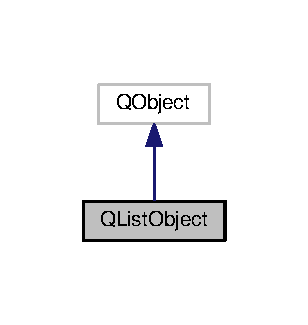
\includegraphics[width=148pt]{class_q_list_object__inherit__graph}
\end{center}
\end{figure}
\subsection*{Public Member Functions}
\begin{DoxyCompactItemize}
\item 
\hyperlink{class_q_list_object_a83076620d8a83ebb0d2b2a4a8bd84e38}{Q\+List\+Object} (Q\+Object $\ast$parent=0)
\begin{DoxyCompactList}\small\item\em This constructor can receive a parent. \end{DoxyCompactList}\item 
\hyperlink{class_q_list_object_a074ae68f366e150abacb1c4baa492bb6}{$\sim$\+Q\+List\+Object} ()
\item 
Q\+Object $\ast$ \hyperlink{class_q_list_object_a6f07490df1b1ba2ed37c7f322e12017b}{operator\mbox{[}$\,$\mbox{]}} (int index) const
\begin{DoxyCompactList}\small\item\em This is an operator overload and returns a Q\+Object given an specific index. \end{DoxyCompactList}\item 
int \hyperlink{class_q_list_object_a4ded55097ea08fa5781240883a591216}{size} () const
\begin{DoxyCompactList}\small\item\em This method returns the number of elements in this \hyperlink{class_q_list_object}{Q\+List\+Object}. \end{DoxyCompactList}\item 
void \hyperlink{class_q_list_object_ad5e960eabd3e9b7d49228ea7549a9bd7}{add} (Q\+Object $\ast$object)
\begin{DoxyCompactList}\small\item\em This method add a new Q\+Object to the list. \end{DoxyCompactList}\item 
void \hyperlink{class_q_list_object_af6bc1883142f976bfd3e82c9d0c030bb}{remove} (Q\+Object $\ast$object)
\begin{DoxyCompactList}\small\item\em This method remove and object from the list. \end{DoxyCompactList}\item 
bool \hyperlink{class_q_list_object_ad9d1f7e3c9f2563bcded31b02edc06fb}{get\+Auto\+Delete} () const
\begin{DoxyCompactList}\small\item\em get\+Auto\+Delete \end{DoxyCompactList}\item 
void \hyperlink{class_q_list_object_a6c30632fb46f8f7d404f77a9fea49bee}{set\+Auto\+Delete} (bool value)
\begin{DoxyCompactList}\small\item\em set\+Auto\+Delete \end{DoxyCompactList}\end{DoxyCompactItemize}


\subsection{Detailed Description}
The \hyperlink{class_q_list_object}{Q\+List\+Object} class is used to pass a list of object to a xhtml page. N\+O\+TE\+: Always when you need to pass a list of object to a xhtml page you will need to use this class, your class need to inherit from the Q\+Object class and all the methods needs to be in the public slots session. 

\subsection{Constructor \& Destructor Documentation}
\mbox{\Hypertarget{class_q_list_object_a83076620d8a83ebb0d2b2a4a8bd84e38}\label{class_q_list_object_a83076620d8a83ebb0d2b2a4a8bd84e38}} 
\index{Q\+List\+Object@{Q\+List\+Object}!Q\+List\+Object@{Q\+List\+Object}}
\index{Q\+List\+Object@{Q\+List\+Object}!Q\+List\+Object@{Q\+List\+Object}}
\subsubsection{\texorpdfstring{Q\+List\+Object()}{QListObject()}}
{\footnotesize\ttfamily \hyperlink{cppwebframework__global_8h_a7492e9498cbaf9cd17dbc2215d3a0e48}{C\+W\+F\+\_\+\+B\+E\+G\+I\+N\+\_\+\+N\+A\+M\+E\+S\+P\+A\+CE} Q\+List\+Object\+::\+Q\+List\+Object (\begin{DoxyParamCaption}\item[{Q\+Object $\ast$}]{parent = {\ttfamily 0} }\end{DoxyParamCaption})\hspace{0.3cm}{\ttfamily [explicit]}}



This constructor can receive a parent. 


\begin{DoxyParams}{Parameters}
{\em Q\+Object} & $\ast$parent \+: Parent. \\
\hline
\end{DoxyParams}
\mbox{\Hypertarget{class_q_list_object_a074ae68f366e150abacb1c4baa492bb6}\label{class_q_list_object_a074ae68f366e150abacb1c4baa492bb6}} 
\index{Q\+List\+Object@{Q\+List\+Object}!````~Q\+List\+Object@{$\sim$\+Q\+List\+Object}}
\index{````~Q\+List\+Object@{$\sim$\+Q\+List\+Object}!Q\+List\+Object@{Q\+List\+Object}}
\subsubsection{\texorpdfstring{$\sim$\+Q\+List\+Object()}{~QListObject()}}
{\footnotesize\ttfamily Q\+List\+Object\+::$\sim$\+Q\+List\+Object (\begin{DoxyParamCaption}{ }\end{DoxyParamCaption})}



\subsection{Member Function Documentation}
\mbox{\Hypertarget{class_q_list_object_ad5e960eabd3e9b7d49228ea7549a9bd7}\label{class_q_list_object_ad5e960eabd3e9b7d49228ea7549a9bd7}} 
\index{Q\+List\+Object@{Q\+List\+Object}!add@{add}}
\index{add@{add}!Q\+List\+Object@{Q\+List\+Object}}
\subsubsection{\texorpdfstring{add()}{add()}}
{\footnotesize\ttfamily void Q\+List\+Object\+::add (\begin{DoxyParamCaption}\item[{Q\+Object $\ast$}]{object }\end{DoxyParamCaption})}



This method add a new Q\+Object to the list. 


\begin{DoxyParams}{Parameters}
{\em Q\+Object} & $\ast$object \+: Object. \\
\hline
\end{DoxyParams}
\mbox{\Hypertarget{class_q_list_object_ad9d1f7e3c9f2563bcded31b02edc06fb}\label{class_q_list_object_ad9d1f7e3c9f2563bcded31b02edc06fb}} 
\index{Q\+List\+Object@{Q\+List\+Object}!get\+Auto\+Delete@{get\+Auto\+Delete}}
\index{get\+Auto\+Delete@{get\+Auto\+Delete}!Q\+List\+Object@{Q\+List\+Object}}
\subsubsection{\texorpdfstring{get\+Auto\+Delete()}{getAutoDelete()}}
{\footnotesize\ttfamily bool Q\+List\+Object\+::get\+Auto\+Delete (\begin{DoxyParamCaption}{ }\end{DoxyParamCaption}) const}



get\+Auto\+Delete 

\begin{DoxyReturn}{Returns}

\end{DoxyReturn}
\mbox{\Hypertarget{class_q_list_object_a6f07490df1b1ba2ed37c7f322e12017b}\label{class_q_list_object_a6f07490df1b1ba2ed37c7f322e12017b}} 
\index{Q\+List\+Object@{Q\+List\+Object}!operator\mbox{[}\mbox{]}@{operator[]}}
\index{operator\mbox{[}\mbox{]}@{operator[]}!Q\+List\+Object@{Q\+List\+Object}}
\subsubsection{\texorpdfstring{operator[]()}{operator[]()}}
{\footnotesize\ttfamily Q\+Object $\ast$ Q\+List\+Object\+::operator\mbox{[}$\,$\mbox{]} (\begin{DoxyParamCaption}\item[{int}]{index }\end{DoxyParamCaption}) const}



This is an operator overload and returns a Q\+Object given an specific index. 


\begin{DoxyParams}{Parameters}
{\em index} & \+: This is an integer value. \\
\hline
\end{DoxyParams}
\begin{DoxyReturn}{Returns}
Q\+Object $\ast$ 
\end{DoxyReturn}
\mbox{\Hypertarget{class_q_list_object_af6bc1883142f976bfd3e82c9d0c030bb}\label{class_q_list_object_af6bc1883142f976bfd3e82c9d0c030bb}} 
\index{Q\+List\+Object@{Q\+List\+Object}!remove@{remove}}
\index{remove@{remove}!Q\+List\+Object@{Q\+List\+Object}}
\subsubsection{\texorpdfstring{remove()}{remove()}}
{\footnotesize\ttfamily void Q\+List\+Object\+::remove (\begin{DoxyParamCaption}\item[{Q\+Object $\ast$}]{object }\end{DoxyParamCaption})}



This method remove and object from the list. 


\begin{DoxyParams}{Parameters}
{\em o} & \\
\hline
\end{DoxyParams}
\mbox{\Hypertarget{class_q_list_object_a6c30632fb46f8f7d404f77a9fea49bee}\label{class_q_list_object_a6c30632fb46f8f7d404f77a9fea49bee}} 
\index{Q\+List\+Object@{Q\+List\+Object}!set\+Auto\+Delete@{set\+Auto\+Delete}}
\index{set\+Auto\+Delete@{set\+Auto\+Delete}!Q\+List\+Object@{Q\+List\+Object}}
\subsubsection{\texorpdfstring{set\+Auto\+Delete()}{setAutoDelete()}}
{\footnotesize\ttfamily void Q\+List\+Object\+::set\+Auto\+Delete (\begin{DoxyParamCaption}\item[{bool}]{value }\end{DoxyParamCaption})}



set\+Auto\+Delete 


\begin{DoxyParams}{Parameters}
{\em value} & \\
\hline
\end{DoxyParams}
\mbox{\Hypertarget{class_q_list_object_a4ded55097ea08fa5781240883a591216}\label{class_q_list_object_a4ded55097ea08fa5781240883a591216}} 
\index{Q\+List\+Object@{Q\+List\+Object}!size@{size}}
\index{size@{size}!Q\+List\+Object@{Q\+List\+Object}}
\subsubsection{\texorpdfstring{size()}{size()}}
{\footnotesize\ttfamily int Q\+List\+Object\+::size (\begin{DoxyParamCaption}{ }\end{DoxyParamCaption}) const}



This method returns the number of elements in this \hyperlink{class_q_list_object}{Q\+List\+Object}. 

\begin{DoxyReturn}{Returns}
int 
\end{DoxyReturn}


The documentation for this class was generated from the following files\+:\begin{DoxyCompactItemize}
\item 
/home/herik/\+C\+P\+P\+Web\+Framework/\+C\+P\+P\+Web\+Framework/cwf/\hyperlink{qlistobject_8h}{qlistobject.\+h}\item 
/home/herik/\+C\+P\+P\+Web\+Framework/\+C\+P\+P\+Web\+Framework/cwf/\hyperlink{qlistobject_8cpp}{qlistobject.\+cpp}\end{DoxyCompactItemize}

\hypertarget{class_q_map_thread_safety}{}\section{Q\+Map\+Thread\+Safety$<$ Key, T $>$ Class Template Reference}
\label{class_q_map_thread_safety}\index{Q\+Map\+Thread\+Safety$<$ Key, T $>$@{Q\+Map\+Thread\+Safety$<$ Key, T $>$}}


The \mbox{\hyperlink{class_q_map_thread_safety}{Q\+Map\+Thread\+Safety}} class is a thread safe Q\+Map.  




{\ttfamily \#include $<$qmapthreadsafety.\+h$>$}

\subsection*{Public Types}
\begin{DoxyCompactItemize}
\item 
\mbox{\Hypertarget{class_q_map_thread_safety_a454c8af3f68e6d61aecaf1b918aa525b}\label{class_q_map_thread_safety_a454c8af3f68e6d61aecaf1b918aa525b}} 
typedef Q\+Map$<$ Key, T $>$\+::iterator {\bfseries iterator}
\item 
\mbox{\Hypertarget{class_q_map_thread_safety_aa58d8479729f72b33e305a4d0ca957bd}\label{class_q_map_thread_safety_aa58d8479729f72b33e305a4d0ca957bd}} 
typedef Q\+Map$<$ Key, T $>$\+::const\+\_\+iterator {\bfseries const\+\_\+iterator}
\end{DoxyCompactItemize}
\subsection*{Public Member Functions}
\begin{DoxyCompactItemize}
\item 
\mbox{\Hypertarget{class_q_map_thread_safety_a8b1bc71d8c92c4d01b6b3baae9787bb4}\label{class_q_map_thread_safety_a8b1bc71d8c92c4d01b6b3baae9787bb4}} 
{\bfseries Q\+Map\+Thread\+Safety} (std\+::initializer\+\_\+list$<$ std\+::pair$<$ Key, T $>$$>$ \&list)
\item 
\mbox{\Hypertarget{class_q_map_thread_safety_a368c8f4f05a48864209ab6ff5cf2f090}\label{class_q_map_thread_safety_a368c8f4f05a48864209ab6ff5cf2f090}} 
{\bfseries Q\+Map\+Thread\+Safety} (const Q\+Map$<$ Key, T $>$ \&other)
\item 
\mbox{\Hypertarget{class_q_map_thread_safety_a1335c04a2df7eda320f7a778854531fc}\label{class_q_map_thread_safety_a1335c04a2df7eda320f7a778854531fc}} 
{\bfseries Q\+Map\+Thread\+Safety} (const std\+::map$<$ Key, T $>$ \&other)
\item 
\mbox{\Hypertarget{class_q_map_thread_safety_a9aacfb2a81fb927546a222cbfd78000d}\label{class_q_map_thread_safety_a9aacfb2a81fb927546a222cbfd78000d}} 
{\bfseries Q\+Map\+Thread\+Safety} (Q\+Map$<$ Key, T $>$ \&\&other)
\item 
iterator \mbox{\hyperlink{class_q_map_thread_safety_ac197a5375913e4ac19910b9bc4191a95}{begin}} () const
\begin{DoxyCompactList}\small\item\em This method retuns the begin iterator. \end{DoxyCompactList}\item 
\mbox{\Hypertarget{class_q_map_thread_safety_aeddc5f7a55aebb3e93d78cf30a3dd2e1}\label{class_q_map_thread_safety_aeddc5f7a55aebb3e93d78cf30a3dd2e1}} 
const\+\_\+iterator {\bfseries cbegin} () const
\item 
\mbox{\Hypertarget{class_q_map_thread_safety_a199144509173057ede04d61f7294b266}\label{class_q_map_thread_safety_a199144509173057ede04d61f7294b266}} 
const\+\_\+iterator {\bfseries cend} () const
\item 
\mbox{\Hypertarget{class_q_map_thread_safety_a300f55a4c8e8ed3b5ccc2824dc18e60c}\label{class_q_map_thread_safety_a300f55a4c8e8ed3b5ccc2824dc18e60c}} 
const\+\_\+iterator {\bfseries const\+Begin} () const
\item 
\mbox{\Hypertarget{class_q_map_thread_safety_aa98a2af8cafc423c6bc6a04fec106b39}\label{class_q_map_thread_safety_aa98a2af8cafc423c6bc6a04fec106b39}} 
const\+\_\+iterator {\bfseries const\+End} () const
\item 
\mbox{\Hypertarget{class_q_map_thread_safety_ac364cabf8837a0b174016656b6bda81b}\label{class_q_map_thread_safety_ac364cabf8837a0b174016656b6bda81b}} 
const\+\_\+iterator {\bfseries const\+Find} (const Key \&key) const
\item 
bool \mbox{\hyperlink{class_q_map_thread_safety_acaafd9933cb391e27a81c26df712786b}{contains}} (const Key \&key) const
\begin{DoxyCompactList}\small\item\em This method checks if the map contains and specific element given a specific key. \end{DoxyCompactList}\item 
\mbox{\Hypertarget{class_q_map_thread_safety_a4542fc3dc112550bf8b0833338bfcaaf}\label{class_q_map_thread_safety_a4542fc3dc112550bf8b0833338bfcaaf}} 
int {\bfseries count} (const Key \&key) const
\item 
\mbox{\Hypertarget{class_q_map_thread_safety_a8adacf9b06525045bd79c909cea90f0a}\label{class_q_map_thread_safety_a8adacf9b06525045bd79c909cea90f0a}} 
int {\bfseries count} () const
\item 
\mbox{\Hypertarget{class_q_map_thread_safety_a5becb3980d1b35a27edde74f78ed43e2}\label{class_q_map_thread_safety_a5becb3980d1b35a27edde74f78ed43e2}} 
bool {\bfseries empty} () const
\item 
iterator \mbox{\hyperlink{class_q_map_thread_safety_a64a700a04a692176f00e119500dd1b23}{end}} ()
\begin{DoxyCompactList}\small\item\em This method retuns the end iterator. \end{DoxyCompactList}\item 
\mbox{\Hypertarget{class_q_map_thread_safety_aea999f181f31f0ac6bd01bcc016a673c}\label{class_q_map_thread_safety_aea999f181f31f0ac6bd01bcc016a673c}} 
Q\+Pair$<$ iterator, iterator $>$ {\bfseries equal\+\_\+range} (const Key \&key)
\item 
\mbox{\Hypertarget{class_q_map_thread_safety_a11c11617434ce781961ee8f722208d0e}\label{class_q_map_thread_safety_a11c11617434ce781961ee8f722208d0e}} 
iterator {\bfseries erase} (iterator pos)
\item 
\mbox{\Hypertarget{class_q_map_thread_safety_a3e4df3d688c99d259c6245a6f612c096}\label{class_q_map_thread_safety_a3e4df3d688c99d259c6245a6f612c096}} 
iterator {\bfseries find} (const Key \&key)
\item 
\mbox{\Hypertarget{class_q_map_thread_safety_a2564aae6f1946dfc48ae0576f4de0434}\label{class_q_map_thread_safety_a2564aae6f1946dfc48ae0576f4de0434}} 
const\+\_\+iterator {\bfseries find} (const Key \&key) const
\item 
\mbox{\Hypertarget{class_q_map_thread_safety_a3709dc412a794c75c4f678409324006f}\label{class_q_map_thread_safety_a3709dc412a794c75c4f678409324006f}} 
T \& {\bfseries first} ()
\item 
\mbox{\Hypertarget{class_q_map_thread_safety_ac2f2f58bb6a3dbd370134a96d3310222}\label{class_q_map_thread_safety_ac2f2f58bb6a3dbd370134a96d3310222}} 
const T \& {\bfseries first} () const
\item 
\mbox{\Hypertarget{class_q_map_thread_safety_ae1f69d7b72decd18f00f97d70e3daf88}\label{class_q_map_thread_safety_ae1f69d7b72decd18f00f97d70e3daf88}} 
const Key \& {\bfseries first\+Key} () const
\item 
iterator \mbox{\hyperlink{class_q_map_thread_safety_a156afe871591b26ce155da6ce6409ad6}{insert}} (const Key \&key, const T \&value)
\begin{DoxyCompactList}\small\item\em This method inserts a new key and value in the map. \end{DoxyCompactList}\item 
\mbox{\Hypertarget{class_q_map_thread_safety_a479e559360d2ba5471304b3dc9deb9dd}\label{class_q_map_thread_safety_a479e559360d2ba5471304b3dc9deb9dd}} 
iterator {\bfseries insert} (const\+\_\+iterator pos, const Key \&key, const T \&value)
\item 
\mbox{\Hypertarget{class_q_map_thread_safety_adb0bc3f6ee968de8b71a141bcc517d4c}\label{class_q_map_thread_safety_adb0bc3f6ee968de8b71a141bcc517d4c}} 
iterator {\bfseries insert\+Multi} (const Key \&key, const T \&value)
\item 
\mbox{\Hypertarget{class_q_map_thread_safety_a2dc915bd74285298d93eb17440587931}\label{class_q_map_thread_safety_a2dc915bd74285298d93eb17440587931}} 
bool {\bfseries is\+Empty} () const
\item 
\mbox{\Hypertarget{class_q_map_thread_safety_a51d0d694a419e2d0958b16f7089ab444}\label{class_q_map_thread_safety_a51d0d694a419e2d0958b16f7089ab444}} 
Q\+List$<$ Key $>$ {\bfseries keys} () const
\item 
\mbox{\Hypertarget{class_q_map_thread_safety_a721c6cae55a5c046a2fca6efc8fa49c3}\label{class_q_map_thread_safety_a721c6cae55a5c046a2fca6efc8fa49c3}} 
Q\+List$<$ Key $>$ {\bfseries keys} (const T \&value) const
\item 
\mbox{\Hypertarget{class_q_map_thread_safety_a87a87d963bc7624cc6330060d5a65f85}\label{class_q_map_thread_safety_a87a87d963bc7624cc6330060d5a65f85}} 
T \& {\bfseries last} ()
\item 
\mbox{\Hypertarget{class_q_map_thread_safety_a60bbb036a7cb0b05254a0171ad81e2db}\label{class_q_map_thread_safety_a60bbb036a7cb0b05254a0171ad81e2db}} 
const T \& {\bfseries last} () const
\item 
\mbox{\Hypertarget{class_q_map_thread_safety_a0589ec5e16479a92c0c50f86b32c1307}\label{class_q_map_thread_safety_a0589ec5e16479a92c0c50f86b32c1307}} 
iterator {\bfseries lower\+Bound} (const Key \&key)
\item 
\mbox{\Hypertarget{class_q_map_thread_safety_a21e8f53194d173f6cedb8d60a86a4a19}\label{class_q_map_thread_safety_a21e8f53194d173f6cedb8d60a86a4a19}} 
const\+\_\+iterator {\bfseries lower\+Bound} (const Key \&key) const
\item 
int \mbox{\hyperlink{class_q_map_thread_safety_a91e703ad03572023876108c2b7bc3540}{remove}} (const Key \&key)
\begin{DoxyCompactList}\small\item\em This method removes a specific element given a specific key. \end{DoxyCompactList}\item 
\mbox{\Hypertarget{class_q_map_thread_safety_a0331b4ea9616aa81d1ede4066113c35b}\label{class_q_map_thread_safety_a0331b4ea9616aa81d1ede4066113c35b}} 
int {\bfseries size} () const
\item 
\mbox{\Hypertarget{class_q_map_thread_safety_addcefa9985e7fa96939eca2a8e2b1fcc}\label{class_q_map_thread_safety_addcefa9985e7fa96939eca2a8e2b1fcc}} 
void {\bfseries swap} (Q\+Map$<$ Key, T $>$ \&other)
\item 
\mbox{\Hypertarget{class_q_map_thread_safety_a03f5056559f4d0f2500ddcb8ddf55098}\label{class_q_map_thread_safety_a03f5056559f4d0f2500ddcb8ddf55098}} 
T {\bfseries take} (const Key \&key)
\item 
\mbox{\Hypertarget{class_q_map_thread_safety_ad145bbf62ebe8d796ed1a8216bfbe69d}\label{class_q_map_thread_safety_ad145bbf62ebe8d796ed1a8216bfbe69d}} 
std\+::map$<$ Key, T $>$ {\bfseries to\+Std\+Map} () const
\item 
\mbox{\Hypertarget{class_q_map_thread_safety_a8d3498ec21684e0c221ce2eddb437ecd}\label{class_q_map_thread_safety_a8d3498ec21684e0c221ce2eddb437ecd}} 
Q\+List$<$ Key $>$ {\bfseries unique\+Keys} () const
\item 
\mbox{\Hypertarget{class_q_map_thread_safety_a784205cd91eaed840f8d2554a07d3c22}\label{class_q_map_thread_safety_a784205cd91eaed840f8d2554a07d3c22}} 
Q\+Map$<$ Key, T $>$ \& {\bfseries unite} (const Q\+Map$<$ Key, T $>$ \&other)
\item 
\mbox{\Hypertarget{class_q_map_thread_safety_aa43810522d484b2364777e0701486109}\label{class_q_map_thread_safety_aa43810522d484b2364777e0701486109}} 
iterator {\bfseries upper\+Bound} (const Key \&key)
\item 
\mbox{\Hypertarget{class_q_map_thread_safety_a24c3c21d5d756ff3592a3139a9710995}\label{class_q_map_thread_safety_a24c3c21d5d756ff3592a3139a9710995}} 
const\+\_\+iterator {\bfseries upper\+Bound} (const Key \&key) const
\item 
\mbox{\Hypertarget{class_q_map_thread_safety_a3c5caec402261554fd4d73e36e9ca6bc}\label{class_q_map_thread_safety_a3c5caec402261554fd4d73e36e9ca6bc}} 
const T {\bfseries value} (const Key \&key, const T \&default\+Value=T()) const
\item 
\mbox{\Hypertarget{class_q_map_thread_safety_a6395316e7fec3faea0dcf150a3dab897}\label{class_q_map_thread_safety_a6395316e7fec3faea0dcf150a3dab897}} 
Q\+List$<$ T $>$ {\bfseries values} () const
\item 
\mbox{\Hypertarget{class_q_map_thread_safety_afffdf1fc9bd98f9bfede07549533da53}\label{class_q_map_thread_safety_afffdf1fc9bd98f9bfede07549533da53}} 
Q\+List$<$ T $>$ {\bfseries values} (const Key \&key) const
\item 
\mbox{\Hypertarget{class_q_map_thread_safety_a48d648aa531db7c8ecd7f2efe2153707}\label{class_q_map_thread_safety_a48d648aa531db7c8ecd7f2efe2153707}} 
bool {\bfseries operator!=} (const Q\+Map$<$ Key, T $>$ \&other) const
\item 
\mbox{\Hypertarget{class_q_map_thread_safety_af33ed0b71924a4281f4f25bf5eda1cfd}\label{class_q_map_thread_safety_af33ed0b71924a4281f4f25bf5eda1cfd}} 
Q\+Map$<$ Key, T $>$ \& {\bfseries operator=} (const Q\+Map$<$ Key, T $>$ \&other)
\item 
\mbox{\Hypertarget{class_q_map_thread_safety_a0845272b1bc863dd153607e63efa839d}\label{class_q_map_thread_safety_a0845272b1bc863dd153607e63efa839d}} 
Q\+Map$<$ Key, T $>$ \& {\bfseries operator=} (Q\+Map$<$ Key, T $>$ \&\&other)
\item 
\mbox{\Hypertarget{class_q_map_thread_safety_a343008196414aa4fe66ff2de5ca29986}\label{class_q_map_thread_safety_a343008196414aa4fe66ff2de5ca29986}} 
bool {\bfseries operator==} (const Q\+Map$<$ Key, T $>$ \&other) const
\item 
\mbox{\Hypertarget{class_q_map_thread_safety_ac9c974843e1bbf7f4bff2acc4f88f300}\label{class_q_map_thread_safety_ac9c974843e1bbf7f4bff2acc4f88f300}} 
T \& {\bfseries operator\mbox{[}$\,$\mbox{]}} (const Key \&key)
\item 
const T \mbox{\hyperlink{class_q_map_thread_safety_a0cdacf0e7048c4ef7e0960a371c32668}{operator\mbox{[}$\,$\mbox{]}}} (const Key \&key) const
\begin{DoxyCompactList}\small\item\em This method is an overload of the operator \mbox{[}\mbox{]} and returns a value given a specific key. \end{DoxyCompactList}\end{DoxyCompactItemize}


\subsection{Detailed Description}
\subsubsection*{template$<$typename Key, typename T$>$\newline
class Q\+Map\+Thread\+Safety$<$ Key, T $>$}

The \mbox{\hyperlink{class_q_map_thread_safety}{Q\+Map\+Thread\+Safety}} class is a thread safe Q\+Map. 

\subsection{Member Function Documentation}
\mbox{\Hypertarget{class_q_map_thread_safety_ac197a5375913e4ac19910b9bc4191a95}\label{class_q_map_thread_safety_ac197a5375913e4ac19910b9bc4191a95}} 
\index{Q\+Map\+Thread\+Safety@{Q\+Map\+Thread\+Safety}!begin@{begin}}
\index{begin@{begin}!Q\+Map\+Thread\+Safety@{Q\+Map\+Thread\+Safety}}
\subsubsection{\texorpdfstring{begin()}{begin()}}
{\footnotesize\ttfamily template$<$typename Key, typename T$>$ \\
iterator \mbox{\hyperlink{class_q_map_thread_safety}{Q\+Map\+Thread\+Safety}}$<$ Key, T $>$\+::begin (\begin{DoxyParamCaption}{ }\end{DoxyParamCaption}) const\hspace{0.3cm}{\ttfamily [inline]}}



This method retuns the begin iterator. 

\begin{DoxyReturn}{Returns}
iterator 
\end{DoxyReturn}
\mbox{\Hypertarget{class_q_map_thread_safety_acaafd9933cb391e27a81c26df712786b}\label{class_q_map_thread_safety_acaafd9933cb391e27a81c26df712786b}} 
\index{Q\+Map\+Thread\+Safety@{Q\+Map\+Thread\+Safety}!contains@{contains}}
\index{contains@{contains}!Q\+Map\+Thread\+Safety@{Q\+Map\+Thread\+Safety}}
\subsubsection{\texorpdfstring{contains()}{contains()}}
{\footnotesize\ttfamily template$<$typename Key, typename T$>$ \\
bool \mbox{\hyperlink{class_q_map_thread_safety}{Q\+Map\+Thread\+Safety}}$<$ Key, T $>$\+::contains (\begin{DoxyParamCaption}\item[{const Key \&}]{key }\end{DoxyParamCaption}) const\hspace{0.3cm}{\ttfamily [inline]}}



This method checks if the map contains and specific element given a specific key. 


\begin{DoxyParams}{Parameters}
{\em key} & \+: This represents the key that you want to find. \\
\hline
\end{DoxyParams}
\begin{DoxyReturn}{Returns}
returns true if find the key and false if not find. 
\end{DoxyReturn}
\mbox{\Hypertarget{class_q_map_thread_safety_a64a700a04a692176f00e119500dd1b23}\label{class_q_map_thread_safety_a64a700a04a692176f00e119500dd1b23}} 
\index{Q\+Map\+Thread\+Safety@{Q\+Map\+Thread\+Safety}!end@{end}}
\index{end@{end}!Q\+Map\+Thread\+Safety@{Q\+Map\+Thread\+Safety}}
\subsubsection{\texorpdfstring{end()}{end()}}
{\footnotesize\ttfamily template$<$typename Key, typename T$>$ \\
iterator \mbox{\hyperlink{class_q_map_thread_safety}{Q\+Map\+Thread\+Safety}}$<$ Key, T $>$\+::end (\begin{DoxyParamCaption}{ }\end{DoxyParamCaption})\hspace{0.3cm}{\ttfamily [inline]}}



This method retuns the end iterator. 

\begin{DoxyReturn}{Returns}
iterator 
\end{DoxyReturn}
\mbox{\Hypertarget{class_q_map_thread_safety_a156afe871591b26ce155da6ce6409ad6}\label{class_q_map_thread_safety_a156afe871591b26ce155da6ce6409ad6}} 
\index{Q\+Map\+Thread\+Safety@{Q\+Map\+Thread\+Safety}!insert@{insert}}
\index{insert@{insert}!Q\+Map\+Thread\+Safety@{Q\+Map\+Thread\+Safety}}
\subsubsection{\texorpdfstring{insert()}{insert()}}
{\footnotesize\ttfamily template$<$typename Key, typename T$>$ \\
iterator \mbox{\hyperlink{class_q_map_thread_safety}{Q\+Map\+Thread\+Safety}}$<$ Key, T $>$\+::insert (\begin{DoxyParamCaption}\item[{const Key \&}]{key,  }\item[{const T \&}]{value }\end{DoxyParamCaption})\hspace{0.3cm}{\ttfamily [inline]}}



This method inserts a new key and value in the map. 


\begin{DoxyParams}{Parameters}
{\em key} & \+: This represents the key that will be insert. \\
\hline
{\em value} & \+: This represents the value that will be insert. \\
\hline
\end{DoxyParams}
\mbox{\Hypertarget{class_q_map_thread_safety_a0cdacf0e7048c4ef7e0960a371c32668}\label{class_q_map_thread_safety_a0cdacf0e7048c4ef7e0960a371c32668}} 
\index{Q\+Map\+Thread\+Safety@{Q\+Map\+Thread\+Safety}!operator\mbox{[}\mbox{]}@{operator[]}}
\index{operator\mbox{[}\mbox{]}@{operator[]}!Q\+Map\+Thread\+Safety@{Q\+Map\+Thread\+Safety}}
\subsubsection{\texorpdfstring{operator[]()}{operator[]()}}
{\footnotesize\ttfamily template$<$typename Key, typename T$>$ \\
const T \mbox{\hyperlink{class_q_map_thread_safety}{Q\+Map\+Thread\+Safety}}$<$ Key, T $>$\+::operator\mbox{[}$\,$\mbox{]} (\begin{DoxyParamCaption}\item[{const Key \&}]{key }\end{DoxyParamCaption}) const\hspace{0.3cm}{\ttfamily [inline]}}



This method is an overload of the operator \mbox{[}\mbox{]} and returns a value given a specific key. 


\begin{DoxyParams}{Parameters}
{\em key} & \+: This represents the key that you want to find. \\
\hline
\end{DoxyParams}
\begin{DoxyReturn}{Returns}
T 
\end{DoxyReturn}
\mbox{\Hypertarget{class_q_map_thread_safety_a91e703ad03572023876108c2b7bc3540}\label{class_q_map_thread_safety_a91e703ad03572023876108c2b7bc3540}} 
\index{Q\+Map\+Thread\+Safety@{Q\+Map\+Thread\+Safety}!remove@{remove}}
\index{remove@{remove}!Q\+Map\+Thread\+Safety@{Q\+Map\+Thread\+Safety}}
\subsubsection{\texorpdfstring{remove()}{remove()}}
{\footnotesize\ttfamily template$<$typename Key, typename T$>$ \\
int \mbox{\hyperlink{class_q_map_thread_safety}{Q\+Map\+Thread\+Safety}}$<$ Key, T $>$\+::remove (\begin{DoxyParamCaption}\item[{const Key \&}]{key }\end{DoxyParamCaption})\hspace{0.3cm}{\ttfamily [inline]}}



This method removes a specific element given a specific key. 


\begin{DoxyParams}{Parameters}
{\em key} & \+: This represents the key that will be insert. \\
\hline
\end{DoxyParams}
\begin{DoxyReturn}{Returns}
int 
\end{DoxyReturn}


The documentation for this class was generated from the following file\+:\begin{DoxyCompactItemize}
\item 
C\+:/\+C\+P\+P\+Web\+Framework/\+C\+P\+P\+Web\+Framework/cwf/qmapthreadsafety.\+h\end{DoxyCompactItemize}

\hypertarget{class_request}{}\section{Request Class Reference}
\label{class_request}\index{Request@{Request}}


The \hyperlink{class_request}{Request} class holds all information about a http request.  




{\ttfamily \#include $<$request.\+h$>$}



Inheritance diagram for Request\+:
% FIG 0
\subsection*{Public Member Functions}
\begin{DoxyCompactItemize}
\item 
\mbox{\Hypertarget{class_request_a5dbe3045d76139502b0c0db5c67ea900}\label{class_request_a5dbe3045d76139502b0c0db5c67ea900}} 
\hyperlink{class_request_a5dbe3045d76139502b0c0db5c67ea900}{Request} (Q\+Tcp\+Socket \&socket, \hyperlink{class_q_map_thread_safety}{Q\+Map\+Thread\+Safety}$<$ Q\+String, \hyperlink{class_session}{Session} $\ast$$>$ \&sessions, const \hyperlink{class_configuration}{Configuration} \&configuration)
\begin{DoxyCompactList}\small\item\em This constructor needs to receive a reference to a Q\+Tcp\+Socket and Q\+Byte\+Array. The parameter parent is optional. N\+O\+TE\+: The \hyperlink{class_cpp_web_server}{Cpp\+Web\+Server} is responsable to create the Q\+Tcp\+Socket, and the \hyperlink{class_http_read_request}{Http\+Read\+Request} is responsable to create a \hyperlink{class_http_read_request}{Http\+Read\+Request} and a \hyperlink{class_response}{Response}. \end{DoxyCompactList}\item 
\mbox{\Hypertarget{class_request_a4d57c725686701f773eb3630630a7ea2}\label{class_request_a4d57c725686701f773eb3630630a7ea2}} 
virtual \hyperlink{class_request_a4d57c725686701f773eb3630630a7ea2}{$\sim$\+Request} ()
\begin{DoxyCompactList}\small\item\em Destroys dynamically allocated resources. \end{DoxyCompactList}\item 
\mbox{\Hypertarget{class_request_afe81be45f2fffc0e4baf2830278b8c94}\label{class_request_afe81be45f2fffc0e4baf2830278b8c94}} 
void \hyperlink{class_request_afe81be45f2fffc0e4baf2830278b8c94}{add\+Attribute} (const Q\+String \&name, Q\+Object $\ast$value) noexcept
\begin{DoxyCompactList}\small\item\em This method add an attribute that will be passed to a xhtml page. The object can be processed within a page using xhtml C\+S\+TL. For this to be possible the object must inherit from Q\+Object and methods and must be in session \char`\"{}public slots\char`\"{}. \end{DoxyCompactList}\item 
\mbox{\Hypertarget{class_request_affe1bd704eaad1077e5577d0f8a22392}\label{class_request_affe1bd704eaad1077e5577d0f8a22392}} 
Q\+Map$<$ Q\+String, Q\+Object $\ast$ $>$ \hyperlink{class_request_affe1bd704eaad1077e5577d0f8a22392}{get\+Attributes} () const noexcept
\begin{DoxyCompactList}\small\item\em This method returns all the attributes of a \hyperlink{class_http_read_request}{Http\+Read\+Request}. \end{DoxyCompactList}\item 
\mbox{\Hypertarget{class_request_ab4d1136eebec4011c5512f77dd5e00a2}\label{class_request_ab4d1136eebec4011c5512f77dd5e00a2}} 
const Q\+Object $\ast$ \hyperlink{class_request_ab4d1136eebec4011c5512f77dd5e00a2}{get\+Attribute} (const Q\+String \&name) const noexcept
\begin{DoxyCompactList}\small\item\em This method returns a specific object given its name. \end{DoxyCompactList}\item 
\mbox{\Hypertarget{class_request_a284909aadbbfd8f76472f8ebaf4ef16e}\label{class_request_a284909aadbbfd8f76472f8ebaf4ef16e}} 
const Q\+Byte\+Array \hyperlink{class_request_a284909aadbbfd8f76472f8ebaf4ef16e}{get\+Body} () const noexcept
\begin{DoxyCompactList}\small\item\em Returns the request body. \end{DoxyCompactList}\item 
\mbox{\Hypertarget{class_request_acb4c1802fbd8cf14183c231ebb586288}\label{class_request_acb4c1802fbd8cf14183c231ebb586288}} 
Q\+Json\+Object \hyperlink{class_request_acb4c1802fbd8cf14183c231ebb586288}{body\+To\+Json\+Object} () const noexcept
\begin{DoxyCompactList}\small\item\em Tries returns the body of the converted request to Q\+Json\+Object. \end{DoxyCompactList}\item 
\mbox{\Hypertarget{class_request_a933c1581ec12d55a0b307c4060d5e127}\label{class_request_a933c1581ec12d55a0b307c4060d5e127}} 
Q\+Json\+Array \hyperlink{class_request_a933c1581ec12d55a0b307c4060d5e127}{body\+To\+Json\+Array} () const noexcept
\begin{DoxyCompactList}\small\item\em Tries returns the body of the converted request to Q\+Json\+Array. \end{DoxyCompactList}\item 
\hyperlink{class_request_dispatcher}{Request\+Dispatcher} \& \hyperlink{class_request_a595822f6e39bf04930f9ad580a5ba34c}{get\+Request\+Dispatcher} (const Q\+String \&page)
\begin{DoxyCompactList}\small\item\em This method returns a request\+Dispatcher given an specific page. \end{DoxyCompactList}\item 
Q\+Byte\+Array \hyperlink{class_request_a975ffb8f0b6aa08879ffecb50d9bb289}{get\+Protocol} () const noexcept
\begin{DoxyCompactList}\small\item\em This method returns the http protocol. \end{DoxyCompactList}\item 
\mbox{\Hypertarget{class_request_a4a1aa80b942621b9bb12f3eca47a415b}\label{class_request_a4a1aa80b942621b9bb12f3eca47a415b}} 
void \hyperlink{class_request_a4a1aa80b942621b9bb12f3eca47a415b}{clear\+Attributes} ()
\begin{DoxyCompactList}\small\item\em This method will clear all the attributes. \end{DoxyCompactList}\item 
void \hyperlink{class_request_a526593ca8b89c6871a36fefb0f2cde1a}{set\+Http\+Parser} (\hyperlink{class_http_parser}{Http\+Parser} \&http\+Parser) noexcept
\begin{DoxyCompactList}\small\item\em This method set the \hyperlink{class_http_parser}{Http\+Parser}. \end{DoxyCompactList}\item 
\hyperlink{class_http_parser}{Http\+Parser} \& \hyperlink{class_request_ac593ca2abd88c9e21238a37da8c707f6}{get\+Http\+Parser} () const
\begin{DoxyCompactList}\small\item\em This method returns the \hyperlink{class_http_parser}{Http\+Parser}. \end{DoxyCompactList}\item 
Q\+Byte\+Array \hyperlink{class_request_a48d3b2a3579011b0599e721fdb867b27}{get\+Request\+U\+RL} () const noexcept
\begin{DoxyCompactList}\small\item\em This method returns the requested url. \end{DoxyCompactList}\item 
Q\+Byte\+Array \hyperlink{class_request_aa5f623afcbe306d552a495156e3bb9c1}{get\+Request\+U\+RI} () const noexcept
\begin{DoxyCompactList}\small\item\em This method returns the requested url. \end{DoxyCompactList}\item 
\mbox{\Hypertarget{class_request_a004a1262148d077d2de9a9855f5f7ef3}\label{class_request_a004a1262148d077d2de9a9855f5f7ef3}} 
\hyperlink{class_session}{Session} \& \hyperlink{class_request_a004a1262148d077d2de9a9855f5f7ef3}{get\+Session} ()
\begin{DoxyCompactList}\small\item\em This method returns the user\textquotesingle{}s session. \end{DoxyCompactList}\item 
void \hyperlink{class_request_ab11b66e85291c653579fbba30bfa1a70}{set\+Session} (\hyperlink{class_session}{Session} \&session) noexcept
\begin{DoxyCompactList}\small\item\em This method set the user\textquotesingle{}s session. \end{DoxyCompactList}\item 
Q\+Byte\+Array \hyperlink{class_request_a0a78d7b29f1c0d96f101df866c82cef5}{get\+Parameter} (const Q\+Byte\+Array \&name) const noexcept
\begin{DoxyCompactList}\small\item\em This method returns the most recent parameter from a request given an specific name. \end{DoxyCompactList}\item 
Q\+Byte\+Array\+List \hyperlink{class_request_a46c49de1519d33ee2ff3cbe5a2874fc9}{get\+Parameters} (const Q\+Byte\+Array \&name) const noexcept
\begin{DoxyCompactList}\small\item\em This method returns the parameters from a request given an specific name. \end{DoxyCompactList}\item 
Q\+Tcp\+Socket \& \hyperlink{class_request_a0469d7af31664f37234397ce2cc46012}{get\+Socket} () const noexcept
\begin{DoxyCompactList}\small\item\em This method returns a reference to the current socket. \end{DoxyCompactList}\item 
Q\+String \hyperlink{class_request_ad87c576630126d44838da46c18a90e01}{get\+Path} () const noexcept
\begin{DoxyCompactList}\small\item\em This method returns the path. \end{DoxyCompactList}\item 
Q\+Multi\+Map$<$ Q\+Byte\+Array, Q\+Byte\+Array $>$ \hyperlink{class_request_a61e5ed8f40ac13d028e27fda8695dace}{get\+Uploaded\+Files} () const noexcept
\begin{DoxyCompactList}\small\item\em This method returns all the files that the user has sent. \end{DoxyCompactList}\item 
void \hyperlink{class_request_a934d83fe6fe62aba36a625b6edad8d65}{fill\+Q\+Object} (Q\+Object $\ast$object)
\begin{DoxyCompactList}\small\item\em Fill a Q\+Object using parameters of a H\+T\+TP message. \end{DoxyCompactList}\end{DoxyCompactItemize}
\subsection*{Friends}
\begin{DoxyCompactItemize}
\item 
\mbox{\Hypertarget{class_request_a4d54f5003e07e218070a449c22a52c7c}\label{class_request_a4d54f5003e07e218070a449c22a52c7c}} 
class {\bfseries Http\+Read\+Request}
\item 
\mbox{\Hypertarget{class_request_ae82f2dbbf52e70637edba766141fd80e}\label{class_request_ae82f2dbbf52e70637edba766141fd80e}} 
class {\bfseries Request\+Dispatcher}
\end{DoxyCompactItemize}


\subsection{Detailed Description}
The \hyperlink{class_request}{Request} class holds all information about a http request. 

\subsection{Member Function Documentation}
\mbox{\Hypertarget{class_request_a934d83fe6fe62aba36a625b6edad8d65}\label{class_request_a934d83fe6fe62aba36a625b6edad8d65}} 
\index{Request@{Request}!fill\+Q\+Object@{fill\+Q\+Object}}
\index{fill\+Q\+Object@{fill\+Q\+Object}!Request@{Request}}
\subsubsection{\texorpdfstring{fill\+Q\+Object()}{fillQObject()}}
{\footnotesize\ttfamily void Request\+::fill\+Q\+Object (\begin{DoxyParamCaption}\item[{Q\+Object $\ast$}]{object }\end{DoxyParamCaption})}



Fill a Q\+Object using parameters of a H\+T\+TP message. 


\begin{DoxyParams}{Parameters}
{\em Q\+Object} & $\ast$object \+: Object to be filled. \\
\hline
\end{DoxyParams}
\begin{DoxyParagraph}{Example}

\begin{DoxyCode}
\textcolor{comment}{//----------------bmi.view----------------}

<?xml version=\textcolor{stringliteral}{"1.0"} encoding=\textcolor{stringliteral}{"iso-8859-1"} ?>
<html>
     <head>
         <title>Body Mass Index (BMI)</title>
     </head>
     <body>
         <form method=\textcolor{stringliteral}{"POST"} action=\textcolor{stringliteral}{"/bmi"}>
             Name<br/><input type=\textcolor{stringliteral}{"text"} name=\textcolor{stringliteral}{"name"}/><br/>
             Mass(KG)<br/><input type=\textcolor{stringliteral}{"text"} name=\textcolor{stringliteral}{"mass"}/><br/>
             Height(m)<br/><input type=\textcolor{stringliteral}{"text"} name=\textcolor{stringliteral}{"height"}/><br/><br/>
             <input type=\textcolor{stringliteral}{"submit"} name=\textcolor{stringliteral}{"submit"} value=\textcolor{stringliteral}{"Calculate"}/>
         </form>
     </body>
 </html>

\textcolor{comment}{//----------------bmiresults.view----------------}

<?xml version=\textcolor{stringliteral}{"1.0"} encoding=\textcolor{stringliteral}{"iso-8859-1"} ?>
<html>
     <head>
         <title>Body Mass Index (BMI) - Results</title>
     </head>
     <body>
         Name: <out value=\textcolor{stringliteral}{"#\{user.getName\}"}/><br/>
         Mass(KG): <out value=\textcolor{stringliteral}{"#\{user.getMass\}"}/><br/>
         Height(m): <out value=\textcolor{stringliteral}{"#\{user.getHeight\}"}/><br/>
         BMI: <out value=\textcolor{stringliteral}{"#\{user.getBmi\}"}/><br/>
         Category: <out value=\textcolor{stringliteral}{"#\{user.getCategory\}"}/>
     </body>
</html>

\textcolor{comment}{//----------------user.h----------------}

#ifndef USER\_H
#define USER\_H

#include <QObject>
#include <QString>

class User : public QObject
\{
    Q\_OBJECT
\textcolor{keyword}{private}:
    QString name;
    QString category;
    \textcolor{keywordtype}{double} mass = 0;
    \textcolor{keywordtype}{double} height = 0;
    \textcolor{keywordtype}{double} bmi = 0;
\textcolor{keyword}{public}:
    \textcolor{keyword}{explicit} User(QObject *parent = 0) : QObject(parent)
    \{
    \}
\textcolor{keyword}{public} slots:
    QString getName()\textcolor{keyword}{ const}
\textcolor{keyword}{    }\{
        \textcolor{keywordflow}{return} name;
    \}
    \textcolor{keywordtype}{void} setName(\textcolor{keyword}{const} QString &value)
    \{
        name = value;
    \}
    QString getCategory()\textcolor{keyword}{ const}
\textcolor{keyword}{    }\{
        \textcolor{keywordflow}{return} category;
    \}
    \textcolor{keywordtype}{double} getMass()\textcolor{keyword}{ const}
\textcolor{keyword}{    }\{
        \textcolor{keywordflow}{return} mass;
    \}
    \textcolor{keywordtype}{void} setMass(\textcolor{keywordtype}{double} value)
    \{
        mass = value;
    \}
    \textcolor{keywordtype}{double} getHeight()\textcolor{keyword}{ const}
\textcolor{keyword}{    }\{
        \textcolor{keywordflow}{return} height;
    \}
    \textcolor{keywordtype}{void} setHeight(\textcolor{keywordtype}{double} value)
    \{
        height = value;
    \}
    \textcolor{keywordtype}{double} getBmi()
    \{
        bmi = height != 0 ? mass / (height * height) : 0;

        \textcolor{keywordflow}{if}(bmi <= 15)
        \{
            category = \textcolor{stringliteral}{"Very severely underweight"};
        \}
        \textcolor{keywordflow}{else} \textcolor{keywordflow}{if}(bmi > 15 && bmi <= 16)
        \{
            category = \textcolor{stringliteral}{"Severely underweight"};
        \}
        \textcolor{keywordflow}{else} \textcolor{keywordflow}{if}(bmi > 16 && bmi <= 18.5)
        \{
            category = \textcolor{stringliteral}{"Underweight"};
        \}
        \textcolor{keywordflow}{else} \textcolor{keywordflow}{if}(bmi > 18.5 && bmi <= 25)
        \{
            category = \textcolor{stringliteral}{"Normal (healthy weight)"};
        \}
        \textcolor{keywordflow}{else} \textcolor{keywordflow}{if}(bmi > 25 && bmi <= 30)
        \{
            category = \textcolor{stringliteral}{"Overweight"};
        \}
        \textcolor{keywordflow}{else} \textcolor{keywordflow}{if}(bmi > 30 && bmi <= 35)
        \{
            category = \textcolor{stringliteral}{"Obese Class I (Moderately obese)"};
        \}
        \textcolor{keywordflow}{else} \textcolor{keywordflow}{if}(bmi > 35 && bmi <= 40)
        \{
            category = \textcolor{stringliteral}{"Obese Class II (Severely obese)"};
        \}
        \textcolor{keywordflow}{else}
        \{
            category = \textcolor{stringliteral}{"Obese Class III (Very severely obese)"};
        \}

        \textcolor{keywordflow}{return} bmi;
    \}
\};

\textcolor{preprocessor}{#endif // USER\_H}

\textcolor{comment}{//----------------bmicontroller.h----------------}

\textcolor{preprocessor}{#ifndef BMICONTROLLER\_H}
\textcolor{preprocessor}{#define BMICONTROLLER\_H}

\textcolor{preprocessor}{#include "cwf/controller.h"}
\textcolor{preprocessor}{#include "cwf/request.h"}
\textcolor{preprocessor}{#include "cwf/response.h"}
\textcolor{preprocessor}{#include "entities/user.h"}

\textcolor{keyword}{class }BmiController : \textcolor{keyword}{public} CWF::Controller
\{
\textcolor{keyword}{public}:
    \textcolor{keywordtype}{void} doGet(CWF::Request &request, CWF::Response &response)\textcolor{keyword}{ override}
\textcolor{keyword}{    }\{
        request.getRequestDispatcher(\textcolor{stringliteral}{"/pages/bmi"}).forward(request, response);
    \}
    \textcolor{keywordtype}{void} doPost(CWF::Request &request, CWF::Response &response)\textcolor{keyword}{ override}
\textcolor{keyword}{    }\{
        User user;
        request.fillQObject(&user);
        request.addAttribute(\textcolor{stringliteral}{"user"}, &user);
        request.getRequestDispatcher(\textcolor{stringliteral}{"/pages/bmiresults.view"}).forward(request, response);
    \}
\};

\textcolor{preprocessor}{#endif // BMICONTROLLER\_H}

\textcolor{comment}{//----------------main.cpp----------------}

\textcolor{preprocessor}{#include <QCoreApplication>}
\textcolor{preprocessor}{#include <cwf/cppwebapplication.h>}
\textcolor{preprocessor}{#include <controllers/bmicontroller.h>}

\textcolor{keywordtype}{int} main(\textcolor{keywordtype}{int} argc, \textcolor{keywordtype}{char} *argv[])
\{
    CWF::CppWebApplication server(argc, argv, \textcolor{stringliteral}{"PATH\_TO\_SERVER\_FOLDER"});

    server.addUrlController<BmiController>(\textcolor{stringliteral}{"/bmi"});

    \textcolor{keywordflow}{return} server.start();
\}
\end{DoxyCode}
 
\end{DoxyParagraph}
\mbox{\Hypertarget{class_request_ac593ca2abd88c9e21238a37da8c707f6}\label{class_request_ac593ca2abd88c9e21238a37da8c707f6}} 
\index{Request@{Request}!get\+Http\+Parser@{get\+Http\+Parser}}
\index{get\+Http\+Parser@{get\+Http\+Parser}!Request@{Request}}
\subsubsection{\texorpdfstring{get\+Http\+Parser()}{getHttpParser()}}
{\footnotesize\ttfamily \hyperlink{class_http_parser}{Http\+Parser}\& Request\+::get\+Http\+Parser (\begin{DoxyParamCaption}{ }\end{DoxyParamCaption}) const\hspace{0.3cm}{\ttfamily [inline]}}



This method returns the \hyperlink{class_http_parser}{Http\+Parser}. 

\begin{DoxyReturn}{Returns}
\hyperlink{class_http_parser}{Http\+Parser} 
\end{DoxyReturn}
\mbox{\Hypertarget{class_request_a0a78d7b29f1c0d96f101df866c82cef5}\label{class_request_a0a78d7b29f1c0d96f101df866c82cef5}} 
\index{Request@{Request}!get\+Parameter@{get\+Parameter}}
\index{get\+Parameter@{get\+Parameter}!Request@{Request}}
\subsubsection{\texorpdfstring{get\+Parameter()}{getParameter()}}
{\footnotesize\ttfamily Q\+Byte\+Array Request\+::get\+Parameter (\begin{DoxyParamCaption}\item[{const Q\+Byte\+Array \&}]{name }\end{DoxyParamCaption}) const\hspace{0.3cm}{\ttfamily [inline]}, {\ttfamily [noexcept]}}



This method returns the most recent parameter from a request given an specific name. 


\begin{DoxyParams}{Parameters}
{\em name} & \+: This is a reference to a Q\+Byte\+Array. \\
\hline
{\em decode} & \+: If true, decode the parameter. \\
\hline
\end{DoxyParams}
\begin{DoxyReturn}{Returns}
Q\+Byte\+Array 
\end{DoxyReturn}
\mbox{\Hypertarget{class_request_a46c49de1519d33ee2ff3cbe5a2874fc9}\label{class_request_a46c49de1519d33ee2ff3cbe5a2874fc9}} 
\index{Request@{Request}!get\+Parameters@{get\+Parameters}}
\index{get\+Parameters@{get\+Parameters}!Request@{Request}}
\subsubsection{\texorpdfstring{get\+Parameters()}{getParameters()}}
{\footnotesize\ttfamily Q\+Byte\+Array\+List Request\+::get\+Parameters (\begin{DoxyParamCaption}\item[{const Q\+Byte\+Array \&}]{name }\end{DoxyParamCaption}) const\hspace{0.3cm}{\ttfamily [inline]}, {\ttfamily [noexcept]}}



This method returns the parameters from a request given an specific name. 


\begin{DoxyParams}{Parameters}
{\em name} & \+: This is a reference to a Q\+Byte\+Array. \\
\hline
\end{DoxyParams}
\begin{DoxyReturn}{Returns}
Q\+Byte\+Array 
\end{DoxyReturn}
\mbox{\Hypertarget{class_request_ad87c576630126d44838da46c18a90e01}\label{class_request_ad87c576630126d44838da46c18a90e01}} 
\index{Request@{Request}!get\+Path@{get\+Path}}
\index{get\+Path@{get\+Path}!Request@{Request}}
\subsubsection{\texorpdfstring{get\+Path()}{getPath()}}
{\footnotesize\ttfamily Q\+String Request\+::get\+Path (\begin{DoxyParamCaption}{ }\end{DoxyParamCaption}) const\hspace{0.3cm}{\ttfamily [inline]}, {\ttfamily [noexcept]}}



This method returns the path. 

\begin{DoxyReturn}{Returns}
Q\+String 
\end{DoxyReturn}
\mbox{\Hypertarget{class_request_a975ffb8f0b6aa08879ffecb50d9bb289}\label{class_request_a975ffb8f0b6aa08879ffecb50d9bb289}} 
\index{Request@{Request}!get\+Protocol@{get\+Protocol}}
\index{get\+Protocol@{get\+Protocol}!Request@{Request}}
\subsubsection{\texorpdfstring{get\+Protocol()}{getProtocol()}}
{\footnotesize\ttfamily Q\+Byte\+Array Request\+::get\+Protocol (\begin{DoxyParamCaption}{ }\end{DoxyParamCaption}) const\hspace{0.3cm}{\ttfamily [inline]}, {\ttfamily [noexcept]}}



This method returns the http protocol. 

\begin{DoxyReturn}{Returns}
Q\+Byte\+Array 
\end{DoxyReturn}
\mbox{\Hypertarget{class_request_a595822f6e39bf04930f9ad580a5ba34c}\label{class_request_a595822f6e39bf04930f9ad580a5ba34c}} 
\index{Request@{Request}!get\+Request\+Dispatcher@{get\+Request\+Dispatcher}}
\index{get\+Request\+Dispatcher@{get\+Request\+Dispatcher}!Request@{Request}}
\subsubsection{\texorpdfstring{get\+Request\+Dispatcher()}{getRequestDispatcher()}}
{\footnotesize\ttfamily \hyperlink{class_request_dispatcher}{Request\+Dispatcher} \& Request\+::get\+Request\+Dispatcher (\begin{DoxyParamCaption}\item[{const Q\+String \&}]{page }\end{DoxyParamCaption})}



This method returns a request\+Dispatcher given an specific page. 


\begin{DoxyParams}{Parameters}
{\em page} & \+: This is a reference to a Q\+Byte\+Array. \\
\hline
\end{DoxyParams}
\begin{DoxyReturn}{Returns}
\hyperlink{class_request_dispatcher}{Request\+Dispatcher} 
\end{DoxyReturn}
\mbox{\Hypertarget{class_request_aa5f623afcbe306d552a495156e3bb9c1}\label{class_request_aa5f623afcbe306d552a495156e3bb9c1}} 
\index{Request@{Request}!get\+Request\+U\+RI@{get\+Request\+U\+RI}}
\index{get\+Request\+U\+RI@{get\+Request\+U\+RI}!Request@{Request}}
\subsubsection{\texorpdfstring{get\+Request\+U\+R\+I()}{getRequestURI()}}
{\footnotesize\ttfamily Q\+Byte\+Array Request\+::get\+Request\+U\+RI (\begin{DoxyParamCaption}{ }\end{DoxyParamCaption}) const\hspace{0.3cm}{\ttfamily [inline]}, {\ttfamily [noexcept]}}



This method returns the requested url. 

\begin{DoxyReturn}{Returns}
Q\+Byte\+Array 
\end{DoxyReturn}
\mbox{\Hypertarget{class_request_a48d3b2a3579011b0599e721fdb867b27}\label{class_request_a48d3b2a3579011b0599e721fdb867b27}} 
\index{Request@{Request}!get\+Request\+U\+RL@{get\+Request\+U\+RL}}
\index{get\+Request\+U\+RL@{get\+Request\+U\+RL}!Request@{Request}}
\subsubsection{\texorpdfstring{get\+Request\+U\+R\+L()}{getRequestURL()}}
{\footnotesize\ttfamily Q\+Byte\+Array Request\+::get\+Request\+U\+RL (\begin{DoxyParamCaption}{ }\end{DoxyParamCaption}) const\hspace{0.3cm}{\ttfamily [inline]}, {\ttfamily [noexcept]}}



This method returns the requested url. 

\begin{DoxyReturn}{Returns}
Q\+Byte\+Array 
\end{DoxyReturn}
\mbox{\Hypertarget{class_request_a0469d7af31664f37234397ce2cc46012}\label{class_request_a0469d7af31664f37234397ce2cc46012}} 
\index{Request@{Request}!get\+Socket@{get\+Socket}}
\index{get\+Socket@{get\+Socket}!Request@{Request}}
\subsubsection{\texorpdfstring{get\+Socket()}{getSocket()}}
{\footnotesize\ttfamily Q\+Tcp\+Socket\& Request\+::get\+Socket (\begin{DoxyParamCaption}{ }\end{DoxyParamCaption}) const\hspace{0.3cm}{\ttfamily [inline]}, {\ttfamily [noexcept]}}



This method returns a reference to the current socket. 

\begin{DoxyReturn}{Returns}
Q\+Tcp\+Socket 
\end{DoxyReturn}
\mbox{\Hypertarget{class_request_a61e5ed8f40ac13d028e27fda8695dace}\label{class_request_a61e5ed8f40ac13d028e27fda8695dace}} 
\index{Request@{Request}!get\+Uploaded\+Files@{get\+Uploaded\+Files}}
\index{get\+Uploaded\+Files@{get\+Uploaded\+Files}!Request@{Request}}
\subsubsection{\texorpdfstring{get\+Uploaded\+Files()}{getUploadedFiles()}}
{\footnotesize\ttfamily Q\+Multi\+Map$<$Q\+Byte\+Array, Q\+Byte\+Array$>$ Request\+::get\+Uploaded\+Files (\begin{DoxyParamCaption}{ }\end{DoxyParamCaption}) const\hspace{0.3cm}{\ttfamily [inline]}, {\ttfamily [noexcept]}}



This method returns all the files that the user has sent. 

\begin{DoxyReturn}{Returns}
Q\+Map$<$\+Q\+Byte\+Array, Q\+Byte\+Array$>$ 
\end{DoxyReturn}
\mbox{\Hypertarget{class_request_a526593ca8b89c6871a36fefb0f2cde1a}\label{class_request_a526593ca8b89c6871a36fefb0f2cde1a}} 
\index{Request@{Request}!set\+Http\+Parser@{set\+Http\+Parser}}
\index{set\+Http\+Parser@{set\+Http\+Parser}!Request@{Request}}
\subsubsection{\texorpdfstring{set\+Http\+Parser()}{setHttpParser()}}
{\footnotesize\ttfamily void Request\+::set\+Http\+Parser (\begin{DoxyParamCaption}\item[{\hyperlink{class_http_parser}{Http\+Parser} \&}]{http\+Parser }\end{DoxyParamCaption})\hspace{0.3cm}{\ttfamily [inline]}, {\ttfamily [noexcept]}}



This method set the \hyperlink{class_http_parser}{Http\+Parser}. 


\begin{DoxyParams}{Parameters}
{\em http\+Parser} & \\
\hline
\end{DoxyParams}
\mbox{\Hypertarget{class_request_ab11b66e85291c653579fbba30bfa1a70}\label{class_request_ab11b66e85291c653579fbba30bfa1a70}} 
\index{Request@{Request}!set\+Session@{set\+Session}}
\index{set\+Session@{set\+Session}!Request@{Request}}
\subsubsection{\texorpdfstring{set\+Session()}{setSession()}}
{\footnotesize\ttfamily void Request\+::set\+Session (\begin{DoxyParamCaption}\item[{\hyperlink{class_session}{Session} \&}]{session }\end{DoxyParamCaption})\hspace{0.3cm}{\ttfamily [inline]}, {\ttfamily [noexcept]}}



This method set the user\textquotesingle{}s session. 

\begin{DoxyReturn}{Returns}
\hyperlink{class_session}{Session} 
\end{DoxyReturn}


The documentation for this class was generated from the following files\+:\begin{DoxyCompactItemize}
\item 
/home/herik/\+C\+P\+P\+Web\+Framework/\+C\+P\+P\+Web\+Framework/cwf/request.\+h\item 
/home/herik/\+C\+P\+P\+Web\+Framework/\+C\+P\+P\+Web\+Framework/cwf/request.\+cpp\end{DoxyCompactItemize}

\hypertarget{class_request_dispatcher}{}\section{Request\+Dispatcher Class Reference}
\label{class_request_dispatcher}\index{Request\+Dispatcher@{Request\+Dispatcher}}


The \hyperlink{class_request_dispatcher}{Request\+Dispatcher} class can be used to dispatch a requisition to a xhtml page.  




{\ttfamily \#include $<$requestdispatcher.\+h$>$}

\subsection*{Public Member Functions}
\begin{DoxyCompactItemize}
\item 
\mbox{\Hypertarget{class_request_dispatcher_a3251b6940f8b27a889b52617853338a0}\label{class_request_dispatcher_a3251b6940f8b27a889b52617853338a0}} 
\hyperlink{class_request_dispatcher_a3251b6940f8b27a889b52617853338a0}{Request\+Dispatcher} (const Q\+String \&file)
\begin{DoxyCompactList}\small\item\em This constructor receives a file name. \end{DoxyCompactList}\item 
\mbox{\Hypertarget{class_request_dispatcher_a19ee59b1fe3c38be480c181cc3408c45}\label{class_request_dispatcher_a19ee59b1fe3c38be480c181cc3408c45}} 
virtual \hyperlink{class_request_dispatcher_a19ee59b1fe3c38be480c181cc3408c45}{$\sim$\+Request\+Dispatcher} ()
\begin{DoxyCompactList}\small\item\em Virtual destructor. \end{DoxyCompactList}\item 
void \hyperlink{class_request_dispatcher_a6416fc9441670d1de84b3c8262d13220}{forward} (C\+W\+F\+::\+Request \&request, C\+W\+F\+::\+Response \&response)
\begin{DoxyCompactList}\small\item\em This method will dispatch the xhtml file specificated in path to the \hyperlink{class_c_s_t_l_compiler}{C\+S\+T\+L\+Compiler}, the \hyperlink{class_c_s_t_l_compiler}{C\+S\+T\+L\+Compiler} will compile the xhtml file and returns the result. After this, the \hyperlink{class_request_dispatcher}{Request\+Dispatcher} will take the return and write it on the response. \end{DoxyCompactList}\end{DoxyCompactItemize}


\subsection{Detailed Description}
The \hyperlink{class_request_dispatcher}{Request\+Dispatcher} class can be used to dispatch a requisition to a xhtml page. 

\subsection{Member Function Documentation}
\mbox{\Hypertarget{class_request_dispatcher_a6416fc9441670d1de84b3c8262d13220}\label{class_request_dispatcher_a6416fc9441670d1de84b3c8262d13220}} 
\index{Request\+Dispatcher@{Request\+Dispatcher}!forward@{forward}}
\index{forward@{forward}!Request\+Dispatcher@{Request\+Dispatcher}}
\subsubsection{\texorpdfstring{forward()}{forward()}}
{\footnotesize\ttfamily C\+W\+F\+\_\+\+B\+E\+G\+I\+N\+\_\+\+N\+A\+M\+E\+S\+P\+A\+CE void Request\+Dispatcher\+::forward (\begin{DoxyParamCaption}\item[{C\+W\+F\+::\+Request \&}]{request,  }\item[{C\+W\+F\+::\+Response \&}]{response }\end{DoxyParamCaption})}



This method will dispatch the xhtml file specificated in path to the \hyperlink{class_c_s_t_l_compiler}{C\+S\+T\+L\+Compiler}, the \hyperlink{class_c_s_t_l_compiler}{C\+S\+T\+L\+Compiler} will compile the xhtml file and returns the result. After this, the \hyperlink{class_request_dispatcher}{Request\+Dispatcher} will take the return and write it on the response. 


\begin{DoxyParams}{Parameters}
{\em C\+W\+F\+::\+Request} & \&request \+: Used to process the response. \\
\hline
{\em C\+W\+F\+::\+Response} & \&response \+: Used to response. \\
\hline
\end{DoxyParams}


The documentation for this class was generated from the following files\+:\begin{DoxyCompactItemize}
\item 
/home/herik/\+C\+P\+P\+Web\+Framework/\+C\+P\+P\+Web\+Framework/cwf/requestdispatcher.\+h\item 
/home/herik/\+C\+P\+P\+Web\+Framework/\+C\+P\+P\+Web\+Framework/cwf/requestdispatcher.\+cpp\end{DoxyCompactItemize}

\hypertarget{class_response}{}\section{Response Class Reference}
\label{class_response}\index{Response@{Response}}


The \hyperlink{class_response}{Response} class is responsable to response a Http request.  




{\ttfamily \#include $<$response.\+h$>$}

\subsection*{Public Member Functions}
\begin{DoxyCompactItemize}
\item 
\mbox{\Hypertarget{class_response_a199c4da036e1bea08eb0693140b8a4e0}\label{class_response_a199c4da036e1bea08eb0693140b8a4e0}} 
{\bfseries Response} (Q\+Tcp\+Socket \&socket, const \hyperlink{class_configuration}{Configuration} \&configuration)
\item 
\mbox{\Hypertarget{class_response_abe45c271ceff4711972d44029d7aca0a}\label{class_response_abe45c271ceff4711972d44029d7aca0a}} 
void {\bfseries write} (const Q\+Json\+Object \&json, bool write\+Content\+Type=true)
\item 
\mbox{\Hypertarget{class_response_aebe6eaba08522c944ad5f05131d0b55b}\label{class_response_aebe6eaba08522c944ad5f05131d0b55b}} 
void {\bfseries write} (const Q\+Json\+Array \&array, bool write\+Content\+Type=true)
\item 
\mbox{\Hypertarget{class_response_a597628c77d25f5f71708bda977daf5bf}\label{class_response_a597628c77d25f5f71708bda977daf5bf}} 
void {\bfseries write} (Q\+Byte\+Array \&\&data)
\item 
\mbox{\Hypertarget{class_response_a438b172ba3b22cfebe453879fbb043f4}\label{class_response_a438b172ba3b22cfebe453879fbb043f4}} 
void {\bfseries write} (const Q\+Byte\+Array \&data, bool flush=true)
\item 
\mbox{\Hypertarget{class_response_af336860cc3e3d6b96c257a1845ec5e48}\label{class_response_af336860cc3e3d6b96c257a1845ec5e48}} 
void {\bfseries write\+Headers} ()
\item 
\mbox{\Hypertarget{class_response_a48dda4add1343ce41fb7c7e2a891b20f}\label{class_response_a48dda4add1343ce41fb7c7e2a891b20f}} 
void {\bfseries write\+To\+Socket} (const Q\+Byte\+Array \&data)
\item 
\mbox{\Hypertarget{class_response_a478441dad471d91725c2d3664b073bd0}\label{class_response_a478441dad471d91725c2d3664b073bd0}} 
void {\bfseries send\+Error} (int sc, const Q\+Byte\+Array \&msg)
\item 
\mbox{\Hypertarget{class_response_a9f70f5c6621b165bcaf1c530ec1db52e}\label{class_response_a9f70f5c6621b165bcaf1c530ec1db52e}} 
void {\bfseries flush\+Buffer} ()
\item 
\mbox{\Hypertarget{class_response_a5e68aaad0a2867d7e00168bb158efea4}\label{class_response_a5e68aaad0a2867d7e00168bb158efea4}} 
int {\bfseries get\+Buffer\+Size} () const noexcept
\item 
\mbox{\Hypertarget{class_response_adae7bde8f1f52edd915e709053b538d5}\label{class_response_adae7bde8f1f52edd915e709053b538d5}} 
void {\bfseries add\+Header} (const Q\+Byte\+Array \&name, const Q\+Byte\+Array \&value) noexcept
\item 
\mbox{\Hypertarget{class_response_aa4f8781c5106b744129b8742965ea18e}\label{class_response_aa4f8781c5106b744129b8742965ea18e}} 
void {\bfseries add\+Cookie} (const \hyperlink{class_http_cookie}{Http\+Cookie} \&cookie) noexcept
\item 
\mbox{\Hypertarget{class_response_a29febc0eaefab2f6d81fb41057d81060}\label{class_response_a29febc0eaefab2f6d81fb41057d81060}} 
Q\+Tcp\+Socket \& {\bfseries get\+Socket} () const noexcept
\item 
\mbox{\Hypertarget{class_response_a6168bc9d8c92941a3780fd56c44c6f82}\label{class_response_a6168bc9d8c92941a3780fd56c44c6f82}} 
void {\bfseries set\+Status} (const int \&status\+Code, const Q\+Byte\+Array \&description)
\item 
\mbox{\Hypertarget{class_response_a7acf6886b6b06704b8bbbb0692948a73}\label{class_response_a7acf6886b6b06704b8bbbb0692948a73}} 
void {\bfseries send\+Redirect} (const Q\+Byte\+Array \&url)
\end{DoxyCompactItemize}
\subsection*{Static Public Attributes}
\begin{DoxyCompactItemize}
\item 
\mbox{\Hypertarget{class_response_a3c13b196fd52116f84fb9c1df15041f5}\label{class_response_a3c13b196fd52116f84fb9c1df15041f5}} 
static const int {\bfseries S\+C\+\_\+\+C\+O\+N\+T\+I\+N\+UE} = 100
\item 
\mbox{\Hypertarget{class_response_a9509039bba1450da8a7828a692a38ae5}\label{class_response_a9509039bba1450da8a7828a692a38ae5}} 
static const int {\bfseries S\+C\+\_\+\+S\+W\+I\+T\+C\+H\+I\+N\+G\+\_\+\+P\+R\+O\+T\+O\+C\+O\+LS} = 101
\item 
\mbox{\Hypertarget{class_response_a290c49b3bab45fc87c778b931df89685}\label{class_response_a290c49b3bab45fc87c778b931df89685}} 
static const int {\bfseries S\+C\+\_\+\+OK} = 200
\item 
\mbox{\Hypertarget{class_response_a13f4c7b9b889ed6696a1df400e9adb27}\label{class_response_a13f4c7b9b889ed6696a1df400e9adb27}} 
static const int {\bfseries S\+C\+\_\+\+C\+R\+E\+A\+T\+ED} = 201
\item 
\mbox{\Hypertarget{class_response_a1aa859ddf470694a40ca25014b1e2e8d}\label{class_response_a1aa859ddf470694a40ca25014b1e2e8d}} 
static const int {\bfseries S\+C\+\_\+\+A\+C\+C\+E\+P\+T\+ED} = 202
\item 
\mbox{\Hypertarget{class_response_af586207068c38ee6296ab291368af0fd}\label{class_response_af586207068c38ee6296ab291368af0fd}} 
static const int {\bfseries S\+C\+\_\+\+N\+O\+N\+\_\+\+A\+U\+T\+H\+O\+R\+I\+T\+A\+T\+I\+V\+E\+\_\+\+I\+N\+F\+O\+R\+M\+A\+T\+I\+ON} = 203
\item 
\mbox{\Hypertarget{class_response_a433e0a950ab7d134490fbc310d16dc2c}\label{class_response_a433e0a950ab7d134490fbc310d16dc2c}} 
static const int {\bfseries S\+C\+\_\+\+N\+O\+\_\+\+C\+O\+N\+T\+E\+NT} = 204
\item 
\mbox{\Hypertarget{class_response_aa7e14d951f72316cb43507e973d53581}\label{class_response_aa7e14d951f72316cb43507e973d53581}} 
static const int {\bfseries S\+C\+\_\+\+R\+E\+S\+E\+T\+\_\+\+C\+O\+N\+T\+E\+NT} = 205
\item 
\mbox{\Hypertarget{class_response_a14c60b047c79a62992f0e8ae08aef23c}\label{class_response_a14c60b047c79a62992f0e8ae08aef23c}} 
static const int {\bfseries S\+C\+\_\+\+P\+A\+R\+T\+I\+A\+L\+\_\+\+C\+O\+N\+T\+E\+NT} = 206
\item 
\mbox{\Hypertarget{class_response_a37ceb73f6ec0b38578e45d859a8efdf3}\label{class_response_a37ceb73f6ec0b38578e45d859a8efdf3}} 
static const int {\bfseries S\+C\+\_\+\+M\+U\+L\+T\+I\+P\+L\+E\+\_\+\+C\+H\+O\+I\+C\+ES} = 300
\item 
\mbox{\Hypertarget{class_response_a86d18e9d38ea9a650cea7de979b65c34}\label{class_response_a86d18e9d38ea9a650cea7de979b65c34}} 
static const int {\bfseries S\+C\+\_\+\+M\+O\+V\+E\+D\+\_\+\+P\+E\+R\+M\+A\+N\+E\+N\+T\+LY} = 301
\item 
\mbox{\Hypertarget{class_response_a8a25dc231422ee757d560fa8c5c45d4f}\label{class_response_a8a25dc231422ee757d560fa8c5c45d4f}} 
static const int {\bfseries S\+C\+\_\+\+M\+O\+V\+E\+D\+\_\+\+T\+E\+M\+P\+O\+R\+A\+R\+I\+LY} = 302
\item 
\mbox{\Hypertarget{class_response_a1c504fd69000be6893186f008b45fc52}\label{class_response_a1c504fd69000be6893186f008b45fc52}} 
static const int {\bfseries S\+C\+\_\+\+F\+O\+U\+ND} = 302
\item 
\mbox{\Hypertarget{class_response_a0b30946aa3c4061df49d17f5a782f84b}\label{class_response_a0b30946aa3c4061df49d17f5a782f84b}} 
static const int {\bfseries S\+C\+\_\+\+S\+E\+E\+\_\+\+O\+T\+H\+ER} = 303
\item 
\mbox{\Hypertarget{class_response_a503b2f7233819ecc7a45d1429c726529}\label{class_response_a503b2f7233819ecc7a45d1429c726529}} 
static const int {\bfseries S\+C\+\_\+\+N\+O\+T\+\_\+\+M\+O\+D\+I\+F\+I\+ED} = 304
\item 
\mbox{\Hypertarget{class_response_a36df217f22171bf1a091d35945dbc02b}\label{class_response_a36df217f22171bf1a091d35945dbc02b}} 
static const int {\bfseries S\+C\+\_\+\+U\+S\+E\+\_\+\+P\+R\+O\+XY} = 305
\item 
\mbox{\Hypertarget{class_response_a51484bc55d86b19cf8bdbad338fc5b7b}\label{class_response_a51484bc55d86b19cf8bdbad338fc5b7b}} 
static const int {\bfseries S\+C\+\_\+\+T\+E\+M\+P\+O\+R\+A\+R\+Y\+\_\+\+R\+E\+D\+I\+R\+E\+CT} = 307
\item 
\mbox{\Hypertarget{class_response_ab79ad164134768bb4c9058224e49fb8c}\label{class_response_ab79ad164134768bb4c9058224e49fb8c}} 
static const int {\bfseries S\+C\+\_\+\+B\+A\+D\+\_\+\+R\+E\+Q\+U\+E\+ST} = 400
\item 
\mbox{\Hypertarget{class_response_a56132b00661f6c4f5d0c812af6b97283}\label{class_response_a56132b00661f6c4f5d0c812af6b97283}} 
static const int {\bfseries S\+C\+\_\+\+U\+N\+A\+U\+T\+H\+O\+R\+I\+Z\+ED} = 401
\item 
\mbox{\Hypertarget{class_response_aa48f48f1f117b470906d54b8b25c98fc}\label{class_response_aa48f48f1f117b470906d54b8b25c98fc}} 
static const int {\bfseries S\+C\+\_\+\+P\+A\+Y\+M\+E\+N\+T\+\_\+\+R\+E\+Q\+U\+I\+R\+ED} = 402
\item 
\mbox{\Hypertarget{class_response_aef26cef9129cfcb52f5e83cff4e78ef4}\label{class_response_aef26cef9129cfcb52f5e83cff4e78ef4}} 
static const int {\bfseries S\+C\+\_\+\+F\+O\+R\+B\+I\+D\+D\+EN} = 403
\item 
\mbox{\Hypertarget{class_response_ab1654ef401f18dd3c9b18df62af7a20d}\label{class_response_ab1654ef401f18dd3c9b18df62af7a20d}} 
static const int {\bfseries S\+C\+\_\+\+N\+O\+T\+\_\+\+F\+O\+U\+ND} = 404
\item 
\mbox{\Hypertarget{class_response_a2840d318c42fd9c5ecfa71fefffa9d77}\label{class_response_a2840d318c42fd9c5ecfa71fefffa9d77}} 
static const int {\bfseries S\+C\+\_\+\+M\+E\+T\+H\+O\+D\+\_\+\+N\+O\+T\+\_\+\+A\+L\+L\+O\+W\+ED} = 405
\item 
\mbox{\Hypertarget{class_response_a0e22fe2ba22dd82d7d8ebd1a735731c4}\label{class_response_a0e22fe2ba22dd82d7d8ebd1a735731c4}} 
static const int {\bfseries S\+C\+\_\+\+N\+O\+T\+\_\+\+A\+C\+C\+E\+P\+T\+A\+B\+LE} = 406
\item 
\mbox{\Hypertarget{class_response_ae97b4a6f68f2a496b36d187776f3350a}\label{class_response_ae97b4a6f68f2a496b36d187776f3350a}} 
static const int {\bfseries S\+C\+\_\+\+P\+R\+O\+X\+Y\+\_\+\+A\+U\+T\+H\+E\+N\+T\+I\+C\+A\+T\+I\+O\+N\+\_\+\+R\+E\+Q\+U\+I\+R\+ED} = 407
\item 
\mbox{\Hypertarget{class_response_ab8afae9b5616e3bd972c1bef7961b5ec}\label{class_response_ab8afae9b5616e3bd972c1bef7961b5ec}} 
static const int {\bfseries S\+C\+\_\+\+R\+E\+Q\+U\+E\+S\+T\+\_\+\+T\+I\+M\+E\+O\+UT} = 408
\item 
\mbox{\Hypertarget{class_response_ae6249d42d00d41f746afa7416b5238e8}\label{class_response_ae6249d42d00d41f746afa7416b5238e8}} 
static const int {\bfseries S\+C\+\_\+\+C\+O\+N\+F\+L\+I\+CT} = 409
\item 
\mbox{\Hypertarget{class_response_aa3b57625ceefa93997c6b230bdd0276e}\label{class_response_aa3b57625ceefa93997c6b230bdd0276e}} 
static const int {\bfseries S\+C\+\_\+\+G\+O\+NE} = 410
\item 
\mbox{\Hypertarget{class_response_ada22794dd4312e5956e7019dbb5af9c0}\label{class_response_ada22794dd4312e5956e7019dbb5af9c0}} 
static const int {\bfseries S\+C\+\_\+\+L\+E\+N\+G\+T\+H\+\_\+\+R\+E\+Q\+U\+I\+R\+ED} = 411
\item 
\mbox{\Hypertarget{class_response_a601080c0430770211d41140e83b8ed46}\label{class_response_a601080c0430770211d41140e83b8ed46}} 
static const int {\bfseries S\+C\+\_\+\+P\+R\+E\+C\+O\+N\+D\+I\+T\+I\+O\+N\+\_\+\+F\+A\+I\+L\+ED} = 412
\item 
\mbox{\Hypertarget{class_response_a26527de203425bb50b47a0b2ee3eb091}\label{class_response_a26527de203425bb50b47a0b2ee3eb091}} 
static const int {\bfseries S\+C\+\_\+\+R\+E\+Q\+U\+E\+S\+T\+\_\+\+E\+N\+T\+I\+T\+Y\+\_\+\+T\+O\+O\+\_\+\+L\+A\+R\+GE} = 413
\item 
\mbox{\Hypertarget{class_response_a58b3e815e3e557316664210734400844}\label{class_response_a58b3e815e3e557316664210734400844}} 
static const int {\bfseries S\+C\+\_\+\+R\+E\+Q\+U\+E\+S\+T\+\_\+\+U\+R\+I\+\_\+\+T\+O\+O\+\_\+\+L\+O\+NG} = 414
\item 
\mbox{\Hypertarget{class_response_a1050724bb2aeec0d6a7cd80990eee3ca}\label{class_response_a1050724bb2aeec0d6a7cd80990eee3ca}} 
static const int {\bfseries S\+C\+\_\+\+U\+N\+S\+U\+P\+P\+O\+R\+T\+E\+D\+\_\+\+M\+E\+D\+I\+A\+\_\+\+T\+Y\+PE} = 415
\item 
\mbox{\Hypertarget{class_response_a8d74e0df640fbb20e67cfe385f29e0ba}\label{class_response_a8d74e0df640fbb20e67cfe385f29e0ba}} 
static const int {\bfseries S\+C\+\_\+\+R\+E\+Q\+U\+E\+S\+T\+E\+D\+\_\+\+R\+A\+N\+G\+E\+\_\+\+N\+O\+T\+\_\+\+S\+A\+T\+I\+S\+F\+I\+A\+B\+LE} = 416
\item 
\mbox{\Hypertarget{class_response_a6a08d4a1bd1a6f8be5bea947dcf26757}\label{class_response_a6a08d4a1bd1a6f8be5bea947dcf26757}} 
static const int {\bfseries S\+C\+\_\+\+E\+X\+P\+E\+C\+T\+A\+T\+I\+O\+N\+\_\+\+F\+A\+I\+L\+ED} = 417
\item 
\mbox{\Hypertarget{class_response_a3df3a79d926428927811db87c6ca4bf5}\label{class_response_a3df3a79d926428927811db87c6ca4bf5}} 
static const int {\bfseries S\+C\+\_\+\+I\+N\+T\+E\+R\+N\+A\+L\+\_\+\+S\+E\+R\+V\+E\+R\+\_\+\+E\+R\+R\+OR} = 500
\item 
\mbox{\Hypertarget{class_response_a184bac473b5b16a6974f261e087fb727}\label{class_response_a184bac473b5b16a6974f261e087fb727}} 
static const int {\bfseries S\+C\+\_\+\+N\+O\+T\+\_\+\+I\+M\+P\+L\+E\+M\+E\+N\+T\+ED} = 501
\item 
\mbox{\Hypertarget{class_response_af3baaf5bb2f84fc3c7a8d0647635a8e4}\label{class_response_af3baaf5bb2f84fc3c7a8d0647635a8e4}} 
static const int {\bfseries S\+C\+\_\+\+B\+A\+D\+\_\+\+G\+A\+T\+E\+W\+AY} = 502
\item 
\mbox{\Hypertarget{class_response_a84d8b235b7205f3d5151bcc4c48251b1}\label{class_response_a84d8b235b7205f3d5151bcc4c48251b1}} 
static const int {\bfseries S\+C\+\_\+\+S\+E\+R\+V\+I\+C\+E\+\_\+\+U\+N\+A\+V\+A\+I\+L\+A\+B\+LE} = 503
\item 
\mbox{\Hypertarget{class_response_a809efeaf200932b0c809a534d96eab2b}\label{class_response_a809efeaf200932b0c809a534d96eab2b}} 
static const int {\bfseries S\+C\+\_\+\+G\+A\+T\+E\+W\+A\+Y\+\_\+\+T\+I\+M\+E\+O\+UT} = 504
\item 
\mbox{\Hypertarget{class_response_a7eb76b1581392c331dccb71c87549b36}\label{class_response_a7eb76b1581392c331dccb71c87549b36}} 
static const int {\bfseries S\+C\+\_\+\+H\+T\+T\+P\+\_\+\+V\+E\+R\+S\+I\+O\+N\+\_\+\+N\+O\+T\+\_\+\+S\+U\+P\+P\+O\+R\+T\+ED} = 505
\end{DoxyCompactItemize}


\subsection{Detailed Description}
The \hyperlink{class_response}{Response} class is responsable to response a Http request. 

The documentation for this class was generated from the following files\+:\begin{DoxyCompactItemize}
\item 
/home/herik/\+C\+P\+P\+Web\+Framework/\+C\+P\+P\+Web\+Framework/cwf/response.\+h\item 
/home/herik/\+C\+P\+P\+Web\+Framework/\+C\+P\+P\+Web\+Framework/cwf/response.\+cpp\end{DoxyCompactItemize}

\hypertarget{class_session}{}\section{Session Class Reference}
\label{class_session}\index{Session@{Session}}


The \hyperlink{class_session}{Session} class holds information about a client session.  




{\ttfamily \#include $<$session.\+h$>$}

\subsection*{Public Member Functions}
\begin{DoxyCompactItemize}
\item 
\mbox{\Hypertarget{class_session_a06554b019fe2f90aec2868ebb350c69e}\label{class_session_a06554b019fe2f90aec2868ebb350c69e}} 
\hyperlink{class_session_a06554b019fe2f90aec2868ebb350c69e}{Session} (const Q\+String \&id, qint64 session\+Time\+Out)
\begin{DoxyCompactList}\small\item\em Construct a session with a unique identifier. \end{DoxyCompactList}\item 
Q\+Object $\ast$ \hyperlink{class_session_a8c4e4bd7aa6d6fb16ab3dcdb5e892783}{get\+Attribute} (const Q\+String \&name) const noexcept
\begin{DoxyCompactList}\small\item\em Returns a session attribute given a name. \end{DoxyCompactList}\item 
\mbox{\Hypertarget{class_session_a1ca0e9626f0b14957436f9e36cb1b65b}\label{class_session_a1ca0e9626f0b14957436f9e36cb1b65b}} 
Q\+String\+List \hyperlink{class_session_a1ca0e9626f0b14957436f9e36cb1b65b}{get\+Attribute\+Names} ()
\begin{DoxyCompactList}\small\item\em Returns a session attribute given a name. \end{DoxyCompactList}\item 
\mbox{\Hypertarget{class_session_a30db82e0a4a27644eafba17b45a648e6}\label{class_session_a30db82e0a4a27644eafba17b45a648e6}} 
qint64 \hyperlink{class_session_a30db82e0a4a27644eafba17b45a648e6}{get\+Creation\+Time} () const noexcept
\begin{DoxyCompactList}\small\item\em get\+Creation\+Time \end{DoxyCompactList}\item 
\mbox{\Hypertarget{class_session_acc9bbd9936d3f324fb30c3d6f5a102a7}\label{class_session_acc9bbd9936d3f324fb30c3d6f5a102a7}} 
Q\+String \hyperlink{class_session_acc9bbd9936d3f324fb30c3d6f5a102a7}{get\+Id} () const
\begin{DoxyCompactList}\small\item\em Returns the unique id. \end{DoxyCompactList}\item 
\mbox{\Hypertarget{class_session_abefcd2f77928404263a3583037d892e2}\label{class_session_abefcd2f77928404263a3583037d892e2}} 
qint64 \hyperlink{class_session_abefcd2f77928404263a3583037d892e2}{get\+Last\+Accessed\+Time} () const noexcept
\begin{DoxyCompactList}\small\item\em Returns the time of the last session access. \end{DoxyCompactList}\item 
\mbox{\Hypertarget{class_session_a0d4d1f80fdc47692172b3d3e2175df86}\label{class_session_a0d4d1f80fdc47692172b3d3e2175df86}} 
void \hyperlink{class_session_a0d4d1f80fdc47692172b3d3e2175df86}{validate} ()
\begin{DoxyCompactList}\small\item\em Make a valid session. \end{DoxyCompactList}\item 
\mbox{\Hypertarget{class_session_abc80e67b2310fa99f07528e1a3107a71}\label{class_session_abc80e67b2310fa99f07528e1a3107a71}} 
void \hyperlink{class_session_abc80e67b2310fa99f07528e1a3107a71}{invalidate} () noexcept
\begin{DoxyCompactList}\small\item\em Make a invalid session. \end{DoxyCompactList}\item 
\mbox{\Hypertarget{class_session_a7fd8e74f40cb93cb23cb9a434c338717}\label{class_session_a7fd8e74f40cb93cb23cb9a434c338717}} 
int \hyperlink{class_session_a7fd8e74f40cb93cb23cb9a434c338717}{remove\+Attribute} (const Q\+String \&name) noexcept
\begin{DoxyCompactList}\small\item\em Removes all the items that have the key key from the map. Returns the number of items removed which is usually 1 but will be 0 if the key isn\textquotesingle{}t in the map, or $>$ 1 if insert\+Multi() has been used with the key. \end{DoxyCompactList}\item 
\mbox{\Hypertarget{class_session_afe6cfc02c901d3f27924107067f83189}\label{class_session_afe6cfc02c901d3f27924107067f83189}} 
void \hyperlink{class_session_afe6cfc02c901d3f27924107067f83189}{add\+Attribute} (const Q\+String \&name, Q\+Object $\ast$value) noexcept
\begin{DoxyCompactList}\small\item\em This method add an attribute to the session. \end{DoxyCompactList}\item 
\mbox{\Hypertarget{class_session_a3b0c748a2347e6fbf9db640ebf552433}\label{class_session_a3b0c748a2347e6fbf9db640ebf552433}} 
bool \hyperlink{class_session_a3b0c748a2347e6fbf9db640ebf552433}{get\+Auto\+Clear\+Attributes} () const noexcept
\begin{DoxyCompactList}\small\item\em get\+Auto\+Clear\+Attributes \end{DoxyCompactList}\item 
\mbox{\Hypertarget{class_session_af266c9e12b8bfbb89b2ba0618ebc7fd8}\label{class_session_af266c9e12b8bfbb89b2ba0618ebc7fd8}} 
void \hyperlink{class_session_af266c9e12b8bfbb89b2ba0618ebc7fd8}{set\+Auto\+Clear\+Attributes} (bool value) noexcept
\begin{DoxyCompactList}\small\item\em set\+Auto\+Clear\+Attributes \end{DoxyCompactList}\item 
\mbox{\Hypertarget{class_session_a65cba5b1fba90e243099779ffa776a21}\label{class_session_a65cba5b1fba90e243099779ffa776a21}} 
bool \hyperlink{class_session_a65cba5b1fba90e243099779ffa776a21}{is\+Expired} ()
\begin{DoxyCompactList}\small\item\em This method returns true if the session is expired otherwise returns false. \end{DoxyCompactList}\item 
\mbox{\Hypertarget{class_session_a5f8e0d9461d8d33792aa0e4d1c70d1e1}\label{class_session_a5f8e0d9461d8d33792aa0e4d1c70d1e1}} 
qint64 \hyperlink{class_session_a5f8e0d9461d8d33792aa0e4d1c70d1e1}{get\+Session\+Time\+Out} () const noexcept
\begin{DoxyCompactList}\small\item\em Returns the session timeout. \end{DoxyCompactList}\item 
\mbox{\Hypertarget{class_session_a32a0365cda15d59165b3e205ac5102c9}\label{class_session_a32a0365cda15d59165b3e205ac5102c9}} 
void \hyperlink{class_session_a32a0365cda15d59165b3e205ac5102c9}{set\+Session\+Time\+Out} (qint64 value)
\begin{DoxyCompactList}\small\item\em Sets the current session timeout. If value is negative then it will be configured according to session\+Expiration\+Time of the C\+P\+P\+Web.\+ini file. \end{DoxyCompactList}\end{DoxyCompactItemize}
\subsection*{Friends}
\begin{DoxyCompactItemize}
\item 
\mbox{\Hypertarget{class_session_a4d54f5003e07e218070a449c22a52c7c}\label{class_session_a4d54f5003e07e218070a449c22a52c7c}} 
class {\bfseries Http\+Read\+Request}
\item 
\mbox{\Hypertarget{class_session_a5719d6ff12298e668b17796c87450d5b}\label{class_session_a5719d6ff12298e668b17796c87450d5b}} 
class {\bfseries Request}
\end{DoxyCompactItemize}


\subsection{Detailed Description}
The \hyperlink{class_session}{Session} class holds information about a client session. 

\subsection{Member Function Documentation}
\mbox{\Hypertarget{class_session_a8c4e4bd7aa6d6fb16ab3dcdb5e892783}\label{class_session_a8c4e4bd7aa6d6fb16ab3dcdb5e892783}} 
\index{Session@{Session}!get\+Attribute@{get\+Attribute}}
\index{get\+Attribute@{get\+Attribute}!Session@{Session}}
\subsubsection{\texorpdfstring{get\+Attribute()}{getAttribute()}}
{\footnotesize\ttfamily Q\+Object$\ast$ Session\+::get\+Attribute (\begin{DoxyParamCaption}\item[{const Q\+String \&}]{name }\end{DoxyParamCaption}) const\hspace{0.3cm}{\ttfamily [inline]}, {\ttfamily [noexcept]}}



Returns a session attribute given a name. 

\begin{DoxyWarning}{Warning}
\+: If the parameter is not found, nullptr is returned. 
\end{DoxyWarning}


The documentation for this class was generated from the following files\+:\begin{DoxyCompactItemize}
\item 
/home/herik/\+C\+P\+P\+Web\+Framework/\+C\+P\+P\+Web\+Framework/cwf/session.\+h\item 
/home/herik/\+C\+P\+P\+Web\+Framework/\+C\+P\+P\+Web\+Framework/cwf/session.\+cpp\end{DoxyCompactItemize}

\hypertarget{class_sql_database_storage}{}\section{Sql\+Database\+Storage Class Reference}
\label{class_sql_database_storage}\index{Sql\+Database\+Storage@{Sql\+Database\+Storage}}


The \mbox{\hyperlink{class_sql_database_storage}{Sql\+Database\+Storage}} class allows you to reuse connections made to the database through the Q\+Sql\+Database class within Q\+Thread\+Pool.  




{\ttfamily \#include $<$sqldatabasestorage.\+h$>$}

\subsection*{Public Member Functions}
\begin{DoxyCompactItemize}
\item 
\mbox{\hyperlink{class_sql_database_storage_a691465c618b8050f5c67543f57fc4d15}{Sql\+Database\+Storage}} (const Q\+String \&type=\char`\"{}\char`\"{}, const Q\+String \&host\+Name=\char`\"{}\char`\"{}, const Q\+String \&database\+Name=\char`\"{}\char`\"{}, const Q\+String \&user\+Name=\char`\"{}\char`\"{}, const Q\+String \&password=\char`\"{}\char`\"{}, int port=0)
\begin{DoxyCompactList}\small\item\em This constructor receives informations to create a connection to the database. \end{DoxyCompactList}\item 
\mbox{\Hypertarget{class_sql_database_storage_af63f84ae9263c490325f10bbb352c983}\label{class_sql_database_storage_af63f84ae9263c490325f10bbb352c983}} 
Q\+String \mbox{\hyperlink{class_sql_database_storage_af63f84ae9263c490325f10bbb352c983}{get\+Type}} () const
\begin{DoxyCompactList}\small\item\em Returns the type. \end{DoxyCompactList}\item 
\mbox{\Hypertarget{class_sql_database_storage_a1f87803a1217305b4bc05fd13bf36ba6}\label{class_sql_database_storage_a1f87803a1217305b4bc05fd13bf36ba6}} 
Q\+String \mbox{\hyperlink{class_sql_database_storage_a1f87803a1217305b4bc05fd13bf36ba6}{get\+Password}} () const
\begin{DoxyCompactList}\small\item\em Returns the password. \end{DoxyCompactList}\item 
\mbox{\Hypertarget{class_sql_database_storage_a23a969c1fd094a15b1787add541e9bb5}\label{class_sql_database_storage_a23a969c1fd094a15b1787add541e9bb5}} 
Q\+String \mbox{\hyperlink{class_sql_database_storage_a23a969c1fd094a15b1787add541e9bb5}{get\+Host\+Name}} () const
\begin{DoxyCompactList}\small\item\em Returns the host name. \end{DoxyCompactList}\item 
\mbox{\Hypertarget{class_sql_database_storage_a69dd2e9296bc727fa396316d1746dee8}\label{class_sql_database_storage_a69dd2e9296bc727fa396316d1746dee8}} 
Q\+String \mbox{\hyperlink{class_sql_database_storage_a69dd2e9296bc727fa396316d1746dee8}{get\+Database\+Name}} () const
\begin{DoxyCompactList}\small\item\em Returns the database\textquotesingle{}s name. \end{DoxyCompactList}\item 
\mbox{\Hypertarget{class_sql_database_storage_afc4b98c1eb06e868ce0b317aa381a899}\label{class_sql_database_storage_afc4b98c1eb06e868ce0b317aa381a899}} 
Q\+String \mbox{\hyperlink{class_sql_database_storage_afc4b98c1eb06e868ce0b317aa381a899}{get\+User\+Name}} () const
\begin{DoxyCompactList}\small\item\em Returns the user\textquotesingle{}s name. \end{DoxyCompactList}\item 
\mbox{\Hypertarget{class_sql_database_storage_acf0079bd639d2e4ba91c9b007a6af263}\label{class_sql_database_storage_acf0079bd639d2e4ba91c9b007a6af263}} 
int \mbox{\hyperlink{class_sql_database_storage_acf0079bd639d2e4ba91c9b007a6af263}{get\+Port}} () const
\begin{DoxyCompactList}\small\item\em Returns the port. \end{DoxyCompactList}\item 
\mbox{\Hypertarget{class_sql_database_storage_a4184a8138d1f65bc644825f587436aea}\label{class_sql_database_storage_a4184a8138d1f65bc644825f587436aea}} 
Q\+Sql\+Database \& \mbox{\hyperlink{class_sql_database_storage_a4184a8138d1f65bc644825f587436aea}{get\+Database}} ()
\begin{DoxyCompactList}\small\item\em Returns the existing connection to the current thread\textquotesingle{}s database. If there is no open connection to the current thread, a new connection will be created and returned. \end{DoxyCompactList}\end{DoxyCompactItemize}


\subsection{Detailed Description}
The \mbox{\hyperlink{class_sql_database_storage}{Sql\+Database\+Storage}} class allows you to reuse connections made to the database through the Q\+Sql\+Database class within Q\+Thread\+Pool. 

\subsection{Constructor \& Destructor Documentation}
\mbox{\Hypertarget{class_sql_database_storage_a691465c618b8050f5c67543f57fc4d15}\label{class_sql_database_storage_a691465c618b8050f5c67543f57fc4d15}} 
\index{Sql\+Database\+Storage@{Sql\+Database\+Storage}!Sql\+Database\+Storage@{Sql\+Database\+Storage}}
\index{Sql\+Database\+Storage@{Sql\+Database\+Storage}!Sql\+Database\+Storage@{Sql\+Database\+Storage}}
\subsubsection{\texorpdfstring{Sql\+Database\+Storage()}{SqlDatabaseStorage()}}
{\footnotesize\ttfamily Sql\+Database\+Storage\+::\+Sql\+Database\+Storage (\begin{DoxyParamCaption}\item[{const Q\+String \&}]{type = {\ttfamily \char`\"{}\char`\"{}},  }\item[{const Q\+String \&}]{host\+Name = {\ttfamily \char`\"{}\char`\"{}},  }\item[{const Q\+String \&}]{database\+Name = {\ttfamily \char`\"{}\char`\"{}},  }\item[{const Q\+String \&}]{user\+Name = {\ttfamily \char`\"{}\char`\"{}},  }\item[{const Q\+String \&}]{password = {\ttfamily \char`\"{}\char`\"{}},  }\item[{int}]{port = {\ttfamily 0} }\end{DoxyParamCaption})\hspace{0.3cm}{\ttfamily [inline]}}



This constructor receives informations to create a connection to the database. 


\begin{DoxyParams}{Parameters}
{\em const} & Q\+String \&type \+: Driver type. \\
\hline
{\em const} & Q\+String \&host\+Name \+: Sets the connection\textquotesingle{}s host name to host. \\
\hline
{\em const} & Q\+String \&database\+Name \+: Sets the connection\textquotesingle{}s database name to name. \\
\hline
{\em const} & Q\+String \&user\+Name \+: Sets the connection\textquotesingle{}s user name to name. \\
\hline
{\em const} & Q\+String \&password \+: Sets the connection\textquotesingle{}s password to password. \\
\hline
{\em int} & port \+: Sets the connection\textquotesingle{}s port number to port. \\
\hline
\end{DoxyParams}


The documentation for this class was generated from the following file\+:\begin{DoxyCompactItemize}
\item 
C\+:/\+C\+P\+P\+Web\+Framework/\+C\+P\+P\+Web\+Framework/cwf/sqldatabasestorage.\+h\end{DoxyCompactItemize}

\hypertarget{class_sql_query}{}\section{Sql\+Query Class Reference}
\label{class_sql_query}\index{Sql\+Query@{Sql\+Query}}


The \hyperlink{class_sql_query}{Sql\+Query} class was created to facilitate integration with Sql\+Data\+Base\+Storage and manipulation to the database through J\+S\+ON.  




{\ttfamily \#include $<$sqlquery.\+h$>$}



Inheritance diagram for Sql\+Query\+:
% FIG 0
\subsection*{Public Member Functions}
\begin{DoxyCompactItemize}
\item 
\hyperlink{class_sql_query_a81ec51c1f78134ed0d5016774335460c}{Sql\+Query} (\hyperlink{class_sql_database_storage}{Sql\+Database\+Storage} \&db\+Storage)
\begin{DoxyCompactList}\small\item\em Constructs a Q\+Sql\+Query object using the database db\+Storage. \end{DoxyCompactList}\item 
Q\+Json\+Object \hyperlink{class_sql_query_a2e52ed76e3683d7684fd792bec0b9a09}{exec} ()
\begin{DoxyCompactList}\small\item\em Executes and returns a J\+S\+ON indicating success, or failure through the key success. \end{DoxyCompactList}\item 
Q\+Json\+Object \hyperlink{class_sql_query_a5fa16018f76ee798660343bc5fabe8a0}{exec} (const Q\+String \&query)
\begin{DoxyCompactList}\small\item\em Executes a query and returns a J\+S\+ON indicating success, or failure through the key \char`\"{}success\char`\"{} and \char`\"{}message\char`\"{}. \end{DoxyCompactList}\item 
Q\+Json\+Array \hyperlink{class_sql_query_a4f12c62fa99bb2f5738b54e5cbefa0f9}{to\+Json} ()
\begin{DoxyCompactList}\small\item\em Returns the result of a select converted to a Q\+Json\+Array. If there is a failure, a J\+S\+ON object with two fields will be returned\+: \char`\"{}success\char`\"{} and \char`\"{}message\char`\"{}. If there are no results, Q\+Json\+Array will return a empty object. \end{DoxyCompactList}\item 
Q\+Json\+Object \hyperlink{class_sql_query_a5bf880f51ea330bbccc5815fac1430f2}{delete\+Record} (const Q\+String \&table, const Q\+String \&condition)
\begin{DoxyCompactList}\small\item\em Delete a record given a table and a condition. Returns a J\+S\+ON indicating success, or failure through the key \char`\"{}success\char`\"{} and \char`\"{}message\char`\"{}. \end{DoxyCompactList}\item 
Q\+Json\+Object \hyperlink{class_sql_query_ad831477c3ce9914f7dcd8136e72af387}{insert\+From\+Json} (const Q\+Json\+Object \&json, const Q\+String \&table)
\begin{DoxyCompactList}\small\item\em Insert a record given a json and a table. Returns a J\+S\+ON indicating success, or failure through the key \char`\"{}success\char`\"{} and \char`\"{}message\char`\"{}. \end{DoxyCompactList}\item 
Q\+Json\+Object \hyperlink{class_sql_query_a57821078a46629590e01e3645af13edf}{update\+From\+Json} (const Q\+Json\+Object \&json, const Q\+String \&table, const Q\+String \&condition)
\begin{DoxyCompactList}\small\item\em Update a record given a json, a table and a condition. Returns a J\+S\+ON indicating success, or failure through the key \char`\"{}success\char`\"{} and \char`\"{}message\char`\"{}. \end{DoxyCompactList}\end{DoxyCompactItemize}


\subsection{Detailed Description}
The \hyperlink{class_sql_query}{Sql\+Query} class was created to facilitate integration with Sql\+Data\+Base\+Storage and manipulation to the database through J\+S\+ON. 

\subsection{Constructor \& Destructor Documentation}
\mbox{\Hypertarget{class_sql_query_a81ec51c1f78134ed0d5016774335460c}\label{class_sql_query_a81ec51c1f78134ed0d5016774335460c}} 
\index{Sql\+Query@{Sql\+Query}!Sql\+Query@{Sql\+Query}}
\index{Sql\+Query@{Sql\+Query}!Sql\+Query@{Sql\+Query}}
\subsubsection{\texorpdfstring{Sql\+Query()}{SqlQuery()}}
{\footnotesize\ttfamily C\+W\+F\+\_\+\+B\+E\+G\+I\+N\+\_\+\+N\+A\+M\+E\+S\+P\+A\+CE Sql\+Query\+::\+Sql\+Query (\begin{DoxyParamCaption}\item[{\hyperlink{class_sql_database_storage}{Sql\+Database\+Storage} \&}]{db\+Storage }\end{DoxyParamCaption})\hspace{0.3cm}{\ttfamily [explicit]}}



Constructs a Q\+Sql\+Query object using the database db\+Storage. 


\begin{DoxyParams}{Parameters}
{\em db\+Storage} & \\
\hline
\end{DoxyParams}


\subsection{Member Function Documentation}
\mbox{\Hypertarget{class_sql_query_a5bf880f51ea330bbccc5815fac1430f2}\label{class_sql_query_a5bf880f51ea330bbccc5815fac1430f2}} 
\index{Sql\+Query@{Sql\+Query}!delete\+Record@{delete\+Record}}
\index{delete\+Record@{delete\+Record}!Sql\+Query@{Sql\+Query}}
\subsubsection{\texorpdfstring{delete\+Record()}{deleteRecord()}}
{\footnotesize\ttfamily Q\+Json\+Object Sql\+Query\+::delete\+Record (\begin{DoxyParamCaption}\item[{const Q\+String \&}]{table,  }\item[{const Q\+String \&}]{condition }\end{DoxyParamCaption})}



Delete a record given a table and a condition. Returns a J\+S\+ON indicating success, or failure through the key \char`\"{}success\char`\"{} and \char`\"{}message\char`\"{}. 


\begin{DoxyParams}{Parameters}
{\em table} & \\
\hline
{\em condition} & \\
\hline
\end{DoxyParams}
\begin{DoxyReturn}{Returns}
Q\+Json\+Object 
\end{DoxyReturn}
\mbox{\Hypertarget{class_sql_query_a2e52ed76e3683d7684fd792bec0b9a09}\label{class_sql_query_a2e52ed76e3683d7684fd792bec0b9a09}} 
\index{Sql\+Query@{Sql\+Query}!exec@{exec}}
\index{exec@{exec}!Sql\+Query@{Sql\+Query}}
\subsubsection{\texorpdfstring{exec()}{exec()}\hspace{0.1cm}{\footnotesize\ttfamily [1/2]}}
{\footnotesize\ttfamily Q\+Json\+Object Sql\+Query\+::exec (\begin{DoxyParamCaption}{ }\end{DoxyParamCaption})}



Executes and returns a J\+S\+ON indicating success, or failure through the key success. 

\begin{DoxyReturn}{Returns}
Q\+Json\+Object 
\end{DoxyReturn}
\mbox{\Hypertarget{class_sql_query_a5fa16018f76ee798660343bc5fabe8a0}\label{class_sql_query_a5fa16018f76ee798660343bc5fabe8a0}} 
\index{Sql\+Query@{Sql\+Query}!exec@{exec}}
\index{exec@{exec}!Sql\+Query@{Sql\+Query}}
\subsubsection{\texorpdfstring{exec()}{exec()}\hspace{0.1cm}{\footnotesize\ttfamily [2/2]}}
{\footnotesize\ttfamily Q\+Json\+Object Sql\+Query\+::exec (\begin{DoxyParamCaption}\item[{const Q\+String \&}]{query }\end{DoxyParamCaption})}



Executes a query and returns a J\+S\+ON indicating success, or failure through the key \char`\"{}success\char`\"{} and \char`\"{}message\char`\"{}. 

\begin{DoxyReturn}{Returns}
Q\+Json\+Object 
\end{DoxyReturn}
\mbox{\Hypertarget{class_sql_query_ad831477c3ce9914f7dcd8136e72af387}\label{class_sql_query_ad831477c3ce9914f7dcd8136e72af387}} 
\index{Sql\+Query@{Sql\+Query}!insert\+From\+Json@{insert\+From\+Json}}
\index{insert\+From\+Json@{insert\+From\+Json}!Sql\+Query@{Sql\+Query}}
\subsubsection{\texorpdfstring{insert\+From\+Json()}{insertFromJson()}}
{\footnotesize\ttfamily Q\+Json\+Object Sql\+Query\+::insert\+From\+Json (\begin{DoxyParamCaption}\item[{const Q\+Json\+Object \&}]{json,  }\item[{const Q\+String \&}]{table }\end{DoxyParamCaption})}



Insert a record given a json and a table. Returns a J\+S\+ON indicating success, or failure through the key \char`\"{}success\char`\"{} and \char`\"{}message\char`\"{}. 


\begin{DoxyParams}{Parameters}
{\em json} & \\
\hline
{\em table} & \\
\hline
\end{DoxyParams}
\begin{DoxyReturn}{Returns}
Q\+Json\+Object 
\end{DoxyReturn}
\mbox{\Hypertarget{class_sql_query_a4f12c62fa99bb2f5738b54e5cbefa0f9}\label{class_sql_query_a4f12c62fa99bb2f5738b54e5cbefa0f9}} 
\index{Sql\+Query@{Sql\+Query}!to\+Json@{to\+Json}}
\index{to\+Json@{to\+Json}!Sql\+Query@{Sql\+Query}}
\subsubsection{\texorpdfstring{to\+Json()}{toJson()}}
{\footnotesize\ttfamily Q\+Json\+Array Sql\+Query\+::to\+Json (\begin{DoxyParamCaption}{ }\end{DoxyParamCaption})}



Returns the result of a select converted to a Q\+Json\+Array. If there is a failure, a J\+S\+ON object with two fields will be returned\+: \char`\"{}success\char`\"{} and \char`\"{}message\char`\"{}. If there are no results, Q\+Json\+Array will return a empty object. 

\begin{DoxyReturn}{Returns}
Q\+Json\+Array 
\end{DoxyReturn}
\mbox{\Hypertarget{class_sql_query_a57821078a46629590e01e3645af13edf}\label{class_sql_query_a57821078a46629590e01e3645af13edf}} 
\index{Sql\+Query@{Sql\+Query}!update\+From\+Json@{update\+From\+Json}}
\index{update\+From\+Json@{update\+From\+Json}!Sql\+Query@{Sql\+Query}}
\subsubsection{\texorpdfstring{update\+From\+Json()}{updateFromJson()}}
{\footnotesize\ttfamily Q\+Json\+Object Sql\+Query\+::update\+From\+Json (\begin{DoxyParamCaption}\item[{const Q\+Json\+Object \&}]{json,  }\item[{const Q\+String \&}]{table,  }\item[{const Q\+String \&}]{condition }\end{DoxyParamCaption})}



Update a record given a json, a table and a condition. Returns a J\+S\+ON indicating success, or failure through the key \char`\"{}success\char`\"{} and \char`\"{}message\char`\"{}. 


\begin{DoxyParams}{Parameters}
{\em json} & \\
\hline
{\em table} & \\
\hline
\end{DoxyParams}
\begin{DoxyReturn}{Returns}
Q\+Json\+Object 
\end{DoxyReturn}


The documentation for this class was generated from the following files\+:\begin{DoxyCompactItemize}
\item 
/home/herik/\+C\+P\+P\+Web\+Framework/\+C\+P\+P\+Web\+Framework/cwf/sqlquery.\+h\item 
/home/herik/\+C\+P\+P\+Web\+Framework/\+C\+P\+P\+Web\+Framework/cwf/sqlquery.\+cpp\end{DoxyCompactItemize}

\hypertarget{class_u_r_l_encoder}{}\section{U\+R\+L\+Encoder Class Reference}
\label{class_u_r_l_encoder}\index{U\+R\+L\+Encoder@{U\+R\+L\+Encoder}}


The \mbox{\hyperlink{class_u_r_l_encoder}{U\+R\+L\+Encoder}} class.  




{\ttfamily \#include $<$urlencoder.\+h$>$}

\subsection*{Static Public Member Functions}
\begin{DoxyCompactItemize}
\item 
static Q\+String \mbox{\hyperlink{class_u_r_l_encoder_a109e17d4d839a70b56125c239918b639}{decode}} (const Q\+Byte\+Array \&url)
\begin{DoxyCompactList}\small\item\em decode \end{DoxyCompactList}\item 
static Q\+String \mbox{\hyperlink{class_u_r_l_encoder_ad30f9c19d4629f268d54983d891db714}{encode}} (const Q\+Byte\+Array \&url)
\begin{DoxyCompactList}\small\item\em encode \end{DoxyCompactList}\item 
static Q\+String \mbox{\hyperlink{class_u_r_l_encoder_a1621d8a57c2fd83dabce790a8eeef976}{param\+Encode}} (const Q\+Byte\+Array \&param)
\begin{DoxyCompactList}\small\item\em param\+Encode \end{DoxyCompactList}\item 
static Q\+String \mbox{\hyperlink{class_u_r_l_encoder_a8780e1a9f6186726c83776a5c3543b6e}{param\+Decode}} (const Q\+Byte\+Array \&param)
\begin{DoxyCompactList}\small\item\em param\+Decode \end{DoxyCompactList}\end{DoxyCompactItemize}


\subsection{Detailed Description}
The \mbox{\hyperlink{class_u_r_l_encoder}{U\+R\+L\+Encoder}} class. 

\subsection{Member Function Documentation}
\mbox{\Hypertarget{class_u_r_l_encoder_a109e17d4d839a70b56125c239918b639}\label{class_u_r_l_encoder_a109e17d4d839a70b56125c239918b639}} 
\index{U\+R\+L\+Encoder@{U\+R\+L\+Encoder}!decode@{decode}}
\index{decode@{decode}!U\+R\+L\+Encoder@{U\+R\+L\+Encoder}}
\subsubsection{\texorpdfstring{decode()}{decode()}}
{\footnotesize\ttfamily C\+W\+F\+\_\+\+B\+E\+G\+I\+N\+\_\+\+N\+A\+M\+E\+S\+P\+A\+CE Q\+String U\+R\+L\+Encoder\+::decode (\begin{DoxyParamCaption}\item[{const Q\+Byte\+Array \&}]{url }\end{DoxyParamCaption})\hspace{0.3cm}{\ttfamily [static]}}



decode 


\begin{DoxyParams}{Parameters}
{\em url} & \\
\hline
\end{DoxyParams}
\begin{DoxyReturn}{Returns}

\end{DoxyReturn}
\mbox{\Hypertarget{class_u_r_l_encoder_ad30f9c19d4629f268d54983d891db714}\label{class_u_r_l_encoder_ad30f9c19d4629f268d54983d891db714}} 
\index{U\+R\+L\+Encoder@{U\+R\+L\+Encoder}!encode@{encode}}
\index{encode@{encode}!U\+R\+L\+Encoder@{U\+R\+L\+Encoder}}
\subsubsection{\texorpdfstring{encode()}{encode()}}
{\footnotesize\ttfamily Q\+String U\+R\+L\+Encoder\+::encode (\begin{DoxyParamCaption}\item[{const Q\+Byte\+Array \&}]{url }\end{DoxyParamCaption})\hspace{0.3cm}{\ttfamily [static]}}



encode 


\begin{DoxyParams}{Parameters}
{\em url} & \\
\hline
\end{DoxyParams}
\begin{DoxyReturn}{Returns}

\end{DoxyReturn}
\mbox{\Hypertarget{class_u_r_l_encoder_a8780e1a9f6186726c83776a5c3543b6e}\label{class_u_r_l_encoder_a8780e1a9f6186726c83776a5c3543b6e}} 
\index{U\+R\+L\+Encoder@{U\+R\+L\+Encoder}!param\+Decode@{param\+Decode}}
\index{param\+Decode@{param\+Decode}!U\+R\+L\+Encoder@{U\+R\+L\+Encoder}}
\subsubsection{\texorpdfstring{param\+Decode()}{paramDecode()}}
{\footnotesize\ttfamily Q\+String U\+R\+L\+Encoder\+::param\+Decode (\begin{DoxyParamCaption}\item[{const Q\+Byte\+Array \&}]{param }\end{DoxyParamCaption})\hspace{0.3cm}{\ttfamily [static]}}



param\+Decode 


\begin{DoxyParams}{Parameters}
{\em param} & \\
\hline
\end{DoxyParams}
\begin{DoxyReturn}{Returns}

\end{DoxyReturn}
\mbox{\Hypertarget{class_u_r_l_encoder_a1621d8a57c2fd83dabce790a8eeef976}\label{class_u_r_l_encoder_a1621d8a57c2fd83dabce790a8eeef976}} 
\index{U\+R\+L\+Encoder@{U\+R\+L\+Encoder}!param\+Encode@{param\+Encode}}
\index{param\+Encode@{param\+Encode}!U\+R\+L\+Encoder@{U\+R\+L\+Encoder}}
\subsubsection{\texorpdfstring{param\+Encode()}{paramEncode()}}
{\footnotesize\ttfamily Q\+String U\+R\+L\+Encoder\+::param\+Encode (\begin{DoxyParamCaption}\item[{const Q\+Byte\+Array \&}]{param }\end{DoxyParamCaption})\hspace{0.3cm}{\ttfamily [static]}}



param\+Encode 


\begin{DoxyParams}{Parameters}
{\em param} & \\
\hline
\end{DoxyParams}
\begin{DoxyReturn}{Returns}

\end{DoxyReturn}


The documentation for this class was generated from the following files\+:\begin{DoxyCompactItemize}
\item 
C\+:/\+C\+P\+P\+Web\+Framework/\+C\+P\+P\+Web\+Framework/cwf/urlencoder.\+h\item 
C\+:/\+C\+P\+P\+Web\+Framework/\+C\+P\+P\+Web\+Framework/cwf/urlencoder.\+cpp\end{DoxyCompactItemize}

\hypertarget{class_variant}{}\section{Variant Class Reference}
\label{class_variant}\index{Variant@{Variant}}


This class is designed to facilitate the passing of simple type parameters such as qlonglong, double, int, and Q\+String to the C\+S\+TL (C++ Server Pages Standard Tags Library).  




{\ttfamily \#include $<$variant.\+h$>$}



Inheritance diagram for Variant\+:
% FIG 0
\subsection*{Public Slots}
\begin{DoxyCompactItemize}
\item 
int \hyperlink{class_variant_ae38d113834d5d53ca9c7f36366a25288}{to\+Int} (bool $\ast$ok=nullptr) const
\begin{DoxyCompactList}\small\item\em Returns the variant as an int if the variant has user\+Type() Q\+Meta\+Type\+::\+Int, Q\+Meta\+Type\+::\+Bool, Q\+Meta\+Type\+::\+Q\+Byte\+Array, Q\+Meta\+Type\+::\+Q\+Char, Q\+Meta\+Type\+::\+Double, Q\+Meta\+Type\+::\+Long\+Long, Q\+Meta\+Type\+::\+Q\+String, Q\+Meta\+Type\+::\+U\+Int, or Q\+Meta\+Type\+::\+U\+Long\+Long; otherwise returns 0. \end{DoxyCompactList}\item 
\mbox{\Hypertarget{class_variant_aa4fe139cfa2b949c68fd2cc61118dd12}\label{class_variant_aa4fe139cfa2b949c68fd2cc61118dd12}} 
void \hyperlink{class_variant_aa4fe139cfa2b949c68fd2cc61118dd12}{set\+Int} (int value)
\begin{DoxyCompactList}\small\item\em Constructs a new variant with an int value. \end{DoxyCompactList}\item 
double \hyperlink{class_variant_a543a5e6579cea7fcd8e6413921e8fd44}{to\+Double} (bool $\ast$ok=nullptr) const
\begin{DoxyCompactList}\small\item\em Returns the variant as a double if the variant has user\+Type() Q\+Meta\+Type\+::\+Double, Q\+Meta\+Type\+::\+Float, Q\+Meta\+Type\+::\+Bool, Q\+Meta\+Type\+::\+Q\+Byte\+Array, Q\+Meta\+Type\+::\+Int, Q\+Meta\+Type\+::\+Long\+Long, Q\+Meta\+Type\+::\+Q\+String, Q\+Meta\+Type\+::\+U\+Int, or Q\+Meta\+Type\+::\+U\+Long\+Long; otherwise returns 0.\+0. \end{DoxyCompactList}\item 
\mbox{\Hypertarget{class_variant_a9cf99c99f688ecafaf0ccfe1fb6aee52}\label{class_variant_a9cf99c99f688ecafaf0ccfe1fb6aee52}} 
void \hyperlink{class_variant_a9cf99c99f688ecafaf0ccfe1fb6aee52}{set\+Double} (double value)
\begin{DoxyCompactList}\small\item\em Constructs a new variant with an double value. \end{DoxyCompactList}\item 
qlonglong \hyperlink{class_variant_ad6c7084a71cb3189d302160a160bb36b}{to\+Long\+Long} (bool $\ast$ok=nullptr) const
\begin{DoxyCompactList}\small\item\em Returns the variant as a long long int if the variant has user\+Type() Q\+Meta\+Type\+::\+Long\+Long, Q\+Meta\+Type\+::\+Bool, Q\+Meta\+Type\+::\+Q\+Byte\+Array, Q\+Meta\+Type\+::\+Q\+Char, Q\+Meta\+Type\+::\+Double, Q\+Meta\+Type\+::\+Int, Q\+Meta\+Type\+::\+Q\+String, Q\+Meta\+Type\+::\+U\+Int, or Q\+Meta\+Type\+::\+U\+Long\+Long; otherwise returns 0. \end{DoxyCompactList}\item 
\mbox{\Hypertarget{class_variant_a71259193b1023a8ef4761cc92b4c96b4}\label{class_variant_a71259193b1023a8ef4761cc92b4c96b4}} 
void \hyperlink{class_variant_a71259193b1023a8ef4761cc92b4c96b4}{set\+Long\+Long} (qlonglong value)
\begin{DoxyCompactList}\small\item\em Constructs a new variant with an qlonglong value. \end{DoxyCompactList}\item 
\mbox{\Hypertarget{class_variant_a72d36925a5a47a1138a339cd4c4d3feb}\label{class_variant_a72d36925a5a47a1138a339cd4c4d3feb}} 
Q\+String \hyperlink{class_variant_a72d36925a5a47a1138a339cd4c4d3feb}{to\+String} () const
\begin{DoxyCompactList}\small\item\em Returns the variant as a Q\+String if the variant has user\+Type() Q\+Meta\+Type\+::\+Q\+String, Q\+Meta\+Type\+::\+Bool, Q\+Meta\+Type\+::\+Q\+Byte\+Array, Q\+Meta\+Type\+::\+Q\+Char, Q\+Meta\+Type\+::\+Q\+Date, Q\+Meta\+Type\+::\+Q\+Date\+Time, Q\+Meta\+Type\+::\+Double, Q\+Meta\+Type\+::\+Int, Q\+Meta\+Type\+::\+Long\+Long, Q\+Meta\+Type\+::\+Q\+String\+List, Q\+Meta\+Type\+::\+Q\+Time, Q\+Meta\+Type\+::\+U\+Int, or Q\+Meta\+Type\+::\+U\+Long\+Long; otherwise returns an empty string. \end{DoxyCompactList}\item 
\mbox{\Hypertarget{class_variant_a16fb274754b40796aa8341456c53d53c}\label{class_variant_a16fb274754b40796aa8341456c53d53c}} 
void \hyperlink{class_variant_a16fb274754b40796aa8341456c53d53c}{set\+String} (const Q\+String \&value)
\begin{DoxyCompactList}\small\item\em Constructs a new variant with an Q\+String value. \end{DoxyCompactList}\end{DoxyCompactItemize}
\subsection*{Public Member Functions}
\begin{DoxyCompactItemize}
\item 
\mbox{\Hypertarget{class_variant_a594b84b7c7a7e997aac3354bbdaa2d97}\label{class_variant_a594b84b7c7a7e997aac3354bbdaa2d97}} 
\hyperlink{class_variant_a594b84b7c7a7e997aac3354bbdaa2d97}{Variant} ()=default
\begin{DoxyCompactList}\small\item\em Constructs an invalid variant. \end{DoxyCompactList}\item 
\mbox{\Hypertarget{class_variant_a1015564e64eb9bc9ce894fb1f98b6e36}\label{class_variant_a1015564e64eb9bc9ce894fb1f98b6e36}} 
\hyperlink{class_variant_a1015564e64eb9bc9ce894fb1f98b6e36}{Variant} (int value)
\begin{DoxyCompactList}\small\item\em Constructs a new variant with an integer value. \end{DoxyCompactList}\item 
\mbox{\Hypertarget{class_variant_a7e7d9a46e166e059ce75b76b92b11457}\label{class_variant_a7e7d9a46e166e059ce75b76b92b11457}} 
\hyperlink{class_variant_a7e7d9a46e166e059ce75b76b92b11457}{Variant} (double value)
\begin{DoxyCompactList}\small\item\em Constructs a new variant with an double value. \end{DoxyCompactList}\item 
\mbox{\Hypertarget{class_variant_a6f86cea152e761f48700e41f210fe251}\label{class_variant_a6f86cea152e761f48700e41f210fe251}} 
\hyperlink{class_variant_a6f86cea152e761f48700e41f210fe251}{Variant} (qlonglong value)
\begin{DoxyCompactList}\small\item\em Constructs a new variant with an qlonglong value. \end{DoxyCompactList}\item 
\mbox{\Hypertarget{class_variant_a2a2d8b7cc035142a795f86d481adde0c}\label{class_variant_a2a2d8b7cc035142a795f86d481adde0c}} 
\hyperlink{class_variant_a2a2d8b7cc035142a795f86d481adde0c}{Variant} (const Q\+String \&value)
\begin{DoxyCompactList}\small\item\em Constructs a new variant with an Q\+String value. \end{DoxyCompactList}\end{DoxyCompactItemize}


\subsection{Detailed Description}
This class is designed to facilitate the passing of simple type parameters such as qlonglong, double, int, and Q\+String to the C\+S\+TL (C++ Server Pages Standard Tags Library). 

\subsection{Member Function Documentation}
\mbox{\Hypertarget{class_variant_a543a5e6579cea7fcd8e6413921e8fd44}\label{class_variant_a543a5e6579cea7fcd8e6413921e8fd44}} 
\index{Variant@{Variant}!to\+Double@{to\+Double}}
\index{to\+Double@{to\+Double}!Variant@{Variant}}
\subsubsection{\texorpdfstring{to\+Double}{toDouble}}
{\footnotesize\ttfamily double Variant\+::to\+Double (\begin{DoxyParamCaption}\item[{bool $\ast$}]{ok = {\ttfamily nullptr} }\end{DoxyParamCaption}) const\hspace{0.3cm}{\ttfamily [inline]}, {\ttfamily [slot]}}



Returns the variant as a double if the variant has user\+Type() Q\+Meta\+Type\+::\+Double, Q\+Meta\+Type\+::\+Float, Q\+Meta\+Type\+::\+Bool, Q\+Meta\+Type\+::\+Q\+Byte\+Array, Q\+Meta\+Type\+::\+Int, Q\+Meta\+Type\+::\+Long\+Long, Q\+Meta\+Type\+::\+Q\+String, Q\+Meta\+Type\+::\+U\+Int, or Q\+Meta\+Type\+::\+U\+Long\+Long; otherwise returns 0.\+0. 


\begin{DoxyParams}{Parameters}
{\em If} & ok is non-\/null\+: $\ast$ok is set to true if the value could be converted to a double; otherwise $\ast$ok is set to false. \\
\hline
\end{DoxyParams}
\mbox{\Hypertarget{class_variant_ae38d113834d5d53ca9c7f36366a25288}\label{class_variant_ae38d113834d5d53ca9c7f36366a25288}} 
\index{Variant@{Variant}!to\+Int@{to\+Int}}
\index{to\+Int@{to\+Int}!Variant@{Variant}}
\subsubsection{\texorpdfstring{to\+Int}{toInt}}
{\footnotesize\ttfamily int Variant\+::to\+Int (\begin{DoxyParamCaption}\item[{bool $\ast$}]{ok = {\ttfamily nullptr} }\end{DoxyParamCaption}) const\hspace{0.3cm}{\ttfamily [inline]}, {\ttfamily [slot]}}



Returns the variant as an int if the variant has user\+Type() Q\+Meta\+Type\+::\+Int, Q\+Meta\+Type\+::\+Bool, Q\+Meta\+Type\+::\+Q\+Byte\+Array, Q\+Meta\+Type\+::\+Q\+Char, Q\+Meta\+Type\+::\+Double, Q\+Meta\+Type\+::\+Long\+Long, Q\+Meta\+Type\+::\+Q\+String, Q\+Meta\+Type\+::\+U\+Int, or Q\+Meta\+Type\+::\+U\+Long\+Long; otherwise returns 0. 

\begin{DoxyWarning}{Warning}
\+: If the value is convertible to a Q\+Meta\+Type\+::\+Long\+Long but is too large to be represented in an int, the resulting arithmetic overflow will not be reflected in ok. A simple workaround is to use Q\+String\+::to\+Int() 
\end{DoxyWarning}

\begin{DoxyParams}{Parameters}
{\em If} & ok is non-\/null\+: $\ast$ok is set to true if the value could be converted to an int; otherwise $\ast$ok is set to false. \\
\hline
\end{DoxyParams}
\mbox{\Hypertarget{class_variant_ad6c7084a71cb3189d302160a160bb36b}\label{class_variant_ad6c7084a71cb3189d302160a160bb36b}} 
\index{Variant@{Variant}!to\+Long\+Long@{to\+Long\+Long}}
\index{to\+Long\+Long@{to\+Long\+Long}!Variant@{Variant}}
\subsubsection{\texorpdfstring{to\+Long\+Long}{toLongLong}}
{\footnotesize\ttfamily qlonglong Variant\+::to\+Long\+Long (\begin{DoxyParamCaption}\item[{bool $\ast$}]{ok = {\ttfamily nullptr} }\end{DoxyParamCaption}) const\hspace{0.3cm}{\ttfamily [inline]}, {\ttfamily [slot]}}



Returns the variant as a long long int if the variant has user\+Type() Q\+Meta\+Type\+::\+Long\+Long, Q\+Meta\+Type\+::\+Bool, Q\+Meta\+Type\+::\+Q\+Byte\+Array, Q\+Meta\+Type\+::\+Q\+Char, Q\+Meta\+Type\+::\+Double, Q\+Meta\+Type\+::\+Int, Q\+Meta\+Type\+::\+Q\+String, Q\+Meta\+Type\+::\+U\+Int, or Q\+Meta\+Type\+::\+U\+Long\+Long; otherwise returns 0. 


\begin{DoxyParams}{Parameters}
{\em If} & ok is non-\/null\+: $\ast$ok is set to true if the value could be converted to an int; otherwise $\ast$ok is set to false. \\
\hline
\end{DoxyParams}


The documentation for this class was generated from the following file\+:\begin{DoxyCompactItemize}
\item 
/home/herik/\+C\+P\+P\+Web\+Framework/\+C\+P\+P\+Web\+Framework/cwf/variant.\+h\end{DoxyCompactItemize}

%--- End generated contents ---

% Index
\backmatter
\newpage
\phantomsection
\clearemptydoublepage
\addcontentsline{toc}{chapter}{Index}
\printindex

\end{document}
